%%%%%%%%%%%%%%%%%%%%%%%%%
% Dokumentinformationen %
%%%%%%%%%%%%%%%%%%%%%%%%%
\title{Elektrotechnik 3}
\author{\href{mailto:urs.fischli@hsr.ch}{Urs Fischli}}
\newcommand{\versioninfo}{$ V1.0 $}

\documentclass[10pt,twoside,a4paper,fleqn]{scrartcl}
%%%%%%%%%%%%%%%%%%%%%%%%%%%%%%%%%%%%%%%%%%%%%
% Standard Header für 
% - Makros 
% - Farben
% - Mathematische Operatoren
%%%%%%%%%%%%%%%%%%%%%%%%%%%%%%%%%%%%%%%
%% Makros & anderer Low-Level bastel %%
%%%%%%%%%%%%%%%%%%%%%%%%%%%%%%%%%%%%%%%
\makeatletter
%% Makros für Titel, Autor und Datum 
%% Dank diesem Makro stehen Titel, Autor und Datum überall im Dokument zur verfügung
%% Date hat zudem den Default-Wert \today
\def\@Title{}
\def\@Author{}
\def\@Date{\today}
\newcommand{\Title}{\@Title}
\newcommand{\Author}{\@Author}
\newcommand{\Date}{\@Date}
\AtBeginDocument{%
  \let\@Title\@title
  \let\@Author\@author
  \let\@Date\@date
}

%% Makros für den Arraystretch (bei uns meist in Tabellen genutzt, welche Formeln enthalten)
% Default Value
\def\@ArrayStretchDefault{1} % Entspricht der Voreinstellung von Latex

% Setzt einen neuen Wert für den arraystretch
\newcommand{\setArrayStretch}[1]{\renewcommand{\arraystretch}{#1}}

% Setzt den arraystretch zurück auf den default wert
\newcommand{\resetArrayStretch}{\renewcommand{\arraystretch}{\@ArrayStretchDefault}}

% Makro zum setzten des Default arraystretch. Kann nur in der Präambel verwendet werden.
\newcommand{\setDefaultArrayStretch}[1]{%
	\AtBeginDocument{%
		\def\@ArrayStretchDefault{#1}
		\renewcommand{\arraystretch}{#1}
	}
}
\makeatother


%%%%%%%%%%%%%%%%%%%%%%%
%% Wichtige Packages %%
%%%%%%%%%%%%%%%%%%%%%%%
\usepackage[utf8]{inputenc} % UTF-8 unterstützung
\usepackage[english, ngerman]{babel} % Silbentrennung
\usepackage[automark]{scrpage2} % Header und Footer
\usepackage{tabularx}

% Für Abbildungen mit mehreren kleinen Bilder
% Doku: http://www.ctan.org/tex-archive/macros/latex/contrib/caption/
\usepackage[justification=centering]{caption}
\usepackage{subcaption}

\ifx \GUARDhsrColors \undefined
\def\GUARDhsrColors{}

\usepackage[table]{xcolor}

\definecolor{HSRWhite}{cmyk}{0,0,0,0}

\definecolor{HSRBlue}{cmyk}{1,0.4,0,0.2}
\definecolor{HSRBlue80}{cmyk}{0.8,0.32,0,0.16}
\definecolor{HSRBlue60}{cmyk}{0.6,0.24,0,0.12}
\definecolor{HSRBlue40}{cmyk}{0.4,0.16,0,0.08}
\definecolor{HSRBlue20}{cmyk}{0.2,0.08,0,0.04}

\definecolor{HSRLightGray}{cmyk}{0,0,0,0.30}
\definecolor{HSRLightGray80}{cmyk}{0,0,0,0.24}
\definecolor{HSRLightGray60}{cmyk}{0,0,0,0.18}
\definecolor{HSRLightGray40}{cmyk}{0,0,0,0.12}
\definecolor{HSRLightGray20}{cmyk}{0,0,0,0.06}

\definecolor{HSRSchwarz}{cmyk}{0,0,0,1}
\definecolor{HSRSchwarz80}{cmyk}{0,0,0,0.8}
\definecolor{HSRSchwarz60}{cmyk}{0,0,0,0.6}
\definecolor{HSRSchwarz40}{cmyk}{0,0,0,0.4}
\definecolor{HSRSchwarz20}{cmyk}{0,0,0,0.2}

\definecolor{HSRHematite}{cmyk}{0.6,1,0.4,0.2}
\definecolor{HSRHematite80}{cmyk}{0.48,0.80,0.32,0.16}
\definecolor{HSRHematite60}{cmyk}{0.36,0.60,0.24,0.12}
\definecolor{HSRHematite40}{cmyk}{0.24,0.40,0.16,0.08}
\definecolor{HSRHematite20}{cmyk}{0.12,0.20,0.08,0.04}

\definecolor{HSRLakeGreen}{cmyk}{0.70,0.30,0.45,0.05}
\definecolor{HSRLakeGreen80}{cmyk}{0.56,0.24,0.36,0.03}
\definecolor{HSRLakeGreen60}{cmyk}{0.42,0.18,0.27,0.02}
\definecolor{HSRLakeGreen40}{cmyk}{0.28,0.06,0.13,0.06}
\definecolor{HSRLakeGreen20}{cmyk}{0.14,0.06,0.09,0.01}

\definecolor{HSRReed}{cmyk}{0.10,0.25,0.45,0.60}
\definecolor{HSRReed80}{cmyk}{0.08,0.20,0.36,0.48}
\definecolor{HSRReed60}{cmyk}{0.06,0.15,0.27,0.36}
\definecolor{HSRReed40}{cmyk}{0.04,0.10,0.18,0.24}
\definecolor{HSRReed20}{cmyk}{0.02,0.05,0.09,0.12}

\definecolor{HSRPetrol}{cmyk}{1,0.18,0,0.45}
\definecolor{HSRPetrol80}{cmyk}{0.64,0.08,0.12,0.32}
\definecolor{HSRPetrol60}{cmyk}{0.48,0.06,0.09,0.24}
\definecolor{HSRPetrol40}{cmyk}{0.32,0.04,0.06,0.16}
\definecolor{HSRPetrol20}{cmyk}{0.16,0.02,0.03,0.08}

\definecolor{HSRBasswood}{cmyk}{0.25,0.05,0.70,0.15}
\definecolor{HSRBasswood80}{cmyk}{0.20,0.04,0.56,0.12}
\definecolor{HSRBasswood60}{cmyk}{0.15,0.03,0.42,0.09}
\definecolor{HSRBasswood40}{cmyk}{0.10,0.02,0.28,0.06}
\definecolor{HSRBasswood20}{cmyk}{0.05,0.01,0.14,0.03}


\fi
\ifx\GUARDmathe\undefined
\def\GUARDmathe{}

\usepackage{amssymb}
% Das mathtools package ist eine Erweiterung zum amsmath package.
% Das amsmath package wird dabei automatisch geladen
\usepackage{mathtools}


% Package mit vielen weiteren Mathe Symbolen
% http://www.ctan.org/tex-archive/fonts/mathabx
\usepackage{mathabx}

% This package defines commands to access bold math symbols. The basic command
% is \bm which may be used to make the math expression in its argument be typeset
% using bold fonts.
\usepackage{bm}

% Package for differentiation operators
\usepackage{esdiff}

\fi
\ifx\GUARDenumitem\undefined
\def\GUARDenumitem{}

\usepackage{enumitem}

\fi
\ifx\GUARDlistings\undefined
\def\GUARDlistings{}

%TODO Auf HSR-Farben ändern 
\definecolor{mygreen}{rgb}{0,0.6,0}
\definecolor{mygray}{rgb}{0.5,0.5,0.5}
\definecolor{mymauve}{rgb}{0.58,0,0.82}

\usepackage{listings}
\lstset{ %
    firstnumber=1,
    backgroundcolor=\color{white},   % choose the background color; you must add        \usepackage{color} or \usepackage{xcolor}
    basicstyle=\footnotesize\ttfamily, % the size of the fonts that are used for the code
    breakatwhitespace=false,         % sets if automatic breaks should only happen at whitespace
    breaklines=true,                 % sets automatic line breaking
    captionpos=b,                    % sets the caption-position to bottom
    commentstyle=\color{mygreen},    % comment style
    deletekeywords={...},            % if you want to delete keywords from the given language
    otherkeywords={...},             % if you want to add more keywords to the set
    escapeinside={\%*}{*\%},          % if you want to add LaTeX within your code
    extendedchars=true,              % lets you use non-ASCII characters; for 8-bits encodings only, does not work with UTF-8
    frame=single,	                 % adds a frame around the code
    keepspaces=true,                 % keeps spaces in text, useful for keeping indentation of code (possibly needs columns=flexible)
    keywordstyle=\color{blue},       % keyword style
    language=C++,                    % the language of the code   
    numbers=left,                    % where to put the line-numbers; possible values are (none, left, right)
    numbersep=5pt,                   % how far the line-numbers are from the code
    numberstyle=\tiny\color{mygray}, % the style that is used for the line-numbers
    rulecolor=\color{black},         % if not set, the frame-color may be changed on line-breaks within not-black text (e.g. comments (green here))
    showspaces=false,                % show spaces everywhere adding particular underscores; it overrides 'showstringspaces'
    showstringspaces=false,          % underline spaces within strings only
    showtabs=false,                  % show tabs within strings adding particular underscores
    stepnumber=2,                    % the step between two line-numbers. If it's 1, each line will be numbered
    stringstyle=\color{mymauve},     % string literal style
    tabsize=2,	                     % sets default tabsize to 2 spaces
    %title=\lstname                   % show the filename of files included with         \lstinputlisting; also try caption instead of title
}

\lstdefinestyle{Java}{ numbers=left,
  belowcaptionskip=1\baselineskip,
  breaklines=true,
  frame=L,
  xleftmargin=10pt,
  language=Java,
  showstringspaces=false,
  basicstyle=\footnotesize\ttfamily,
  keywordstyle=\bfseries\color{green!40!black},
  commentstyle=\itshape\color{purple!40!black},
  identifierstyle=\color{blue},
  stringstyle=\color{orange},
  numberstyle=\ttfamily\tiny,
  tabsize=2
}

\lstdefinestyle{SQL}{
  numbers=none,
  belowcaptionskip=1\baselineskip,
  breaklines=true,
  xleftmargin=10pt,
  language=SQL,
  showstringspaces=false,
  basicstyle=\footnotesize\ttfamily,
  keywordstyle=\bfseries\color{green!40!black},
  commentstyle=\itshape\color{purple!40!black},
  identifierstyle=\color{blue},
  stringstyle=\color{orange},,
  tabsize=2
}

\lstdefinestyle{C}{
  numbers=left,
  belowcaptionskip=1\baselineskip,
  breaklines=true,
  frame=L,
  xleftmargin=10pt,
  language=C,
  showstringspaces=false,
  basicstyle=\footnotesize\ttfamily,
  keywordstyle=\bfseries\color{green!40!black},
  commentstyle=\itshape\color{purple!40!black},
  identifierstyle=\color{blue},
  stringstyle=\color{orange},
  numberstyle=\ttfamily\tiny,
  tabsize=2
}

\lstdefinestyle{Cpp}{
  numbers=left,
  belowcaptionskip=1\baselineskip,
  breaklines=true,
  frame=L,
  xleftmargin=10pt,
  language=C++,
  showstringspaces=false,
  basicstyle=\footnotesize\ttfamily,
  keywordstyle=\bfseries\color{green!40!black},
  commentstyle=\itshape\color{purple!40!black},
  identifierstyle=\color{blue},
  stringstyle=\color{orange},
  numberstyle=\ttfamily\tiny,
  tabsize=2
}

\lstdefinestyle{Cppunit}{
    belowcaptionskip=1\baselineskip,
    %frame=L,
    xleftmargin=\parindent,
    language=C++,
    keywordstyle=\bfseries\color{blue},
    keywordstyle=[2]\bf\color{black}, %not sure why \bf works, but it does
    commentstyle=\itshape\color{mygreen},
    identifierstyle=\color{black},
    stringstyle=\color{gray},
    keywords=[2]{  %Cpp Unit Keywords
        CPPUNIT_ASSERT,
        CPPUNIT_TEST,
        CPPUNIT_TEST_EXCEPTION,
        CPPUNIT_TEST_END,
        CPPUNIT_TEST_SUITE,
        CPPUNIT_TEST_SUITE_REGISTRATION,
        CPPUNIT_TEST_SUITE_END},
}

\lstdefinestyle{CppQT}{
    belowcaptionskip=1\baselineskip,
    %frame=L,
    xleftmargin=\parindent,
    language=C++,
    keywordstyle=\bfseries\color{blue},
    keywordstyle=[2]\bfseries\color{red},
    commentstyle=\itshape\color{mygreen},
    identifierstyle=\color{black},
    stringstyle=\color{gray},
    keywords=[2]{           % qt-Keywords
        Qt,
        SIGNAL,
        SLOT,
        QApplication,
        QDialog,
        QGridLayout,
        QPushButton,
        QLabel,
        QVBoxLayout,
        QHBoxLayout,
        QWidget,
        QGroupBox,
        QFont,
        QLineEdit,
        QRadioButton,
        QPen,
        QRect,
        QPaintEvent,
        QBrush,
        QPixmap,
        QPainter,
        QString,
        QPoint,
        update()},
}

\lstdefinestyle{Cdoxy}{
    belowcaptionskip=1\baselineskip,
    %frame=L,
    xleftmargin=\parindent,
    language=C++,  
    keywordstyle=\bfseries\color{blue},
    commentstyle=\itshape\color{mygreen},
    identifierstyle=\color{black},
    stringstyle=\color{gray},
    otherkeywords={           % DoxygenKeywords
        ...,
        ....,
        @mainpage,
        @file,
        @author,
        @version,
        @date,
        @bug,
        @brief,
        @extended,
        @param,
        @return,
        @warning,
        @note,
        @see},
}

\lstdefinestyle{Csharp}{
  numbers=left,
  belowcaptionskip=1\baselineskip,
  breaklines=true,
  frame=L,
  xleftmargin=10pt,
  language=[Sharp]C,
  showstringspaces=false,
  basicstyle=\footnotesize\ttfamily,
  keywordstyle=\bfseries\color{green!40!black},
  commentstyle=\itshape\color{purple!40!black},
  identifierstyle=\color{blue},
  stringstyle=\color{orange},
  numberstyle=\ttfamily\tiny,
  tabsize=2
}

\lstdefinestyle{Matlab}{
  numbers=left,
  belowcaptionskip=1\baselineskip,
  breaklines=true,
  frame=L,
  xleftmargin=10pt,
  language=Matlab,
  showstringspaces=false,
  basicstyle=\footnotesize\ttfamily,
  keywordstyle=\bfseries\color{blue},
  commentstyle=\itshape\color{mygreen},
  identifierstyle=\color{black},
  stringstyle=\color{orange},
  numberstyle=\ttfamily\tiny,
  tabsize=2,
  otherkeywords={
      solve,
      int,
      double,
      syms,
      interp1}
}

\lstdefinestyle{VHDL}{
  numbers=left,
  belowcaptionskip=1\baselineskip,
  breaklines=true,
  frame=L,
  xleftmargin=0pt,
  language=VHDL,
  showstringspaces=false,
  basicstyle=\footnotesize\ttfamily,
  keywordstyle=\bfseries\color{green!40!black},
  commentstyle=\itshape\color{purple!40!black},
  identifierstyle=\color{blue},
  stringstyle=\color{orange},
  numberstyle=\ttfamily\tiny,
  tabsize=2
}

\lstdefinestyle{ASM}{
  numbers=left,
  belowcaptionskip=1\baselineskip,
  breaklines=true,
  frame=L,
  xleftmargin=10pt,
  language=[x86masm]Assembler,
  showstringspaces=false,
  basicstyle=\footnotesize\ttfamily,
  keywordstyle=\bfseries\color{green!40!black},
  commentstyle=\itshape\color{purple!40!black},
  identifierstyle=\color{blue},
  stringstyle=\color{orange},
  numberstyle=\ttfamily\tiny,
  tabsize=2
}

\lstdefinestyle{R}{
  numbers=left,
  belowcaptionskip=1\baselineskip,
  breaklines=true,
  frame=L,
  xleftmargin=10pt,
  aboveskip=-5pt,
  language=R,
  showstringspaces=false,
  basicstyle=\footnotesize\ttfamily,
  keywordstyle=\bfseries\color{green!40!black},
  commentstyle=\itshape\color{purple!40!black},
  identifierstyle=\color{blue},
  stringstyle=\color{orange},
  numberstyle=\ttfamily\tiny,
  tabsize=1
}
\fi


% Seitenränder für Formelsammlungen 
\usepackage[left=1cm,right=1cm,top=0.5cm,bottom=0.5cm,includeheadfoot]{geometry}

\usepackage{hyperref}
\usepackage{longtable}
\usepackage[europeanresistors,americaninductors]{circuitikz}
\usepackage{multirow} % Create tabular cells spanning multiple rows
\usepackage{multicol} % In­ter­mix sin­gle and mul­ti­ple columns
\usepackage{rotating} % Rotation tools, including rotated fullpage floats
\usepackage{amsmath}
\usepackage{pdfpages}



%%%%%%%%%%%%%%%%%%%%%%%%%%%%%%%%%%%
%% Layout der Kopf und Fusszeile %%
%%%%%%%%%%%%%%%%%%%%%%%%%%%%%%%%%%%
\deftripstyle{zusammenfassung}[0pt][0.5pt]
	{\Title}	% Kopfzeile innen
	{\headmark}	% Kopfzeile mitte
	{\pagemark}	% Kopfzeile aussen
	{\Author}	% Fusszeile innen
	{
\includegraphics[width=1.6cm]{./header/lizenzen/cc-by-nc-sa/small.png}}			% Fusszeile mitte
	{\Date}	% Fusszeile aussen
\pagestyle{zusammenfassung}

% Nummerierte und unnummerierte paragraph headings
\setcounter{secnumdepth}{5}

\RedeclareSectionCommands[
  afterskip=1em
]{paragraph,subparagraph}

\renewcommand*{\paragraphformat}{\theparagraph\autodot\enskip}
\renewcommand*{\subparagraphformat}{\thesubparagraph\autodot\enskip}


%%Makros%%%%%%%%%%%%%%%%%%%%%%%%%%%%%%%%%%%%%%%%%%%  
% Command for images in table
\newcommand\tabImg[2][]{%
    \raisebox{0pt}[\dimexpr\totalheight+\dp\strutbox\relax][\dp\strutbox]{%
        \includegraphics[#1]{#2}%
    }%
}

% Makros für Verweise auf ein Buch oder Skript
\newcommand{\buch}[1]{\texorpdfstring{$_{\textcolor{HSRLakeGreen}{\mbox{\small{#1}}}}$}{}}
\newcommand{\buchSeite}[1]{\texorpdfstring{\ensuremath{_{\textcolor{red}{\mbox{\small{ S#1}}}}}}{}}
\newcommand{\skript}[1]{\texorpdfstring{$_{\textcolor{HSRReed}{\mbox{\small{#1}}}}$}{}}
\newcommand{\formelbuch}[1]{$_{\textcolor{red}{\mbox{\small{S#1}}}}$}

% Zeilenhöhe Tabellen:
\newcommand{\arraystretchOriginal}{1.5}
\renewcommand{\arraystretch}{\arraystretchOriginal}

\setlength{\parindent}{0pt}

% Todo command
\newcommand{\todo}[1]{\textbf{\color{red}{TO DO: #1}}}
%%%%%%%%%%%%%%%%%%%%%%%%%%%%%%%%%%%%%%%%%%%%%
%Ergänzungen für Package kommen hier hin:
%\usepackage{hyperref}
%\usepackage{booktabs}
%\usepackage{ulem}
\usepackage{textcomp}
%%%%%%%%%%%%%%%%%%%%%%%%%%%%%%%%%%%%%%%%%%%%%%%%%%%%%%%%%%%%%%%%%%%%%%%%%%%%%%%%%%%%%%%%%%%%
%%%%%%%%%%%%%%%%%%%%%%%%%%%%%%%%%%%%%%%%%%%%%%%%%%%%%%%%%%%%%%%%%%%%%%%%%%%%%%%%%%%%%%%%%%%%

\begin{document}
    \maketitle
    \begin{center} Zusammenfassung gemäss Unterricht Hans-Dieter Lang, HS 18 \end{center}
    \tableofcontents
    \thispagestyle{empty}
    \clearpage
    %%%
	\section{Dynamik des elektrischen Felds: Ladevorgänge und Verschiebungsstrom}
	\subsection{Lade- und Entladevorgänge}
	\subsubsection{ELT2 - ELT3}									
	\begin{tabular}{ | m{9cm} | m{9cm}  | }
	\hline
	Abbildung & Formeln \\ \hline
	\hline
	\begin{minipage}{.1\textwidth}
	\tabImg[width=9cm]{images/Kondensator1.png}
	\end{minipage}
	&
	\begin{itemize}
	\item \textbf{ELT 2: Geometrisches Problem}
	\item[] $Q=CU$
	\item \textbf{ELT 3: zeitlich veränderliche Grössen}
	\item[] $Q(t)=C(t)u(t)$ 
	\item[] $I=\dfrac{\Delta Q}{\Delta t}\rightarrow i(t)=\dfrac{dQ}{dt}(t)$
	\item[] Ohmsches Gesetz des Kondensators $\rightarrow$ $\dfrac{i(t)}{C}=\dfrac{du}{dt}(t)$
	\item[] \textcolor{blue}{(Herleitung: Skript s 2 (1.4))}	
	\item[] \textcolor{purple}{\textbf{Hinweis:} Für zeitveränderliche Grössen werden grundsätzlich kleine Buchstaben verwendet (Ausnahme: $Q(t),C(t)$}
	\item[] \textcolor{purple}{\textbf{Hinweis:} Elektrischer Strom oder Ladungstransport ergibt sich aus einer Veränderung der Kapazität $C(t)$ und/oder der Spannung $u(t)$.}
	\end{itemize}
	\\ \hline
	\end{tabular}

   	\subsubsection{Ladevorgang}										
   \begin{tabular}{ | m{9cm} | m{9cm}  | }
   	\hline
   	Abbildung & Formeln \\ \hline
   	\hline
   	\begin{minipage}{.1\textwidth}
   		\tabImg[width=9cm]{images/Ladevorgang.png}
   	\end{minipage}
   	&
   	\begin{itemize}
   		\item \textbf{Spannungswerte zum Zeitpunkt $\mathbf{t=0}$ }
   		\item[] $U_0=u_R(0)+u_C(0)=Ri(0)$
   		\item[] $u_C(0)=0$
   		\item \textbf{Spannung $\mathbf{u_C(t)}$ während des Ladevorgangs}
   		\item[] $u_C(t)=\underbrace{\dfrac{I_0\tau}{C}}_{I_0R}(1-e^{-t/\tau})$ 
   		\item[] \textcolor{blue}{(Herleitung: Skript s 5 (1.12))}
   		\item \textbf{Ladestrom zum Zeitpunkt $\mathbf{t=0}$ }
   		\item[] $i(0)=I_0e^{-0/\tau}=I_0=\dfrac{U_0}{R}$
   		\item \textbf{Strom $\mathbf{i(t)}$ während des Ladevorgangs}
   		\item[] $i(t)=I_0e^{-t/\tau}$
   		\item[] \textcolor{purple}{\textbf{Hinweis:} An einem Kondensator kann die Spannung nicht sofort ändern; die Spannungsänderung ist stets proportional zum fliessenden Strom}
   		\item[] \textcolor{purple}{\textbf{Hinweis:} In diesem Beispiel wird der Kondensator aufgrund des geschlossenen Schalters $S_1$ durch eine reale Spannungsquelle mit Innenwiderstand R aufgeladen}
   	\end{itemize}   	
   	\\ \hline
   \end{tabular}

   	\subsubsection{Zeitlicher Vorgang}										
\begin{tabular}{ | m{15cm} | m{3cm}  | }
	\hline
	Formeln & Einheiten \\ \hline
	\hline
	\begin{itemize}
		\item[] $\tau = RC$
		\item[] $t=n\tau$
		\item[] \textcolor{purple}{\textbf{Hinweis:} Ab $t\approx5\tau$ stellt sich wieder ein stationärer Zustand ein $\rightarrow$ der Lade-/Entladevorgang wird als abgeschlossen bezeichnet}
	\end{itemize} 
	&   	
	\begin{itemize}
		\item[] $\tau,t = [s]$
		\item[] $R=[\Omega]$
		\item[] $C=[F]$
		\item[] $n=[1]$		
	\end{itemize} 
	\\ \hline
\end{tabular}

   	\subsubsection{Entladevorgang}										
\begin{tabular}{ | m{9cm} | m{9cm}  | }
	\hline
	Abbildung & Formeln \\ \hline
	\hline
	\begin{minipage}{.1\textwidth}
		\tabImg[width=9cm]{images/Entladevorgang.png}
	\end{minipage}
	&
	\begin{itemize}
		\item \textbf{Spannungswerte zum Zeitpunkt $\mathbf{t=0}$ }
		\item[] $u_C(0)=u_R(0)=Ri(0)$
		\item \textbf{Spannung $\mathbf{u_C(t)}$ während des Entladevorgangs}
		\item[] $u_C(t)=RI_0e^{-t/\tau}$ 
		\item[] \textcolor{blue}{(Herleitung: Skript s 5 (1.12))}
		\item \textbf{Entladestrom zum Zeitpunkt $\mathbf{t=0}$ }
		\item[] $i(0)=I_0=-\dfrac{u_C(0)}{R}$
		\item \textbf{Strom $\mathbf{i(t)}$ während des Entladevorgangs}
		\item[] $i(t)=-I_0e^{-t/\tau}$
		\item[] \textcolor{purple}{\textbf{Hinweis:} Wird bei geöffnetem Schalter $S_1$ der Schalter $S_2$ geschlossen, so fliesst ein Strom aus dem Kondensator heraus (somit ergibt sich ein negatives Vorzeichen).}
	\end{itemize}   	
	\\ \hline
\end{tabular}

   	\subsection{Energie und Leistung}
   	
   			
     	\subsubsection{Leistung, Energie}										
  \begin{tabular}{ | m{6cm} | m{12cm}  | }
  	\hline
  	Abbildung & Formeln \\ \hline
  	\hline
  	\begin{minipage}{.1\textwidth}
  		\tabImg[width=6cm]{images/Leistung.png}
  	\end{minipage}
  	&
  	\begin{itemize}
	\item[] $P(t)=u(t)i(t)=Cu(t)\dfrac{du}{dt}$ $\rightarrow$ $\Rightarrow$ $P_C(t)=u_C(t)i_C(t)=Cu_C(t)\dfrac{du_C}{dt}$ 
	\item[] $W_C(t)=\dfrac{1}{2}Cu_C^2(t)$
    \item[] $\Delta W_C=\dfrac{1}{2}Cu_C^2(t_2)-\dfrac{1}{2}Cu_C^2(t_1)=W_C(t_2)-W_C(t_1)$ 
    \item[]\textcolor{blue}{Herleitung: Skript s 6 (1.18)}   
  	\end{itemize}   	
  	\\ \hline
  \end{tabular} 	

\subsection{Verschiebungsstrom}

\subsubsection{Verschiebungsstromdichte}
\begin{tabular}{ | m{15cm} | m{3cm}  | }
	\hline
	Formeln & Einheiten \\ \hline
	\hline
	\begin{itemize}
		\item[] $\mathbf{J_\upsilon}=\dfrac{d\mathbf{D}}{dt}$
	\end{itemize} 
	&   	
	\begin{itemize}
		\item[] $J_\upsilon=[\frac{A}{m^2}]$
		\item[] $D=[\frac{C}{m^2}]$
		\item[]	$t=[s]$
	\end{itemize} 
	\\ \hline
\end{tabular}

\subsubsection{Zusammensetzung von elektrischem Strom}
	\begin{itemize}
	\item \textbf{$\mathbf{J_{frei}}$:} freie Ströme von sich bewegenden freien Ladungen
	\item \textbf{$\mathbf{J_{gebunden}}$:} gebundene Ströme von sich bewegenden gebundenen Ladungen
    \item \textbf{$\mathbf{J_{\upsilon}}$:} Verschiebungsströme - je nachdem von sich verlagernden elektrischen Dipolen (gebundenen Ladungswolken) oder auch nichts bewegliches
    \item \textcolor{purple}{\textbf{Hinweis:} Elektrischer Strom setzt sich grundsätzlich aus diesen 3 Teilen zusammen.}
\end{itemize} 

\subsubsection{Gesetze zur Verschiebungsstromdichte}
\begin{tabular}{ | m{15cm} | m{3cm}  | }
	\hline
	Formeln & Einheiten \\ \hline
	\hline
	\begin{itemize}
    \item  \textbf{Maxwellsche Gleichung (Vollständiges Durchflutungsgesetz):}
	\item[]  $\displaystyle\int_{C=\partial A} \mathbf{H}\cdot d \mathbf{l}=\displaystyle\int_{A}(\mathbf{J}+\dfrac{d\mathbf{D}}{dt})\cdot d\mathbf{s}$
	\itemsep12pt
	\item \textbf{Gaussches Gesetz des sich zeitlich ändernden Strom:}
	\item[] $\displaystyle\int_{H\ddot{u}lle}\mathbf{J}\cdot d\mathbf{s}+\dfrac{dQ_{eingeschlossen}}{dt}(t)=0$
	\item \textbf{Allgemeine Form für dieses Gausssche Gesetz:}
	\item[] $\displaystyle\oint_{A=\partial V}\mathbf{J}\cdot d\mathbf{s}=-\displaystyle\int_{V}\dfrac{d\rho_{eingeschlossen}}{dt}(t)dv=0$
	\item \textbf{Gerenzbedingung für elektrische Ströme:}
	\item[] $\mathbf{\hat{n}\cdot J_1=\hat{n}\cdot J_2}-\dfrac{d\rho_s}{dt}$
	\item \textcolor{purple}{\textbf{Hinweis:} Das Knotengesetz muss für zeitlich veränderliche Ströme so erweitert werden, dass allfällige Ladungsakkumulation im Knoten berücksichtigt wird. Dies ist aus praktischen Gründen nur temporär möglich und hat deshalb für Gleichstromprobleme keine Relevanz}	
\end{itemize}
	&   	
	\begin{itemize}
		\item[] $J=[\frac{A}{m^2}]$
		\item[] $D=[\frac{C}{m^2}]$
		\item[]	$t=[s]$
		\item[]	$H=[\dfrac{A}{m}]$
		\item[]	$l=[m]$
		\item[]	$s=[m^2]$
		\item[] $Q=[As]$
	\end{itemize} 
	\\ \hline
\end{tabular}




   									
	
    \clearpage
    \section{Dynamik des Magnetfelds: Elektromagnetische Induktion}
\subsection{Induktion durch bewegte Leiter im statischen Magnetfeld}

\subsubsection{Magneto-, Elektrostatik}     											
\begin{tabular}{ | m{9cm} | m{9cm}  | }
	\hline
	Abbildung & Formeln \\ \hline
	\hline
	\begin{minipage}{.1\textwidth}
		\tabImg[width=9cm]{images/BewegterLeiter.png}
	\end{minipage}
	&
	\begin{itemize}
		\item \textbf{Magnetostatik}
		\item[] Gemäss der Magnetostatik, wirkt auf bewegte Ladung die Ampère-Kraft
		\item[] $\mathbf{F_A}=q \mathbf{v\times B}$ 
		\item \textbf{Elektrostatik}
		\item[] Es ergibt sich durch die Ampèresche Kraft eine Ladungstrennung. Ein Leiterende wird eine positive, das andere eine negative Ladungsansammlung haben. Es ergibt sich die Coulomb-kraft $\mathbf{F_C}$
		\item \textbf{Resultat}
		\item[] Die Kräfte halten sich die Waage
		\item[] $\mathbf{F_C+F_A}=0 \rightarrow \mathbf{F_C}=-q\mathbf{v\times B}$
		\item[] \textcolor{purple}{\textbf{Influenz:} Wirkt ein elektrisches Feld auf einen Leiter, so trennen sich bekanntlich dessen Ladungsträger ebenfalls, dabei spricht man von Influenz.}
		
	\end{itemize}   	
	\\ \hline
\end{tabular} 

\subsubsection{Induzierte elektrische Feldstärke}   
\begin{tabular}{ | m{15cm} | m{3cm}  | }
	\hline
	Formeln & Einheiten \\ \hline
	\hline
	\begin{itemize}
		\item[] Es kann nicht unterschieden werden, ob Ladungen in einem Leiter durch Ampèresche oder Coulombsche Kräfte getrennt wurden. Man normalisiert deshalb auf beiden Seiten die Ladung $q$.
		\item $\mathbf{E_i=v\times B\quad}{=\dfrac{\mathbf{F_C}}{q}}$
		\item[] $\mathbf{E_i}=$ induzierte elektrische Feldstärke
		\item $u_i=vBl$
		\item[] $u_i=$ induzierte Spannung
		\item[] \textcolor{purple}{\textbf{Hinweis:} Verbindet man beispielsweise die beiden Enden des bewegten Leiters mit einer Last unmittelbar entlang dem Leiter, so wird in diesen Zuleitungen eine identische Spannung induziert und folglich nichts weiter passieren. Der Stromkreis muss also ausserhalb des Magnetfelds oder innerhalb, via einem nicht bewegten Leiter, passieren. Der Stromfluss erfolgt dabei in derselben Richtung wie die Spannung ansteht..}
		
	\end{itemize} 
	&   	
	\begin{itemize}
		\item[] $u_i=[V]$
	\end{itemize} 
	\\ \hline
\end{tabular}

\subsubsection{Induktionsgesetz}
   \begin{tabular}{ | m{15cm} | m{3cm}  | }
   	\hline
   	Formeln & Einheiten \\ \hline
   	\hline
   	\begin{itemize}
   		\item[] Die induzierte Spannung ist gleich der negativen Änderung des magnetischen Flusses
   		\item $u_i(t)=-\dfrac{d\Phi}{dt}(t)$
   	\end{itemize} 
   	&   	
   	\begin{itemize}

   		\item[] $u_i=[V]$
   	\end{itemize} 
   	\\ \hline
   \end{tabular}

\subsubsection{Bewegungsinduktion}
\begin{tabular}{ | m{15cm} | m{3cm}  | }
	\hline
	Formeln & Einheiten \\ \hline
	\hline
	\begin{itemize}
		\item $\displaystyle\oint_{C(t)=\partial A(t)}\mathbf{E_i}(t)\cdot d\mathbf{l}=\displaystyle\oint_{C(t)=\partial A(t)}(\mathbf{v}(t)\times \mathbf{B})\cdot ds=-\displaystyle\oint_{C(t)=\partial S(t)}\dfrac{d\mathbf{A}}{dt}(t)\cdot d\mathbf{l}=-\dfrac{d\Phi}{dt}(t)$
		\item[] $\Phi=\displaystyle\oint_{C=\partial S}\mathbf{A}\cdot d\mathbf{l}$
		\item[] $\rightarrow$ $\mathbf{E_i}(t)=-\dfrac{d\mathbf{A}}{dt}(t)$
	\end{itemize} 
	&   	
	\begin{itemize}
		\item[] $E_i=[\frac{V}{m}]$
		\item[] $B=[T]$
		\item[]	$A=[\frac{Wb}{m}]$
		\item[]	$v=[\frac{m}{s}]$
		\item[] $\Phi=[Wb]$
	\end{itemize} 
	\\ \hline
\end{tabular}

\subsection{Induktion im zeitlich veränderlichen Magnetfeld}

\subsubsection{Lenzsche Regel}
\begin{itemize}
	\item[] Der induzierte Strom wirkt seiner Ursache entgegen; die Ursache des induzierten Stroms ist die Änderung des magnetischen Flusses. Das Magnetfeld des induzierten Stroms verläuft entgegen der Änderung des Felds des magnetischen Flusses.
\end{itemize} 

\subsubsection{Arten von Induktion}
\begin{tabular}{ | m{15cm} | m{3cm}  | }
	\hline
	Formeln & Einheiten \\ \hline
	\hline
	\begin{itemize}
		\item[] $\Phi(t)=(BA)(t)=\begin{cases}
		BA(t)$ Induktion durch bewegte Leiter$ \\
		B(t)A $ Induktion durch zeitlich veränderliches Magnetfeld$ \\
		\end{cases}$
		\item[] $u_i(t)=-\dfrac{d\Phi}{dt}(t)=-A\dfrac{dB}{dt}(t)$
	\end{itemize} 
	&   	
	\begin{itemize}
		\item[] $u_i=[V]$
		\item[] $B=[T]$
		\item[]	$A=[m^2]$
		\item[] $\Phi=[Wb]$
	\end{itemize} 
	\\ \hline
\end{tabular}

\subsubsection{Ruheinduktion}
\begin{tabular}{ | m{15cm} | m{3cm}  | }
	\hline
	Formeln & Einheiten \\ \hline
	\hline
	\begin{itemize}
		\item[] $\displaystyle\oint_{C=\partial A}\mathbf{E_i}(t)\cdot d\mathbf{l}=-\displaystyle\int_{A}\dfrac{d\mathbf{B}}{dt}(t)\cdot d\mathbf{s}$
	\end{itemize} 
	&   	
	\begin{itemize}
		\item[] $E_i=[\frac{V}{m}]$
\item[] $B=[T]$
	\end{itemize} 
	\\ \hline
\end{tabular}

\subsection{Totalinduktion}
\subsubsection{Totalinduktion}
\begin{tabular}{ | m{15cm} | m{3cm}  | }
	\hline
	Formeln & Einheiten \\ \hline
	\hline
	\begin{itemize}
		\item[] $u_i(t)=\displaystyle\oint_{C(t)=\partial A(t)}\mathbf{E}(t)\cdot d\mathbf{l}=-\dfrac{d}{dt}\displaystyle\oint_{A(t)}\mathbf{B}(t)\cdot d\mathbf{s}=-\dfrac{d\mathbf{\Phi}}{dt}(t)$
		\item[] \textcolor{purple}{\textbf{Hinweis:} Die gesamte Induktion, die sogenannte \emph{Totalinduktion} oder \emph{totale Induktion}, kann durch eine Bewegung innerhalb einem Magnetfeld oder durch zeitlich veränderliche Magnetfelder entstehen}
		\item[] \textcolor{purple}{\textbf{Hinweis:} Um die Richtung des Stromes zu bestimmen, muss man zwingend anschauen wie sich die Ableitung $\dfrac{d\Phi}{dt}(t)$ des Flusses verhält, denn statisch betrachtet kann der Fluss $Phi$ in eine andere Richtung fliessen.}
	\end{itemize} 
	&   	
	\begin{itemize}
		\item[] $E_i=[\frac{V}{m}]$
		\item[] $u_i=[V]$
		\item[] $B=[T]$
		\item[] $\Phi=[Tm^2]$
	\end{itemize} 
	\\ \hline
\end{tabular}

\subsection{Induktives Verhalten von Induktivitäten}
\subsubsection{Erweiterung des Induktionsgesetzes}
\begin{tabular}{ | m{15cm} | m{3cm}  | }
	\hline
	Formeln & Einheiten \\ \hline
	\hline
	\begin{itemize}
		\item[] $u_i(t)=-\dfrac{d\Phi}{dt}(t)=-\dfrac{d(B(t)A_{Spule})}{dt}=-\dfrac{dB}{dt}(t)\underbrace{NA_{Windung}}_{A_{Spule}}$
	\end{itemize} 
	&   	
	\begin{itemize}
		\item[] $E=[\frac{V}{m}]$
		\item[] $u_i=[V]$
		\item[] $B=[T]$
	\end{itemize} 
	\\ \hline
\end{tabular}

\subsubsection{Herkunft des magnetischen Flusses $\Phi$}
\begin{itemize}
	\item Die Herkunft ist nicht bekannt bzw. steht nicht im Zusammenhang mit dem Rest des betrachteten
	elektromagnetischen Problems oder der Schaltung.
	\item Oftmals handelt es sich dabei um die aufgefangene Flussdichte eines bekannten bzw. zu untersuchenden
	elektrischen Stroms. Betrachtet man nun die induzierte Spannung im selben
	Stromkreis, welcher diese Flussdichte verursacht, spricht man von \emph{Selbstinduktion}.
	\item Sind die Stromkreise elektrisch nicht (bzw. zumindest nicht so unmittelbar) verbunden, spricht
	man von \emph{Gegeninduktion}.
\end{itemize}

\subsubsection{Selbstinduktion (Ohmsches Gesetz der Induktivität)}
\begin{tabular}{ | m{15cm} | m{3cm}  | }
	\hline
	Formeln & Einheiten \\ \hline
	\hline
	\begin{itemize}
		\item[] $u_L(t)=\dfrac{d\Phi}{dt}(t)=\dfrac{di_L}{dt}(t) \qquad \rightarrow \qquad \dfrac{u_L(t)}{L}=\dfrac{di_L}{dt}(t)$
		\item[] \textcolor{purple}{\textbf{Hinweis:} Die Selbstinduktion bestimmt das prinzipielle Verhalten einer Induktivität bzw. Spule: In ihr kann der Strom nicht unmittelbar ändern; er folgt erst durch eine über
			eine gewisse Zeit angelegte Spannung.}
	\end{itemize} 
	&   	
	\begin{itemize}
		\item[] $\Phi=[Tm^2]$
		\item[] $u_L=[V]$
		\item[] $B=[T]$
	\end{itemize} 
	\\ \hline
\end{tabular}

\subsubsection{Ladevorgang}										
\begin{tabular}{ | m{9cm} | m{9cm}  | }
	\hline
	Abbildung & Formeln \\ \hline
	\hline
	\begin{minipage}{.1\textwidth}
		\tabImg[width=9cm]{images/SchemaL1.png}
	\end{minipage}
	&
	\begin{itemize}
		\item \textbf{Ströme zum Zeitpunkt $\mathbf{t=0}$ }
		\item[] $i_L(0)=0$
		\item[] $I_0=i_R(0)+\underbrace{i_L(0)}_{=0}=\dfrac{u(0)}{R}$
		\item \textbf{Spulenstrom $\mathbf{i(t)}$ während des Ladevorgangs}
		\item[] $i_L(t)=\underbrace{\dfrac{U_0\tau}{L}}_{U_0/R}\big(1-e^{-t/\tau}\big)$
		\item \textbf{Spannung zum Zeitpunkt $\mathbf{t=0}$ }
		\item[] $u(0)=U_0e^{-0/\tau}=U_0=RI_0$
		\item \textbf{Spannung $\mathbf{u(t)}$ während des Ladevorgangs}
		\item[] $u(t)=U_0e^{-t/\tau}$		
	\end{itemize}   	
	\\ \hline
\end{tabular}

   	\subsubsection{Zeitlicher Vorgang}										
\begin{tabular}{ | m{15cm} | m{3cm}  | }
	\hline
	Formeln & Einheiten \\ \hline
	\hline
	\begin{itemize}
		\item[] $\tau = \dfrac{L}{R}$
		\item[] \textcolor{purple}{\textbf{Hinweis:} Auch hier stellt sich ab $t\approx5\tau$ näherungsweise der stationäre Zustand ein und der Ladevorgang wird als abgeschlossen bezeichnet.}
	\end{itemize} 
	&   	
	\begin{itemize}
		\item[] $\tau,t = [s]$
		\item[] $R=[\Omega]$
		\item[] $L=[H]$	
	\end{itemize} 
	\\ \hline
\end{tabular}

\subsubsection{Entladevorgang}										
\begin{tabular}{ | m{9cm} | m{9cm}  | }
	\hline
	Abbildung & Formeln \\ \hline
	\hline
	\begin{minipage}{.1\textwidth}
		\tabImg[width=9cm]{images/SchemaL2.png}
	\end{minipage}
	&
	\begin{itemize}
		\item \textbf{Spannungswerte zum Zeitpunkt $\mathbf{t=0}$ }
		\item[] $u(0)=U_0=i_L(0)R$
		\item \textbf{Strom $\mathbf{i_L(t)}$ während des Entladevorgangs}
		\item[] $i_L(t)=\dfrac{U_0}{R}e^{-t/\tau}$ 
	
	\end{itemize}   	
	\\ \hline
\end{tabular}

\subsubsection{Rechtshandsystem}
\begin{minipage}{.1\textwidth}
	\tabImg[width=18cm]{images/Rechtshandsystem.png}
\end{minipage}

\subsubsection{Verlustbehaftete Induktivitäten}										
\begin{tabular}{ | m{7cm} | m{11cm}  | }
	\hline
	Abbildung & Formeln \\ \hline
	\hline
	\begin{minipage}{.1\textwidth}
		\tabImg[width=7cm]{images/Spuleidealreal.png}
	\end{minipage}
	&
	\begin{itemize}
		\item \textbf{Ohmsches Gesetz einer realen Induktivität}
		\item[] $u(t)=u_R(t)+u_L(t)=Ri(t)+L(\dfrac{di}{dt(t)})$	
	\end{itemize}   	
	\\ \hline
\end{tabular}

\subsubsection{Serieschaltung ungekoppelter Induktivitäten}										
\begin{tabular}{ | m{11cm} | m{7cm}  | }
	\hline
	Abbildung & Formeln \\ \hline
	\hline
	\begin{minipage}{.1\textwidth}
		\tabImg[width=11cm]{images/SerieschaltungL.png}
	\end{minipage}
	&
	\begin{itemize}
		\item[] $L_{tot}=L_1+L_2+...+L_n=\displaystyle\sum_{n}L_n$	
	\end{itemize}   	
	\\ \hline
\end{tabular}

\subsubsection{Parallelschaltung ungekoppelter Induktivitäten}										
\begin{tabular}{ | m{11cm} | m{7cm}  | }
	\hline
	Abbildung & Formeln \\ \hline
	\hline
	\begin{minipage}{.1\textwidth}
		\tabImg[width=11cm]{images/ParallelschaltungL.png}
	\end{minipage}
	&
	\begin{itemize}
		\item[] $L_{tot}=L_1\parallel L_2\parallel ... \parallel L_n = \big(\displaystyle\sum_{n}\dfrac{1}{L_n}\big)^{-1}$	
	\end{itemize}   	
	\\ \hline
\end{tabular}

\subsubsection{Gegeninduktion}
\begin{tabular}{ | m{12cm} | m{6cm}  | }
	\hline
	Abbildung & Formeln \\ \hline
	\hline
	\begin{minipage}{.1\textwidth}
		\tabImg[width=12cm]{images/Gegeinduktion.png}
	\end{minipage}
	&
	\begin{itemize}
		\item[] Änderndes Magnetfeld einer stromdurchflossenen Spule, welches eine zweite Spule durchsetzt induziert eine Spannung in dieser (\textit{Gegendinduktionsspannung})
			
	\end{itemize}   	
	\\ \hline
\end{tabular}
\begin{itemize}
\item \textcolor{green}{Spule 1} ist via Widerstand $R_1$ an eine zeitlich veränderliche Spannung $u_1(t)$ angeschlossenen, welche den \textit{Primärstrom} $i_1(t)$, in der angegebenen Richtung verursacht
\item Primärstrom $i_1$ hat ein  Primärmagnetfeld  $\Phi_{11}$ zur Folge; die Doppel-Indizes bedeuten dabei "von Spule 1 in Spule 1", mit dem Ort der Wirkung an $erster$ Stelle und dem Ort der $Ursache$ an zweiter Stelle. Dieser magnetische Fluss und seine Ursache, der Strom $i(t)$, sind gemäss der Rechte-Hand-Regel miteinander verknüpft
\item Strom und Spannung sind gemäss Selbstinduktion so miteinander verknüpft: $u_1(t)=R_1i_1(t)+\dfrac{d\Phi_1}{dt}(t)=R_1i_1(t)+u_{i1}(t)$
\item Ein Teil $\Phi_{21}(t)$ des magnetischen Flussses in Spule 2 wird von einer zweiten \textcolor{red}{Spule 2} eingefangen. Es wird maximal der gesamte magnetische Fluss aufgefangen der durch den Strom $i_1(t)$ herrührt. $\Phi_{21}(t)\leq\Phi_{11}(t)$. Dazu wird der Kopplungsfaktor $k_{21}$ verwendet: $\Phi_{21}(t)=k_{21}\Phi_{11}(t)$
\item Die Änderung dieses Flusses induziert in Spule 2 eine Spannung:
\item[] $u_{i2}(t)=-\dfrac{d\Phi}{dt}(t)=\dfrac{d\Phi_{21}}{dt}(t)=\dfrac{d(k_{21}\Phi_{11})}{dt}(t)\overset{\frac{dk}{dt}=0}{=}k_{21}=\dfrac{d\Phi_{11}}{dt}=\dfrac{d}{dt}\big(Mi_1(t)\big)\overset{\frac{dM}{dt}=0}{=}M\dfrac{di_1}{dt}(t)$
\item Als Sekundäreffekt ergibt sich durch die induzierte Spannung ein induzierter Strom. Gemäss Lenz wirkt das dadurch erzeugte Magnetfeld des induzierten Stroms der induktionsursache entgegen, d.h. sein magnetischer Fluss ist der Änderung $\dfrac{d\Phi_{21}}{dt}(t)$ entgegengesetzt. Es muss gelten:
\item[] $\mathring{u}_2 = \displaystyle\int_{C2}=\mathbf{E_2}\cdot d\mathbf{l}=u_2(t)-R_2i_2(t)=u_{i2}(t)=\dfrac{d\Phi_{2}}{dt}(t)$
\item Der Fluss in der zweiten Spule $\Phi_{2}(t)$ setzt sich aus dem eingekoppelten und dem eigenen Fluss zusammen:
\item[] $\Phi_{2}(t)=\Phi_{21}(t)+\Phi_{22}(t)=k_{21}(t)\Phi_{11}(t)+\Phi_{22}(t)=Mi_1(t)+L_2i_2(t)$
\item Das Magnetfeld des Sekundärstroms koppelt über dieselben Pfade wie dasjenige des Primärstroms auf die andere Seite ein. Somit wird ein Teil des Sekundärmagnetfelds als $\Phi_{12}$ wieder auf der Primärseite aufgefangen. Es gilt wieder: 
\item[] $\mathring{u}_1=\displaystyle\int_{C1}\mathbf{E_1}\cdot d\mathbf{l} =u_1(t)-R_1i_1(t)=u_{i1}(t)=\dfrac{d\Phi_1}{dt}(t)$
\item Dabei erfolgt wieder für den Gesamtfluss:
\item[] $\Phi_1(t) = \Phi_{11}(t) +\Phi_{12}(t)=\Phi_{11}(t)+k_{12}\Phi_{22}
(t)=L_1i_1(t)+Mi_2(t)$
\item Auf beiden Seiten ergibt sich eine Wirkung vom eigenen Strom und von der Feldeinwirkung des jeweils anderen Stroms, während die treibenden Kräft die Spannungen sind. Es ergibt sich das Gleichungssystem:
\item[] $u_1(t)=U_{R1}(t)+u_{i1}(t)=R_1i_1(t)+L_1\dfrac{di_1}{dt}(t)+M\dfrac{di_2}{dt}(t)$	
\end{itemize}

   	\subsubsection{Koppelfaktoren}										
\begin{tabular}{ | m{15cm} | m{3cm}  | }
	\hline
	Formeln & Einheiten \\ \hline
	\hline
	\begin{itemize}
		\item[] $k_{21}=\dfrac{\Phi_{21}}{\Phi_{11}}=\dfrac{M}{L_1} \rightarrow k_{12}=\dfrac{\Phi_{12}}{\Phi_{22}}=\dfrac{M}{L_2} $
		\item[] $M=k_{21}L_1 \rightarrow M=\sqrt{k_{21}L_1k_{12}L_2}=\pm\sqrt{L_1L_2}$
		\item[] \textcolor{purple}{\textbf{Hinweis:} Der Kopplungsfaktor ist unabhängig von den Windungszahlen und somit für beide Seiten des Gesamtsystems gleich, wie auch die Gegeninduktivität $M$.}
		\item[] \textcolor{purple}{\textbf{Hinweis:} Addieren sich die magnetische Flüsse zweier positiver Ströme in einer Leiterschleife, addieren sich auch deren induzierte Spannungen der Selbst- und Gegeninduktion in der gleichen Bezugsrichtung. Sind die Flüsse entgegengesetzt, dann wirkt sich die Gegeninduktion mit negativem Vorzeichen aus. Es ist somit wichtig zu wissen, in welcher Ausrichtung die magnetischen Flüsse aufeinander treffen.}
	\end{itemize} 
	&   	
	\begin{itemize}
		\item[] $L,M = [H]$
		\item[] $k= [1]$
	\end{itemize} 
	\\ \hline
\end{tabular}

   	\subsubsection{Gegeninduktivität}										
\begin{tabular}{ | m{15cm} | m{3cm}  | }
	\hline
	Formeln & Einheiten \\ \hline
	\hline
	\begin{itemize}
		\item[] Flussdichte in Sekundärschleife $\Phi_{21}=\displaystyle\oint_{C_2}=\mathbf{A_1}\cdot d\mathbf{l}$
		\item[] Magnetisches Vektoprpotential vom Strom $i_1$ aus der Primärschleife $\mathbf{A_1}=\dfrac{\mu_0}{4\pi}\displaystyle\oint_{C_1}\dfrac{i_1d\mathbf{l}}{R}$
		\item[]  Neumann-Formel $\dfrac{\Phi_{21}}{i_1}=\dfrac{\mu_0}{4\pi}\displaystyle\oint_{C_2}\displaystyle\oint_{C_1}\dfrac{d\mathbf{l_1}\cdot d\mathbf{l_2}}{R}$
	\end{itemize} 
	&   	
	\begin{itemize}
		\item[] $M = [H]$
		\item[] $\Phi= [Wb]$
		\item[] $A=[\dfrac{Wb}{m}]$
		\item[] $i=[A]$
	\end{itemize} 
	\\ \hline
\end{tabular}

\subsection{Der Transformator}
\subsubsection{Anwendungen von Transformatoren}
\begin{itemize}
	\item Veränderung (Transformation) der Amplitude einer Wechselspannung (z.B. 16 kV auf 400 V)
	bzw. eines Wechselstroms. Das Produkt aus Spannung und Strom — und somit die Leistung
	\item Gleichstrommässige (galvanische) Trennung zweier elektrischer Stromkreise.
	\item Gleichstromunterdrückung mittels Common-Mode-Chokes
	\item Anpassung eines Verbrauchers an eine Quelle, so dass die grösstmögliche Leistung an den
	Verbraucher abgegeben wird.
\end{itemize}

   	\subsubsection{Transformatorgleichungen}										
\begin{tabular}{ | m{7.5cm} m{7.5cm} | m{3cm}  | }
	\hline
	Formeln & & Einheiten \\ \hline
	\hline
	\begin{itemize}
		\item \textbf{Allgemein}
		\item[] $u_1(t)=L_1\dfrac{di_1}{dt}(t)+M\dfrac{di_2}{dt}(t)$
		\item[] $u_2(t)=M\dfrac{di_1}{dt}(t)+L_2\dfrac{di_2}{dt}(t)$
		
		\item \textbf{In kompakter Darstellung}
		\item[] $\mathbf{u}(t)=\mathbf{L}\dfrac{d\mathbf{i}}{dt}(t)$
	\end{itemize} 
	&   	
\begin{itemize}
	\item \textbf{In Matrixform}
	\item[] $\begin{bmatrix}
	u_1(t)\\u_2(t)
	\end{bmatrix}=\begin{bmatrix}
	L_1&M \\M&L_2
	\end{bmatrix}\dfrac{d}{dt}\begin{bmatrix}
	i_1(t)\\i_2(t)
	\end{bmatrix}$
	\item[]
	\item[]
	\item[]

\end{itemize}
&
	\begin{itemize}
	\item[] $M = [H]$
	\item[] $\Phi= [Wb]$
	\item[] $A=[\dfrac{Wb}{m}]$
	\item[] $i=[A]$
\end{itemize} 
	\\ \hline
\end{tabular}

\newpage

\subsubsection{Bestimmung Der Wicklungssinne und Polaritäten via Ebnetersches Verfahren} 
\begin{tabular}{ | m{7cm} | m{11cm}  | }
	\hline
	Abbildung & Formeln \\ \hline
	\hline
	\begin{minipage}{.1\textwidth}
		\tabImg[width=6cm]{images/Punktkonvention.png}
	\end{minipage}
	&
	\begin{itemize}
		\item[] Man markiert bei beiden Spulen ein Wicklungsende derart mit einem Punkt \textcolor{red}{$\bullet$}, dass beim Durchlaufen der Wicklungen vom zugehörigen Punkt aus der gemeinsame Kern im gleichen Sinn umkreist wird. Wenn dann also beide Ströme bei ihrem Punkt hineinfliessen, haben die Flüsse gleiche Richtung. Bezüglich der Spannungen gilt, dass die markierten Wicklungsenden gleiche Polarität haben. Ist der Eisenkern verzweigt, dann müssen die Punkte für je zwei Wicklungen separat festgelegt werden.
		\item[] \textcolor{green}{$\mathbf{\rightarrow}$} $=$ Anfangspfeil
		\item[] \textcolor{orange}{$\mathbf{\rightarrow}$} $=$ Endpfeil
		\item[] \textcolor{purple}{\textbf{Hinweis:} Bei Transformatoren mit mehreren Schenkel können schnell Fehler auftreten. Um mit dem Vorzeichen auf Nummer sicher zu gehen kann man für die Lösung immer die Lenzsche Regel, kombiniert mit der Rechten-Hand-Regel verwenden}
	\end{itemize}   	
	\\ \hline
\end{tabular}
\newpage

\subsubsection{Transformator im Leerlauf, Kurzschluss und bei Belastung} 
\begin{tabular}{ | m{7cm} | m{11cm}  | }
	\hline
	Abbildung & Formeln \\ \hline
	\hline
	\begin{minipage}{.1\textwidth}
		\tabImg[width=7cm]{images/Transformatorallgemein.png}
	\end{minipage}
	&
	\begin{itemize}
		\item \textbf{\underline{Allgemein}}
		\item[] Übersetzungsverhältnis $\ddot{u}=\dfrac{N_1}{N_2}$
		\item \textbf{\underline{Leerlauf}}
		\item[] $u_1(t)=N_1\dfrac{d\Phi}{dt}(t)$ bzw. $u_2(t)=N_2\dfrac{d\Phi}{dt}(t)$
		\item[] $\dfrac{u_{2,LL}}{u_1(t)}=\dfrac{N_2}{N_1} \rightarrow u_{2,LL}=u_1\dfrac{N_2}{N_1}=\dfrac{u_1}{\ddot{u}}$
		\item[] Wegen $i_2(t)=0 \rightarrow u_1(t)=L_1\dfrac{di_1}{dt(t)}$ bzw. $u_2(t)=M\dfrac{di_1}{dt}(t)$
		\item \textbf{\underline{Kurzschluss}}
		\item[] $u_2(t)=N_2\dfrac{d\Phi}{dt}(t)=0 \rightarrow \dfrac{d\Phi}{dt}(t)=0$
		\item[] $L_1\dfrac{di_1}{dt}(t)=-M\dfrac{di_2}{dt}(t)$
		\item[] $\dfrac{i_{2,KS}}{i_1}=\dfrac{L_1}{M}=\dfrac{N_1}{N_2}=\ddot{u}$
		\item \textbf{\underline{Belastung}}
		\item[] $u_1(t)=\big(L_1-\dfrac{M^2}{L_2}\big)\dfrac{di_1}{dt}(t)-\dfrac{M}{L_2}R_Li_2(t)$
		\item[] Idealer Transformator ($k=1$) $\rightarrow$ $i_2(t)=-\dfrac{1}{\ddot{u}}\dfrac{U_1(t)}{R_L}$
		\item[] $R_{in}=\dfrac{u_1(t)}{i_1(t)}=R_L\dfrac{M^2}{L_2^2}=R_L\dfrac{L_1}{L_2}=R_L\dfrac{N_1^2}{N_2^2}=R_L\ddot{u}^2$
		\item[] \textcolor{purple}{\textbf{Hinweis:} Bei $R_{in}$ handelt es sich um den Widerstand $R_L$, allerdings wenn man ihn von der Eingangsseite (wo sich $u_1$ befindet) her betrachtet }
	\end{itemize}   	
	\\ \hline
\end{tabular}

\subsubsection{Ersatzschaltungen}
\paragraph{Idealer Transformator}
\begin{tabular}{ | m{18cm}  | }
	\hline
	Formeln \\ \hline
	\hline

	\begin{itemize}
		\item ideale Kopplung (keine Streuung): $k=1$ bzw. $M=\sqrt{L_1L_2}$
		\item vernachlässigbare Wirkwiderstände $R_1=R_2=0$
		\item vernachlässigbaren magnetischen Widerstand des magnetischen Kreises, somit undendlich grosse Selbstinduktivitäten $L_1$ und $L_2$
		\item keine Eisenverluste und lineares Verhalten
	\end{itemize}   	
	\\ \hline
\end{tabular}

\newpage
\paragraph{Ideal gekoppelter, verlustloser Transformator}
\begin{tabular}{ | m{9cm} | m{9cm}  | }
	\hline
	Abbildung & Formeln \\ \hline
	\hline
	\begin{minipage}{.1\textwidth}
		\tabImg[width=9cm]{images/idealgekoppeltertrafo.png}
	\end{minipage}
	&
	\begin{itemize}
		\item Induktivitäten $L_1$ und $L_2$ weisen endliche Werte auf
		\item $\ddot{u}=\dfrac{N_1}{N_2}=\sqrt{\dfrac{L_1}{L_2}}>0 \rightarrow M=\sqrt{L_1L_2}$ 
		\item Bei sekundärseitigem Leerlauf $i_2(t)=0$ fliesst bei einer Spannung an der Primärseite $u_1(t) \neq 0$ durch die Anwesenheit der endlichen Induktivität $L_1$ dennoch ein Magnetisierungsstrom $i_\mu(t)$
		\item $u_1(t)=L_1\dfrac{di_1}{dt}(t)\neq 0 \rightarrow i_\mu(t)=i_1(t)|_{i_2(t)=0}$
	\end{itemize}   	
	\\ \hline
\end{tabular}

\paragraph{Verlustloser Transformator (mit Streuung) }
\begin{tabular}{ | m{9cm} | m{9cm}  | }
	\hline
	Abbildung & Formeln \\ \hline
	\hline
	\begin{minipage}{.1\textwidth}
		\tabImg[width=9cm]{images/verlustlosertrafo.png}
	\end{minipage}
	&
	\begin{itemize}
		\item Zusätzliche Nichtidealität $L_{\sigma 1} \rightarrow$ Magnetfeld ist nicht an der Kopplung zur Sekundärseite beteiligt
		\item Hauptinduktivität 
		\item[] $L_h=kL_1=\sqrt{\dfrac{L_1}{L_2}}k\sqrt{L_1L_2}=\ddot{u} M$
		\item Streuinduktivität auf der Primärseite 
		\item[] $L_{\sigma 1} =(1-k)L_1=L_1-\ddot{u} M$
		\item Streuinduktivität auf der Sekundärseite 
		\item[] $L_{\sigma_2}=(1-k)L_2=L_2-\dfrac{M}{\ddot{u}}$
		\item Übertragungsverhältnisse $\dfrac{L_1}{L_2}=\dfrac{L_{\sigma_1}}{L_{\sigma_2}}=\dfrac{N_1^2}{N_2^2}=\ddot{u}^2$
		\item Magnetisierungsstrom $i_\mu(t)=i_1(t)-\dfrac{i_2(t)}{\ddot{u}}$
	\end{itemize}   	
	\\ \hline
\end{tabular}
\newpage

\paragraph{Verlustbehafteter Transformator }
\begin{tabular}{ | m{9cm} | m{9cm}  | }
	\hline
	Abbildung & Formeln \\ \hline
	\hline
	\begin{minipage}{.1\textwidth}
		\tabImg[width=9cm]{images/verlustbehaftetertrafo.png}
	\end{minipage}
	&
	\begin{itemize}
		\item Widerstände $R_{C,n}$ sind ohmsche Widerstände der Wicklung
		\item Widerstand $R_{Fe}$ erzeugt Wirbelstrom- und Hystereseverluste des Eisens
	\end{itemize}   	
	\\ \hline
\end{tabular}

\subsection{Verluste im Zusammenhang mit zeitlich veränderlichen Magnetfeldern}
\subsubsection{Hysterese-/Magnetisierungsverluste}
\begin{tabular}{ | m{6cm} | m{12cm}  | }
	\hline
	Abbildung & Formeln \\ \hline
	\hline
	\begin{minipage}{.1\textwidth}
		\tabImg[width=6cm]{images/Hystereseverluste.png}
	\end{minipage}
	&
	\begin{itemize}
		\item Magnetische Energiedichte
		\item[] $w_m(t)=\displaystyle\int_{0}^{B(t)}\mathbf{H}\cdot d\mathbf{B}=\dfrac{1}{\mu}\displaystyle\int_{0}^{B(t)}B dB=\dfrac{B^2}{2\mu}=\dfrac{\mathbf{B}(t)\mathbf{H}(t)}{2}=\dfrac{1}{2}\mu H^2(t)$
		\item Magnetische Energie
		\item[] $W_m(t)=\dfrac{1}{2}\displaystyle\int_{V}\mathbf{B}(t)\mathbf{H}(t)dv$
		\item Erklärung zur Figur
		\item[] Im Aufbau der Magnetisierung entspricht das Integral der Fläche, welche die Magnetisierungskurve mit der B-Achse einschliesst.
		\item[] Im Abbau wird bei ferromagnetische Materialien durch die zurückbleibende Remanenz nicht mehr die ganze Energie abgegeben, die \textcolor{yellow}{Gelbe} Fläche kriegt man wieder zurück. Der Rest  (\textcolor{red}{Rote} Fläche) ist somit investierte Energie welche nicht mehr zurückerhalten werden kann 
		\item Gesamte Verlustenergiedichte $w_h=\displaystyle\oint_{C_{Hysterese}}HdB \underbrace{\propto}_{Proportional}A_{Hysterese}$ 
		\item Durchschnittliche Verlustleistung $P_h\propto \dfrac{A_{Hysterese}V}{T}=A_{Hysterese}Vf \rightarrow T=Vorgangsdauer$
	\end{itemize}   	
	\\ \hline
\end{tabular}

\newpage
\subsubsection{Wirbelströme}
\begin{tabular}{ | m{6cm} | m{12cm}  | }
	\hline
	Abbildung & Formeln \\ \hline
	\hline
	\begin{minipage}{.1\textwidth}
		\tabImg[width=6cm]{images/lamelliert.png}
	\end{minipage}
	&
	\begin{itemize}
		\item Bei elektromagnetischer Induktion werden in allen elektrisch leitenden Materialien Spannungen und Ströme in Form kleiner geschlossener Stromkreise \textit{Wirbelströme} induziert. Sie haben folgende Wirkungen:
		\begin{itemize}
			\item Lenz: Das Magnetfeld der Wirbelströme wirkt dem induzierenden Magnetfeld entgegen $\rightarrow$ es entstehen Bewegungen welche der Ursache entgegenwirken
			\item Es ergeben sich ohmsche Leitungsverluste insbesondere in ferromagnetischen Teilen, welche von starken magnetischen Flüssen durchströmt werden. 
		\end{itemize}
	\item Wirbelströme sind zu minimieren. Möglich wird dies, indem man die elektrische Leitfähigkeit reduziert, indem man die Strombahnen in Form von lamellierten Eisenkernen unterbricht. 
	\end{itemize}   	
	\\ \hline
\end{tabular}
























	
    \clearpage
    \section{Dynamik des elektromagnetischen Felds: Wellen \& Strahlungsfelder}
\subsection{Maxwellsche Gleichungen}


\begin{tabular}{| m{7cm} m{11cm} |}
	\hline
	Formeln &  \\ \hline
	\hline 
	\begin{itemize}
		\item \textit{Faradaysches Induktionsgesetz}
	\end{itemize}
	& 
	\begin{itemize}
		\item[] $\displaystyle\oint_{C=\partial A}\mathbf{E}\cdot d\mathbf{l}=-\dfrac{d}{dt}\displaystyle\int_{A=\partial V}\mathbf{B}\cdot d\mathbf{s}$
	\end{itemize}

	\\ 	
	\begin{itemize}
		\item \textit{Ampèresches Durchflutungsgesetz } 
	\end{itemize} 
	&
	\begin{itemize}
		\item[] $\displaystyle\oint_{C=\partial A}\mathbf{H}\cdot d\mathbf{l}=\displaystyle\int_{A=\partial V}\big(\mathbf{J}+\dfrac{d\mathbf{D}}{dt}\big)\cdot d\mathbf{s}$ 
	\end{itemize}
  \\ 
	\begin{itemize}
		\item \textit{Gausssches Gesetz}
	\end{itemize} 
	&  
	\begin{itemize}
		\item[] $\displaystyle\oint_{A=\partial V}\mathbf{D}\cdot d\mathbf{s}=\displaystyle\int_{V}\rho\ dv
		$ 
	\end{itemize}
  \\ 
	\begin{itemize}
		\item \textit{Gausssches Gesetz}
	\end{itemize} 
	& 
	\begin{itemize}
		\item[] $\displaystyle\oint_{A=\partial V}\mathbf{B}\cdot d\mathbf{s}=0$ 
	\end{itemize}
  \\ 
	\hline 
\end{tabular} 

\subsection{Poynting Theorem}
\subsubsection{Energiedichte, Leistungsdichte}
\begin{tabular}{ | m{15cm} | m{3cm}  | }
	\hline
	Formeln & Einheiten \\ \hline
	\hline
	\begin{itemize}
		\item[] Energiedichte des e-Feldes $w_e=\dfrac{1}{2}\mathbf{D\cdot E}=\dfrac{1}{2}\varepsilon E$
		\item[] Energiedichte des m-Feldes $w_m=\dfrac{1}{2}\mathbf{B\cdot H}=\dfrac{1}{2}\mu H^2=\dfrac{B^2}{2\mu}$
		\item[] Gesamte räumliche Energiedichte $w=w_e+w_m=\dfrac{1}{2}\big(\mathbf{D\cdot E + B\cdot H}\big)$
		\item[] Leistungsdichte $p=\mathbf{J\cdot E}=-\dfrac{dw_e}{dt}$
		
	\end{itemize} 
	&   	
	\begin{itemize}
		\item[] $w=[\dfrac{J}{m^3}]$
		\item[] $E=[\dfrac{V}{m}]$
		\item[] $D=[\dfrac{C}{m^2}]$
		\item[] $H=[\dfrac{A}{m}]$
		\item[] $B=[T]$
		\item[] $J=[\dfrac{A}{m^2}]$
		\item[] $p=[\dfrac{W}{m^3}]$
	\end{itemize} 
	\\ \hline
\end{tabular}

\subsubsection{Poynting-Vektor}
\begin{tabular}{ | m{6cm} | m{12cm}  | }
	\hline
	Abbildung & Formeln \\ \hline
	\hline
	\begin{minipage}{.1\textwidth}
		\tabImg[width=6cm]{images/Poynting.png}
	\end{minipage}
	&
	\begin{itemize}
		\item[] Poynting-Vektor $\mathbf{S=E\times H}$
		\item[] \textcolor{purple}{\textbf{Hinweis:} Der Poynting Vektor S gibt die Energie pro Zeiteinheit an, welche ein gewisses Flächenelement durchdringt; es handelt sich dabei folglich um eine Leistungsdichte. Der Poynting Vektor ist eine Möglichkeit um zu beschreiben ob an einem Punkt Feldenergie hinzukommt oder weggeht.}
		\item[] Poynting-Theorem: $-\dfrac{d}{dt}\displaystyle\int_{V}(w_e+w_m)dv=\displaystyle\int_{V}p\ dv + \displaystyle\int_{A=\partial V}\mathbf{S}\cdot d\mathbf{s}$
	\end{itemize}   	
	\\ \hline
\end{tabular}

\subsubsection{Poyntingscher Energieerhaltungssatz}
\begin{tabular}{ | m{15cm} | m{3cm}  | }
	\hline
	Formeln & Einheiten  \\ \hline
	\hline
	\begin{itemize}
		\item[] $-\dfrac{1}{2}\dfrac{d}{dt}\displaystyle\int_{V}\big(\mathbf{D\cdot E+B\cdot H}\big)dv=\displaystyle\int_{V}\mathbf{J\cdot E} \ dv+\displaystyle\int_{A=\partial V}(\mathbf{E\times H})\cdot d\mathbf{s}$
	
	\end{itemize}   
	&
		\begin{itemize}
			\item[] $E=[\dfrac{V}{m}]$
			\item[] $D=[\dfrac{C}{m^2}]$
			\item[] $H=[\dfrac{A}{m}]$
			\item[] $B=[T]$
			\item[] $J=[\dfrac{A}{m^2}]$
			\item[] $S=[\dfrac{W}{m^2}]$
		\end{itemize} 	
	\\ \hline
\end{tabular}

\subsection{Retardierung (Verzögerung) \& Relativität}
\subsubsection{Retardierung}
\begin{tabular}{ | m{7cm} | m{11cm}  | }
	\hline
	Abbildung & Formeln \\ \hline
	\hline
	\begin{minipage}{.1\textwidth}
		\tabImg[width=7cm]{images/Retardierung.png}
	\end{minipage}
	&
	\begin{itemize}
		\item[] $\varphi(\mathbf{r})=\dfrac{1}{4\pi\varepsilon}\displaystyle\int_{V}\dfrac{\rho\ dv}{R} \qquad \rightarrow \qquad \varphi(\mathbf{r},t)=\dfrac{1}{4\pi\varepsilon}\displaystyle\int_{V}\dfrac{\rho(t-\frac{R}{c})dv}{R}$
		\item[] $\mathbf{A(r)}=\dfrac{\mu}{4\pi}\displaystyle\int_{V}\dfrac{\mathbf{J}\ dv}{R} \qquad \rightarrow \qquad \mathbf{A}(\mathbf{r,}t)=\dfrac{\mu}{4\pi}\displaystyle\int_{V}\dfrac{\mathbf{J}(t-\frac{R}{c})dv}{R}$
		\item[] \textcolor{purple}{\textbf{Hinweis:} Die Ausbreitung der Wirkungen unterliegt einer gewissen Verzögerung $\rightarrow$ \textit{Retardierung}}
		\item[] Die Retardierung bewirkt eine Transformation der Zeitachse: 
		\item[] $t\mapsto t-\dfrac{R}{c}=t-\dfrac{\mathbf{\big|r-r'\big|}}{c}$
	\end{itemize}   	
	\\ \hline
\end{tabular}

\subsection{Wellen}
\subsubsection{Wellengleichungen}
\begin{tabular}{ | m{18cm}  | }
	\hline
	Formeln \\ \hline
	\hline
	
	\begin{itemize}

		\item[] Wellengleichung $\dfrac{d^2}{dx^2}\psi(x,t)=\varepsilon\mu\dfrac{d^2}{dt^2}\psi(x,t)$
		\item[] \textcolor{purple}{\textbf{Hinweis:} Diese Gleichung besagt, dass die Welle eine Funktion sein muss, bei welcher die zweite Ableitung nach dem Ort bis auf einen konstanten Faktor die zweite Ableitung nach der Zeit sein muss.}
		
	\end{itemize}   	
	\\ \hline
\end{tabular}

\newpage

\subsubsection{Allgemeine Lösungen}
\begin{tabular}{ | m{15cm} | m{3cm}  | }
	\hline
	Formeln & Einheiten  \\ \hline
	\hline
	\begin{itemize}
	\item[] Wellenfunktionen: $\psi(x,t)=f(x\pm vt)\qquad$ oder $\qquad \psi(x,t)=f(t\pm \frac{x}{v})$
	\item[] $x=$ momentane Position
	\item[] $v=$ Ausbreitungsgeschwindigkeit
	\item[] $t=$ Zeit
	\item[] Ausbreitungsgeschwindigkeit $v=c=\sqrt{\dfrac{1}{\varepsilon\mu}}$
		
	\end{itemize}   
	&
	\begin{itemize}
		\item[] $t=[s]$
		\item[] $v,c=[\dfrac{m}{s}]$

	\end{itemize} 	
	\\ \hline
\end{tabular}

\subsubsection{Harmonische Lösungen}
\begin{tabular}{ | m{15cm} | m{3cm}  | }
	\hline
	Formeln & Einheiten  \\ \hline
	\hline
	\begin{itemize}
		\item[] Harmonische Welle: $\psi(x,t)=\psi_0\cos(k(x-vt)+\varphi_0)=\psi_0\cos(kx-\omega t+\varphi_0)$
		\item[] $\psi_0=$ Amplitude der Welle
		\item[] $\omega=2\pi f=$ Kreisfrequenz
		\item[] $k=$ Wellenzahl
		\item[] $\mathbf{k}=\big[k_x,k_y,K_z\big]^T=$ Dreidimensionaler Wellenvektor
		\item[] Wellenzahl $k=\big|\mathbf{k}\big|=\omega \sqrt{\varepsilon \mu}=\dfrac{\omega}{c}=\dfrac{2\pi}{\lambda}$
		\item[] Phase $\varphi = kx-\omega+\varphi_0$
		\item[] $\varphi_0= $Anfangsphase (Startphase) bei $t=0$ und $x=0$ 
		\item[] Phasengeschwindigkeit $v_{ph}=\dfrac{\omega}{k}=f\lambda$
	\end{itemize}   
	&
	\begin{itemize}
		\item[] $t=[s]$
		\item[] $v,c=[\dfrac{m}{s}]$
		\item[] $k=[\dfrac{rad}{m}]$
		\item[] $\omega=[\dfrac{rad}{s}]$
		\item[] $f=[\dfrac{1}{s}]$
		\item[] $c=[\dfrac{m}{s}]$
	\end{itemize} 	
	\\ \hline
\end{tabular}

\subsubsection{Ebene Wellen}
\begin{tabular}{ | m{15cm} | m{3cm}  | }
	\hline
	Formeln & Einheiten  \\ \hline
	\hline
	\begin{itemize}
		\item Erklärung
		\item[] Ebene Wellen sind Wellen, bei denen sich die elektrische und magnetische Feldstärke gradlinig, homogen und orthogonal ausbreitet. 
		\item Polarisation
		\item[] Horizontal polarisiert $\rightarrow$ Der E-Feld-Vektor steht wie der Horizont zur Erde
		\item[] Vertikal Polarisiert 
		\item Wellenimpedanz $Z=\dfrac{\big|\mathbf{E}\big|}{\big|\mathbf{H}\big|}=\sqrt{\dfrac{\mu}{\varepsilon}}$ 
		\item Freiraum-Wellenimpedanz $Z_0=\sqrt{\dfrac{\mu_0}{\varepsilon_0}}\approx120\pi \approx 377\Omega$
		\item Mittlerer Leistungsfluss $\bar{S}=\dfrac{1}{2Z_0}E_0^2=\dfrac{Z_0}{2}H_0^2$ 
	\end{itemize}   
	&
	\begin{itemize}
		\item[] $Z=[\Omega]$
		\item[] $E=[\dfrac{V}{m}]$
		\item[] $H=[\dfrac{A}{m}]$
	\end{itemize} 	
	\\ \hline
\end{tabular}	
    \clearpage
    \section{Wechselstromrechnung}
\subsection{Einführung}
\subsubsection{Periodische Vorgänge}
\begin{tabular}{ | m{15cm} | m{3cm}  | }
	\hline
	Formeln & Einheiten  \\ \hline
	\hline
	\begin{itemize}
		\item \textit{Funktion der Zeit} $a(t)=a(t-nT) \qquad \forall\ n \in \mathbb{Z}$
		\item[] $\forall=f\ddot{u}r\ alle\qquad \exists=existiert\qquad \nexists=existiert\ nicht$
		\item $f=\dfrac{1}{T} \qquad \omega=2\pi f$
		\item[] $T=Periodendauer\quad n=Anzahl\ Perioden\quad f=Grundfrequenz \quad \omega=Kreisfrequenz$
		\
	\end{itemize}   
	&
	\begin{itemize}
		\item[] $T=[s]$
		\item[] $n=[1]$
		\item[] $f=[\frac{1}{s}]$
		\item[] $\omega=[\frac{1}{s}]$
	\end{itemize} 	
	\\ \hline
\end{tabular}

\subsubsection{Bezeichnungen}
\begin{tabular}{ | m{6cm} | m{12cm}  | }
	\hline
	Abbildung & Formeln \\ \hline
	\hline
	\begin{minipage}{.1\textwidth}
		\tabImg[width=6cm]{images/Wechselgroesse.png}
	\end{minipage}
	&
	\begin{itemize}
		\item[\textcircled{1}] Scheitelwert, Amplitude
		\item[\textcircled{2}] Spitze-Spitze Wert \textit{peak to peak}
		\item[\textcircled{3}] Effektivwert
		\item[\textcircled{4}] Effektivwert
	\end{itemize}   	
	\\ \hline
\end{tabular}
\newpage

\subsubsection{Mittelwerte periodischer Zeitfunktionen}
\begin{tabular}{ | m{15.5cm} | m{2.5cm}  | }
	\hline
	Formeln & Einheiten  \\ \hline
	\hline
	\begin{itemize}
		\item \textbf{Linearer Mittelwert (arithmetischer Mittelwert, Gleichwert, Gleichanteil)}
		\item[] $\overline{x}=\dfrac{1}{T}\displaystyle\int_{0}^{T}x(t)dt$
		\item[] \textcolor{purple}{\textbf{Hinweis:} Der Gleichwert wird auch als $Offset$ bezeichnet und entspricht dem DC-Anteil des Signals. Eine Funktion ohne Offset bezeichnet man als Wechselgrösse und eine mit Offset als Mischgrösse. }
		\item \textbf{Gleichrichtwert (Betragsmittelwert)}
		\item[] $\overline{|x|}=\dfrac{1}{T}\displaystyle\int_{0}^{T}|x(t)|dt$
		\item \textbf{Leistung}
		\item[] $P=\dfrac{R}{T}\underbrace{\displaystyle\int_{0}^{T}i^2(t)dt}_{i_{eff}^2=I^2}=\dfrac{1}{RT}\underbrace{\displaystyle\int_{0}^{T}u^2(t)dt}_{u_{eff}^2=U^2}$
		\item \textbf{Effektivwert}
		\item[] $x_{eff}=\sqrt{\dfrac{1}{T}\displaystyle\int_{0}^{T}x^2(t)dt}$
		\item[] \textcolor{purple}{\textbf{Hinweis:} Der Effektivwert einer Spannung oder eines Stroms entspricht jener Gleichspannung, welche am Ohmschen Widerstand dieselbe mittlere Leistung umsetzen würde. }
	\end{itemize}   
	&
	\begin{itemize}
		\item[] $\overline{x}=[x]$
		\item[] $\overline{|x|}=[x]$
		\item[] $P=[W]$
		\item[] $x_{eff}=[x]$
	\end{itemize} 	
	\\ \hline
\end{tabular}

\subsection{Sinusförmige Vorgänge und Zeitfunktionen}
\subsubsection{Reelle Darstellung von sinusförmigen Zeitfunktion}
\begin{tabular}{ | m{18cm}  | }
	\hline
	Formeln \\ \hline
	\hline
	
	\begin{itemize}	
		\item \textbf{Amplituden-/Phasen-Darstellung ("technische Darstellung")}
		\item[] $u(t)=\hat{U}\cos(\omega t+\varphi_0)$
		\item \textbf{Trigonometrische bzw. "Cos-/Sin-Darstellung" ("mathematische Darstellung")}
		\item[] $u(t)=a\cos(\omega t)+b\sin(\omega t)$
		\item \textbf{Umrechnung der beiden Darstellungen}
		\item[] $\hat{U}=\sqrt{a^2+b^2}\qquad \varphi=-\arctan\dfrac{b}{a}\qquad \dfrac{b}{a}=\dfrac{-\hat{U}\sin\varphi_0}{\hat{U}cos}=-\tan\varphi_0$
	\end{itemize}   	
	\\ \hline
\end{tabular}

\subsubsection{Kennwerte und Eigenschaften}
\begin{tabular}{ | m{18cm}  | }
	\hline
	Formeln \\ \hline
	\hline
	
	\begin{itemize}	
		\item[] $u(t)=\hat{U}\sin(\omega t+\varphi) \quad \rightarrow \quad U=U_{eff}=\dfrac{\hat{U}}{\sqrt{2}}$
		\item[] \textcolor{purple}{\textbf{Hinweis:}Variablen von Amplituden (Scheitelwerte) von Wechselspannungsgrössen  werden mit einem Zirkumflex versehen, während herkömmliche bezeichnete Werte automatisch als Effektivwerte angesehen werden}
	\end{itemize}   	
	\\ \hline
\end{tabular}

\newpage

\subsubsection{Zeigerdarstellung}
\begin{tabular}{ | m{9cm} | m{9cm}  | }
	\hline
	Abbildung & Formeln \\ \hline
	\hline
	\begin{minipage}{.1\textwidth}
		\tabImg[width=9cm]{images/Zeigerdiagramm.png}
	\end{minipage}
	&
	\begin{itemize}
		\item \textbf{Zeigerdiagramm und zugehörige zeitabhängige Funktion}
		\item[] Zeiger rotiert mit der Winkelgeschw. $\omega$
		\item[] Die Zeigerlänge entspricht der Amplitude $\hat{U}$
		\item[] Zum Zeitpunkt $t=0$ schliesst der Zeiger mit der Bezugsachse den Nullphasenwinkel $\varphi_0$ ein
		\item \textbf{Zeigerdiagramm zur Addition zweier Spannungszeiger}
		\item[] für $u_1$ und $u_2$ werden die Zeiger zur Zeit $t=0$ gezeichnet.
		\item[] Die Spannung $u$ könnte als Summe der porjektionen dieser Zeiger auf die Bezugsachse gewonnen werden (Vorzeichen berücksichtigen).
		\item[] Einfacher: Zeiger von $u_1$ und $u_2$ vektoriell addieren und den Summenzeiger auf die Bezugsachse projizieren.
		\item[] Diese Überlegung gilt auch für beliebige Zeitpunkte $t\neq 0$ (Oft ist man aber nur an den Zeigern für $t=0$ intressiert)
	\end{itemize}   	
	\\ \hline
	\end{tabular}

\subsubsection{Komplexe Darstellung}
\begin{tabular}{ | m{9cm} | m{9cm}  | }
	\hline
	Abbildung & Formeln \\ \hline
	\hline
	\begin{minipage}{.1\textwidth}
		\tabImg[width=9cm]{images/KomplexZeiger.png}
	\end{minipage}
	&
	\begin{itemize}
		\item Eulersche Formel
		\item[]  $e^{\pm j\alpha}=\cos\alpha\pm j\sin\alpha=Re\ e^{j\alpha}\pm j\ Im\ e^{j\alpha}$
		\item Eulersche Identität
		\item[] $e^{j\pi}+1=0$
		\item komplexe Exponentialfunktionen
		\item[] $\cos\alpha=\dfrac{e^{j\alpha}+e^{-j\alpha}}{2}\qquad \sin\alpha=\dfrac{e^{j_alpha}-e^{-j\alpha}}{2j}$
		\item komplexe Funktion
		\item[] $\underline{u}(t)=\hat{U}\cos(\omega t+\varphi_0)+j\hat{U}\sin(\omega t+\varphi_0)$
		\item komplexe Funktion in polarer Form
		\item[] $\underline{u}(t)=\hat{U}e^{j(\omega t+\varphi_0)}=\hat{U}e^{j\omega t}e^{j\varphi_0}=\underline{\hat{U}}e^{j\omega t}$
		\item komplexe Amplitude
		\item[] $\underline{\hat{U}}=\hat{U}e^{j\varphi_0}=\hat{U}\angle \varphi_0$
		\item[] \textcolor{purple}{\textbf{Hinweis:} Der Winkel $e^{j\omega t}$ bewirkt eine andauernde, gleichförmige Rotation des Zeigers der komplexen Amplitude $\underline{\hat{U}}$ mit der Winkelgeschwindigkeit $\omega$}	
	\end{itemize}   	
	\\ \hline
\end{tabular}

\newpage

\subsubsection{Komplexe Berechnung}
\begin{tabular}{ | m{18cm}  | }
	\hline
	Formeln \\ \hline
	\hline
	
	\begin{itemize}	
		\item \textbf{Addition/Subtraktion}
		\item[] $u_1(t)=\hat{U}_1\cos(\omega t+\varphi_1)=Re\big(\underline{\hat{U}}_1e^{j\omega t}\big) \qquad \qquad u_2(t)=\hat{U}_2\cos(\omega t+\varphi_2)=Re\big(\underline{\hat{U}}_2e^{j\omega t}\big)$
		\item[] $u(t)=u_1(t)+u_2(t)=Re\big(\big(\underline{\hat{U}}_1+\underline{\hat{U}}_2\big)e^{j\omega t}\big)=Re\big(\underline{\hat{U}}e^{j\omega t}\big)$
		\item \textbf{Multiplikation mit reellen Konstanten}
		\item[] $u(t)=Ri(t)=R\hat{I}\cos(\omega t+\varphi_0)=\hat{U}\cos(\omega t+\varphi_0)$
		\item[] $R\underline{i}(t)=R\underline{\hat{I}}e^{j\omega t}=\underline{\hat{U}}e^{j\omega t}=\underline{u}(t)$
		\item \textbf{Multiplikation mit komplexen Konstanten}
		\item[] $\underline{Z}=Ze^{j\varphi z}$
		\item[] $\underline{Zi}(t)=Ze^{j\varphi z}=Ze^{j\varphi z}\hat{I}e^{j\varphi_0}e^{j\omega t}=\underbrace{Z\hat{I}e^{j\varphi z}e^{j\varphi_0}}_{\underline{\hat{U}}}e^{j\omega t}=\underline{\hat{U}}e^{j\omega t}=\underline{u}(t)$
		\item[] $Re\ \underline{u}(t)=\hat{U}\cos(\omega t+\varphi_z+\varphi_0)$
		\item \textbf{Differenzieren}
		\item[] $reell: \qquad \dfrac{du}{dt}(t)=-\omega\hat{U}\sin(\omega t+\varphi_0)=\omega\hat{U}\cos\big(\omega t+\varphi_0+\dfrac{\pi}{2}\big)$
		\item[] $komplex: \qquad \dfrac{d\underline{u}}{dt}(t)=j\omega\hat{U}e^{j\varphi_0}e^{j\omega t}=\omega\hat{U}e^{j\varphi_0}e^{\frac{j\pi}{2}}e^{j\omega t}=\omega \hat{U}e^{j(\omega t+\varphi_0+\frac{\pi}{2})}$
		\item[] $\rightarrow \dfrac{d}{dt}\hat{=}j\omega$
		\item \textbf{Integrieren}
		\item[] $reell: \qquad \displaystyle\int u(t)dt=\dfrac{\hat{U}}{\omega}\sin(\omega t+\varphi_0)=\dfrac{\hat{U}}{\omega}\cos\big(\omega t+\varphi_0+\dfrac{\pi}{2}\big)$
		\item[] $komplex: \qquad \displaystyle\int\underline{u}(t)dt=\hat{U}e^{j\varphi_0}\dfrac{1}{j\omega}e^{j\omega t}=\hat{U}e^{j\varphi_0}\dfrac{1}{\omega}e^{-\frac{j\pi}{2}}e^{j\omega t}=\dfrac{\hat{U}}{\omega}e^{j(\omega t+\varphi_0-\frac{j\pi}{2})}$
		\item[] $\rightarrow \displaystyle\int dt\hat{=}\dfrac{1}{j\omega}$
	\end{itemize}   	
	\\ \hline
\end{tabular}

\newpage

\subsection{Impedanzen und Admittanzen}
\subsubsection{Spannung-Strombeziehungen der elementaren Schaltungselemente}
\begin{tabular}{|m{3.5cm}|m{5.5cm}|m{4.5cm}m{4cm}|}
	\hline
	Schema & Allgemein  &  Komplex &\\ \hline
	\hline 
	\begin{minipage}{.1\textwidth}
		\tabImg[width=3.5cm]{images/Widerstand.png}
	\end{minipage}&\begin{itemize}
	\item[] $u(t)=Ri(t)$ 
	\item[] $i(t)=Gu(t)$
\end{itemize} & \begin{itemize}
\item[] $\underline{U}=R\underline{I}$ 
\item[] $\underline{I}=G\underline{U}$
\end{itemize} & \begin{minipage}{.1\textwidth}
\tabImg[width=3cm]{images/ZeigerWiderstand.png}
\end{minipage}\\ 
	\hline 
	\begin{minipage}{.1\textwidth}
		\tabImg[width=3.5cm]{images/Kondensator.png}
	\end{minipage}& \begin{itemize}
	\item[] $u(t)=\dfrac{1}{C}\displaystyle\int i(t)dt$
	\item[] $i(t)=C\dfrac{du}{dt}(t)$ 
\end{itemize} & \begin{itemize}
\item[] $\underline{U}=\dfrac{1}{j\omega C}\underline{I}$
\item[] $\underline{I}=j\omega C\underline{U}$
\end{itemize} &\begin{minipage}{.1\textwidth}
\tabImg[width=3cm]{images/KondensatorZeiger.png}
\end{minipage}\\ 
	\hline 
	\begin{minipage}{.1\textwidth}
		\tabImg[width=3.5cm]{images/Spule.png}
	\end{minipage}& \begin{itemize}
	\item[] $u(t)=L\dfrac{di}{dt}(t)$ 
	\item[] $i(t)=\dfrac{1}{L}\displaystyle\int u(t)dt$
\end{itemize} & \begin{itemize}
\item[] $\underline{U}=j\omega L\underline{I}$
\item[] $\underline{I}=\dfrac{1}{j\omega L}\underline{U}$
\end{itemize} &\begin{minipage}{.1\textwidth}
\tabImg[width=4cm]{images/SpuleZeiger.png}
\end{minipage}\\ 
	\hline 
	\begin{minipage}{.1\textwidth}
		\tabImg[width=3.5cm]{images/Transformator.png}
	\end{minipage}& \begin{itemize}
	\item[] $u_1(t)=L_1\dfrac{di_1}{dt}(t)+M\dfrac{di_2}{dt}(t)$ 
	\item[] $u_2(t)=M\dfrac{di_1}{dt}(t)+L_2\dfrac{di_2}{dt}(t)$
\end{itemize} & \begin{itemize}
\item[] $\underline{U}_1=j\omega(L_1\underline{I}_1+M\underline{I}_2)$
\item[] $\underline{U}_2=j\omega(M\underline{I}_1+L_2\underline{I}_2)$
\end{itemize} &\\ 
	\hline 
\end{tabular}

\subsubsection{Impedanz, Resistanz, Reaktanz} 
\begin{tabular}{ | m{18cm}  | }
	\hline
	Formeln \\ \hline
	\hline	
	\begin{itemize}	
		\item[] $Impedanz\ \underline{Z}=\dfrac{\underline{U}}{\underline{I}}=\dfrac{1}{\underline{Y}}\rightarrow \underline{Z}=Re\ \underline{Z}+j\ Im\ \underline{Z}=R+jX=|\underline{Z}|e^{j\angle \underline{Z}}=Ze^{j\varphi}$
		\item[] $R=Realteil=Widerstand\qquad X=Imagin\ddot{a}rteil=Reaktanz$
		\item[] $Z=|\underline{Z}|=\sqrt{R^2+X^2}=Scheinwiderstand$
		\item[] $\varphi=\varphi_u-\varphi_i=\tan^{-1}\dfrac{X}{R}=Phasenverschiebung$
	\end{itemize}   	
	\\ \hline
\end{tabular}

\newpage

\subsubsection{Admittanz, Konduktanz, Suszeptanz} 
\begin{tabular}{ | m{18cm}  | }
	\hline
	Formeln \\ \hline
	\hline	
	\begin{itemize}	
		\item[] $Admittanz\ \underline{Y}=\dfrac{\underline{I}}{\underline{U}}=\dfrac{1}{\underline{Z}}=Re\ \underline{Y}+j\ Im\ \underline{Y}=G+jB=|\underline{Y}|e^{j\angle\underline{Y}}=Ye^{-j\varphi}$
		\item[] $G=Realteil=Konduktanz \qquad B=Imagin\ddot{a}rteil=Suszeptanz$
		\item[] $Y=|\underline{Y}|=\sqrt{G^2+B^2}=Scheinleitwert$
	\end{itemize}   	
	\\ \hline
\end{tabular}
\subsubsection{Impedanzen und Admittanzen in der komplexen Ebene}
\begin{minipage}{.1\textwidth}
	\tabImg[width=15cm]{images/ZeigerIA.png}
\end{minipage}

\subsubsection{Serieschaltung}
\begin{tabular}{ | m{7cm} | m{11cm}  | }
	\hline
	Abbildung & Formeln \\ \hline
	\hline
	\begin{minipage}{.1\textwidth}
		\tabImg[width=7cm]{images/Seriekomplex.png}
	\end{minipage}
	&
	\begin{itemize}
		\item[] $\underline{Z}_{tot}=\dfrac{\underline{U}_{tot}}{\underline{I}}=\underline{Z}_1+\underline{Z}_2+...+\underline{Z}_N=\displaystyle\sum_{n}\underline{Z}_n$
		\item[] $\underline{Y}_{tot}=\dfrac{1}{\underline{Z}_{tot}}=\underline{Y}_1\parallel\underline{Y}_2\parallel...\parallel\underline{Y}_N=\big(\displaystyle\sum_{n}\dfrac{1}{\underline{Y}_n}\big)^{-1}$ 
	\end{itemize}   	
	\\ \hline
\end{tabular}
\newpage 
\subsubsection{Parallelschaltung}
\begin{tabular}{ | m{7cm} | m{11cm}  | }
	\hline
	Abbildung & Formeln \\ \hline
	\hline
	\begin{minipage}{.1\textwidth}
		\tabImg[width=7cm]{images/Parallelkomplex.png}
	\end{minipage}
	&
	\begin{itemize}
		\item[] $\underline{Z}_{tot}=\underline{Z}_1\parallel\underline{Z}_2\parallel...\parallel\underline{Z}_N=\big(\displaystyle\sum_{n}\dfrac{1}{\underline{Z}_n}\big)^{-1}$
		\item[] $\underline{Y}_{tot}=\dfrac{1}{\underline{Z}_{tot}}=\underline{Y}_1+\underline{Y}_2+...+\underline{Y}_N=\displaystyle\sum_{n}\underline{Y}_n$ 
	\end{itemize}   	
	\\ \hline
\end{tabular}

\subsection{Leistungsbetrachtungen}
\subsubsection{Wirkleistung}
\begin{tabular}{ | m{15cm} | m{3cm}  | }
	\hline
	Formeln & Einheiten \\ \hline
	\hline
	\begin{itemize}
		
		\item[] $u(t)=\hat{U}\cos(\omega t+\varphi_u)$
		\item[] $i(t)=\hat{I}\cos(\omega t+\varphi_i)$
        \item[] $P(t)=u(t)i(t)=\hat{U}\hat{I}\cos(\omega t+\varphi_u)\cos(\omega t+\varphi_i)\stackrel{\varphi_u=\varphi_i}{=}\dfrac{\hat{U}\hat{I}}{2}\big(1+\cos(2\omega t+2\varphi_u)\big)$
	\end{itemize}
	&
	\begin{itemize}
		\item[] $P=[W]$
		\item[] $U=[V]$
		\item[] $I=[A]$
	\end{itemize}   	
	\\ \hline
\end{tabular}

\subsubsection{Blindleistung}
\begin{tabular}{ | m{15cm} | m{3cm}  | }
	\hline
	Formeln & Einheiten \\ \hline
	\hline
	\begin{itemize}
		\item \textbf{Induktivität} $\rightarrow\ \varphi_i=\varphi_u-\dfrac{\pi}{2}$ Strom eilt der Spannung nach
		\item[] $u(t)=\hat{U}\cos(\omega t+\varphi_u)$
		\item[] $i(t)=\hat{I}\cos(\omega t+\varphi_i)$
		\item[] $P(t)=u(t)i(t)=\hat{U}\hat{I}\cos(\omega t+\varphi_u)\cos(\omega t+\varphi_u-\dfrac{\pi}{2})=\dfrac{\hat{U}\hat{I}}{2}\sin(2\omega t+2\varphi_u)$
		\item[] $W_m(t)=\dfrac{1}{2}Li^2(t)=\dfrac{1}{4}L\hat{I}^2\big(\big)$
		\item \textbf{Kapazität} $\rightarrow\ \varphi_i=\varphi_u+\dfrac{\pi}{2}$ Strom eilt der Spannung vor
		\item[] $u(t)=\hat{U}\cos(\omega t+\varphi_u)$
		\item[] $i(t)=\hat{I}\cos(\omega t+\varphi_i)$
		\item[] $P(t)=u(t)i(t)=\hat{U}\hat{I}\cos(\omega t+\varphi_u)\cos(\omega t+\varphi_u+\dfrac{\pi}{2})=-\dfrac{\hat{U}\hat{I}}{2}\sin(2\omega t+2\varphi_u)$
	\end{itemize}
	&
	\begin{itemize}
		\item[] $P=[W]$
		\item[] $U=[V]$
		\item[] $I=[A]$
	\end{itemize}   	
	\\ \hline
\end{tabular}

\subsubsection{Scheinleistung}
\begin{tabular}{ | m{15cm} | m{3cm}  | }
	\hline
	Formeln & Einheiten \\ \hline
	\hline
	\begin{itemize}
		\item[] $mittlere\ Wirkleistung=\overline{P(t)}=P=UI\cos(\varphi_u-\varphi_i)=UI\cos\varphi$
		\item[] $Leistungsfaktor=\cos\varphi=\dfrac{P}{S}$
		\item[] $momentane\ Blindleistung=Q=UI\sin(\varphi_u-\varphi_i)=UI\sin\varphi$
		\item[] $Scheinleistung=S=UI=\sqrt{P^2+Q^2}$
	\end{itemize}
	&
	\begin{itemize}
		\item[] $P=[W]$
		\item[] $U=[V]$
		\item[] $I=[A]$
		\item[] $S=[VA]$
		\item[] $Q=[var]$
	\end{itemize}   	
	\\ \hline
\end{tabular}

\newpage
\subsubsection{Komplexe Leistung}
\begin{tabular}{ | m{15cm} | m{3cm}  | }
	\hline
	Formeln & Einheiten \\ \hline
	\hline
	\begin{itemize}
		\item[] $\underline{S}=P+jQ=\dfrac{1}{2}\underline{\hat{U}\hat{I}}^*=UIe^{j(\varphi_u-\varphi_i)}=UIe^{j\varphi}$
		\item[] $\underline{S}=\underline{Z}I^2=\dfrac{1}{\underline{Y}}I^2$
		\item[] $\underline{S}=\dfrac{1}{\underline{Z}^*}U^2=\underline{Y}^*\ U^2$
		\item[] $S=|\underline{S}|=\sqrt{P^2+Q^2}$
	\end{itemize}
	&
	\begin{itemize}
		\item[] $P=[W]$
		\item[] $U=[V]$
		\item[] $I=[A]$
		\item[] $S=[VA]$
		\item[] $Q=[var]$
	\end{itemize}   	
	\\ \hline
\end{tabular}

\paragraph{Leistungs- und Impedanzdreieck}
	\begin{minipage}{.1\textwidth}
	\tabImg[width=17cm]{images/SIdreieck.png}
\end{minipage}

\subsubsection{Leistungsanpassung}
\begin{tabular}{ | m{7cm} | m{11cm}  | }
	\hline
	Abbildung & Formeln \\ \hline
	\hline
	\begin{minipage}{.1\textwidth}
		\tabImg[width=7cm]{images/maxlast.png}
	\end{minipage}
	&
	\begin{itemize}
		\item \textbf{Leistungsanpassung bei Gleichstromnetzwerken}
		\item[] Maximale Leistung bei $R_L=R_i$
		\item[] $P_{L,max}=\dfrac{U_{LL}^2}{4Ri}=\dfrac{I_{KS}^2R_i}{4}$
		\item \textbf{Leistungsanpassung bei Wechselspannungsnetzwerken}
		\item[] Quellenimpedanz $\rightarrow \underline{Z}_i=R_i+jX_i$
		\item[] Lastimpedanz $\rightarrow \underline{Z}_L=R_L+jX_L$
		\item[] Komplexer Strom $\rightarrow \underline{\hat{I}}=\dfrac{\underline{\hat{U}_0}}{\underline{Z}}=\dfrac{\underline{\hat{U}_0}}{R_i+R_L+j(X_i+X_L)}$
		\item[] Wirkleistung P $\rightarrow \dfrac{1}{2}|\underline{\hat{U}_0}|^2\dfrac{R_L}{(Ri+R_L)^2+(X_i+X_L)^2}$
		\item[] Maximale Leistung bei $R_L=R_i$ und $X_L=-X_i$
		\item[] $P_{L,max}=\dfrac{1}{2}|\underline{\hat{U}_0}|^2\dfrac{1}{4R_i}=\dfrac{U_0^2}{4R_i}$
	\end{itemize}   	
	\\ \hline
\end{tabular}

\subsubsection{Blindstromkompensation}
\begin{itemize}
	\item Blindstromkompensation heisst die Blindenergien werden minimiert.
	\item Der Leistungsfaktor $\cos\varphi$ soll maximiert und die Phasenverschiebung $|\varphi|=|\varphi_u-\varphi_i|$ soll minimiert werden.
\end{itemize}

\newpage 

\subsection{Systematische, komplexe Netzwerkanalyse}
\subsubsection{Beispiel}
\begin{minipage}{.1\textwidth}
	\tabImg[width=17cm]{images/Netzwerk.png}
\end{minipage}
\paragraph{Maschenstrommethode}
\begin{minipage}{.1\textwidth}
	\tabImg[width=17cm]{images/NetzwerkMM.png}
\end{minipage}
\begin{itemize}
	\item \textbf{Vorgehen}
	\item[\textcircled{1}] \underline{Schaltung vereinfachen} $\rightarrow$ Zuerst fällt auf, dass der Kondensator $C_2$ ziemlich ungünstig liegt. Es kann die Überlegung gemacht werden, dass der Strom $\underline{I}$ auch oben hineinfliesst. Somit kann der Kondensator $C_2$ auch nach oben geschoben werden. Anschliessend sollten alle Stromquellen in Spannungsquellen umgewandelt werden.
	 \item[\textcircled{2}] \underline{Knoten, Bäume und Maschen einzeichnen} $\rightarrow$ Es sollte eine möglichst kleine Anzahl an Knoten \textcolor{brown}{\textbullet}  eingezeichnet werden, so dass ein möglichst kleiner Rechenaufwand notwendig ist. Anschliessend sollte der Baum eingezeichnet werden \textcolor{green}{\textemdash}. Die Voraussetzung des Baumes ist, dass er alle Knoten verbindet, ohne dass sich ein Kreis bildet. Zuletzt zeichnet man die Maschen ein. Die Anzahl Maschen berechnet sich mit $\boxed{m=\underbrace{z}_{Anzahl\ aller\ Zweige}-\underbrace{k}_{Knoten}+2}$. Die Anzahl Unbekannte und somit die Anzahl einzuzeichnender Maschen ergibt sich mit $\boxed{m-1-\underbrace{i}_{ideale\ Stromquellen}}$  was in diesem Beispiel 3 Maschen ergibt. Diese zeichnet man vorzugsweise in die gleiche Richtung wie die gesuchten Grössen sind oder der Einfachheit halber alle in die gleiche Richtung.
	  \item[\textcircled{3}] \underline{Matrix aufstellen}
	  \item[] $\left[ \begin{matrix}
	  R_1+\underline{Z}_1 	& -\underline{Z}_1\textcolor{violet}{+j\omega M} & 0\textcolor{violet}{-j\omega M} \\ 
	  -\underline{Z}_1	& \underline{Z}_1+\underline{Z}_2+\underline{Z}_3\textcolor{violet}{-2j\omega M} & -\underline{Z}_3\textcolor{violet}{+j\omega M}  \\ 
	  0\textcolor{violet}{-j\omega M}	& -\underline{Z}_3\textcolor{violet}{+j\omega M} & R_3+\underline{Z}_3
	  \end{matrix} \right]
  \left[\begin{matrix}
 \underline{J}_1 \\ \underline{J}_2
\\ \underline{J}_3

\end{matrix} \right]=\left[\begin{matrix}
\underline{U}_{q1}\\ 
0\\ -\underline{I}_{q2}R_3

\end{matrix}\right] $
\item[\textcircled{4}] \underline{Gleichungssystem lösen} $\rightarrow$ Da man das Gleichungssystem nun in der Form $\underline{Z}\underline{j}=\underline{u}$ hat, kann man durch Inversion $\underline{j}$ bestimmen $\rightarrow$ $\underline{j}=\underline{Z}^{-1}\underline{u}$ 
\end{itemize}

\newpage

\paragraph{Knotenpotentialmethode}
\begin{minipage}{.1\textwidth}
	\tabImg[width=17cm]{images/NetzwerkKPM.png}
\end{minipage}
\begin{itemize}
	\item \textbf{Vorgehen}
	\item[\textcircled{1}] \underline{Schaltung vereinfachen} $\rightarrow$ Zuerst fällt auf, dass der Kondensator $C_2$ ziemlich ungünstig liegt. Es kann die Überlegung gemacht werden, dass der Strom $\underline{I}$ auch oben hineinfliesst. Somit kann der Kondensator $C_2$ auch nach oben geschoben werden. Anschliessend sollten alle Spannungsquellen in Stromquellen umgewandelt werden.
	\item[\textcircled{2}] \underline{Knoten einzeichnen} $\rightarrow$ Es sollte eine möglichst kleine Anzahl an Knoten \textcolor{brown}{\textbullet}  eingezeichnet werden, so dass ein möglichst kleiner Rechenaufwand notwendig ist.Die Knoten beschriftet man und die Anzahl Gleichungen ergibt sich durch $k-1-v$ in diesem Beispiel ergeben sich so $2$ Gleichungen.
	\item[\textcircled{3}] \underline{Matrix aufstellen}
	\item[] $\left[\begin{matrix}
	\dfrac{1}{R_1}+\underline{Y}_1+\underline{Y}_2	& -\underline{Y}_2 \\ 
	-\underline{Y}_2	& \dfrac{1}{R_3}+\underline{Y}_3+\underline{Y}_2 
	\end{matrix} \right] \left[\begin{matrix}
	\underline{U}_1\\\underline{U}_2	\end{matrix} \right] \left[\begin{matrix}
	\dfrac{\underline{U}_{q1}}{R_1}\\  \underline{I}_{q2}
	
	\end{matrix} \right]$ 
	\item[] Auf der Hauptdiagonalen $\smallsetminus$ verbinden sich alle Admittanzen mit positivem Vorzeichen, die die jeweiligen Knoten berühren. Auf den restlichen Plätzen sind die jeweiligen Admittanzen mit negativem Vorzeichen, die die jeweiligen Knoten miteinander verbinden.
	\item[\textcircled{4}] \underline{Gleichungssystem lösen} $\rightarrow$ Da man das Gleichungssystem nun in der Form $\underline{Y}\underline{u}=\underline{i}$ hat, kann man durch Inversion $\underline{u}$ bestimmen $\rightarrow$ $\underline{u}=\underline{Y}^{-1}\underline{i}$ 
\end{itemize}	
    \clearpage
    \section{Anhang}

\subsection{Skin-Effekt}
\begin{tabular}{ | m{5cm} | m{13cm}  | }
	\hline
	Abbildung & Formeln \\ \hline
	\hline
	\begin{minipage}{.1\textwidth}
		\tabImg[width=5cm]{images/Skin.png}
	\end{minipage}
	&
	\begin{itemize}
		\item[] $Skin-Tiefe\ \delta=\sqrt{\dfrac{2}{\omega\sigma\mu}}=\dfrac{1}{\sqrt{\pi f\sigma\mu}}$
		\item[] $\omega=Kreisfrequenz \qquad \sigma=spez.\ Leitf\ddot{a}higkeit\qquad \mu=Permeabilit\ddot{a}t$
		\item[] $Elektrischer\ Widerstand\ R=\dfrac{l}{\sigma A_{eff}}$
		\item[] $A_{eff}=\begin{cases}\pi a^2=A\qquad \delta\geq a \quad"tiefe \ Frequenzen"\\2\pi a\delta=\leq \qquad \delta< a \quad"hohe \ Frequenzen" \end{cases}$
		
	\end{itemize}   	
	\\ \hline
\end{tabular}	
    \clearpage
    \input{sections/Uebungen}
    \clearpage
    %%%
%    \section{Idiotenseite}
\subsection{Dreiecksformeln}
\begin{tabular}{lll}
	& \parbox{9.5cm}{
		\textbf{Cosinussatz} \\
		$$c^2 = a^2 + b^2 - 2 \cdot a \cdot b \cdot \cos \gamma$$\\
		\textbf{Sinussatz} \\
		$$\frac{a}{\sin \alpha} = \frac{b}{\sin \beta} = \frac{c}{\sin \gamma} = 2r =
		\frac{u}{\pi}$$
		\textbf{Pythagoras beim Sinus}\\
		$$\sin^2(b)+\cos^2(b)=1 \qquad \tan(b)=\frac{\sin(b)}{\cos(b)}$$}
		
	& \parbox{8cm}{
		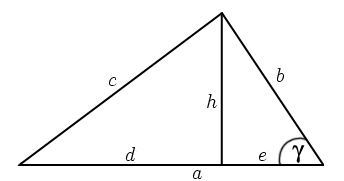
\includegraphics[width=6cm]{./idiotenseite/images/cosinussatz.png}}
\end{tabular}
\begin{center}
	\begin{multicols}{2}
		$\sin \beta = \frac ba =\frac{\text{Gegenkathete}}{\text{Hypotenuse}}$\\
		$\cos \beta = \frac ca =\frac{\text{Ankathete}}{\text{Hypotenuse}}$\\
		$\tan \beta = \frac cb =\frac{\text{Gegenkathete}}{\text{Ankathete}}$\\
		$\cot \beta = \frac cb =\frac{\text{Ankathete}}{\text{Gegenkathete}}$\\
	\end{multicols}
\end{center}

	
\subsection{Funktionswerte für Winkelargumente}
	\begin{multicols}{4}	
	\begin{tabular}[c]{|p{0.5cm}|p{0.4cm}||p{0.5cm}|p{0.5cm}|p{0.5cm}|}
	    	\hline
			deg & rad & sin & cos & tan\\
			\hline
			0\symbol{23} & 0 & 0 & 1 & 0\\
			\hline
			30\symbol{23} & $\frac{\pi}{6}$ & $\frac{1}{2}$ & $\frac{\sqrt{3}}{2}$ &
			$\frac{\sqrt{3}}{3}$\\
			\hline
			45\symbol{23} & $\frac{\pi}{4}$ & $\frac{\sqrt{2}}{2}$ & $\frac{\sqrt{2}}{2}$
			& 1\\
			\hline
			60\symbol{23} & $\frac{\pi}{3}$ & $\frac{\sqrt{3}}{2}$ & $\frac{1}{2}$ &
			$\sqrt{3}$\\
			\hline			
	\end{tabular} \\
	
	\begin{tabular}[c]{|p{0.7cm}|p{0.7cm}||p{0.7cm}|p{0.7cm}|}
	    	\hline
			deg & rad & sin & cos\\
			\hline
			90\symbol{23} & $\frac{\pi}{2}$ & 1 & 0\\
			\hline	
			120\symbol{23} & $\frac{2\pi}{3}$ & $\frac{\sqrt{3}}{2}$ & $-\frac{1}{2}$ \\
			\hline
			135\symbol{23} & $\frac{3\pi}{4}$ & $\frac{\sqrt{2}}{2}$ & $-\frac{\sqrt{2}}{2}$\\
			\hline
			150\symbol{23} & $\frac{5\pi}{6}$ & $\frac{1}{2}$ & $-\frac{\sqrt{3}}{2}$\\
			\hline
	\end{tabular} \\
	
	\begin{tabular}[c]{|p{0.7cm}|p{0.7cm}||p{0.7cm}|p{0.7cm}|}
	  	\hline
		deg & rad & sin & cos\\
		\hline
		180\symbol{23} & $\pi$ & 0 & -1\\
		\hline	
		210\symbol{23} & $\frac{7\pi}{6}$ & $-\frac{1}{2}$ & $-\frac{\sqrt{3}}{2}$\\
		\hline
		225\symbol{23} & $\frac{5\pi}{4}$ & $-\frac{\sqrt{2}}{2}$ & $-\frac{\sqrt{2}}{2}$\\
		\hline
		240\symbol{23} & $\frac{4\pi}{3}$ & $-\frac{\sqrt{3}}{2}$ & $-\frac{1}{2}$\\
		\hline
	\end{tabular} \\
	
	\begin{tabular}[c]{|p{0.7cm}|p{0.7cm}||p{0.7cm}|p{0.7cm}|}
    	\hline
		deg & rad & sin & cos\\
		\hline
		270\symbol{23} & $\frac{3\pi}{2}$ & -1 & 0\\
		\hline	
		300\symbol{23} & $\frac{5\pi}{3}$ & $-\frac{\sqrt{3}}{2}$ & $\frac{1}{2}$\\
		\hline
		315\symbol{23} & $\frac{7\pi}{4}$ & $-\frac{\sqrt{2}}{2}$ & $\frac{\sqrt{2}}{2}$\\
		\hline
		330\symbol{23} & $\frac{11\pi}{6}$ & $-\frac{1}{2}$ & $\frac{\sqrt{3}}{2}$\\
		\hline
	\end{tabular}					
\end{multicols}

\begin{minipage}{13cm}
	\subsection{Periodizität}
	$\cos(a+k\cdot2\pi)=\cos(a) \qquad \sin(a+k\cdot2\pi)=\sin(a) \qquad
	(k \in \mathbb{Z})$
	\subsection{Quadrantenbeziehungen}
	\begin{tabbing}
    	xxxxxxxxxxxxxxxxxxxxxxxxxxxxxxxxxx \= \kill
	  	$\sin(-a)=-\sin(a)$ \> $\cos(-a)=\cos(a)$\\
		$\sin(\pi - a)=\sin(a)$ \> $\cos(\pi - a)=-\cos(a)$\\
		$\sin(\pi + a)=-\sin(a)$ \> $\cos(\pi +a)=-\cos(a)$\\
		$\sin\left(\frac{\pi}{2}-a \right)=\sin\left(\frac{\pi}{2}+a \right)=\cos(a)$ \>
		$\cos\left(\frac{\pi}{2}-a \right)=-\cos\left(\frac{\pi}{2}+a \right)=\sin(a)$  
    \end{tabbing}
\end{minipage}
\begin{minipage}{5cm}
	

\subsection{Ableitungen}

\begin{tikzpicture}
	[	inner sep = 2mm,
		sin/.style={rectangle,minimum width=1.2cm,minimum height=1cm,rounded corners=5pt,draw=black,top color=green!20!black!50},
		abl/.style={rectangle}
	]
	\node at (1.2,0) (sin1) [sin] {$\sin$};
	\node at (0,-1.2) (cos2) [sin] {$-\cos$};
	\node at (1.2,-2.4) (sin2) [sin] {$-\sin$};
	\node at (2.4,-1.2) (cos1) [sin] {$\cos$};
	
	\draw[thick,black,->] (sin1.east) .. controls +(right:0.6cm) and +(up:0.6cm) ..  (cos1.north)
	node [pos=0.5,above](abl) {$\frac{d}{dx}$};
	\draw[thick,black,->] (cos1.south) .. controls +(down:0.6cm) and +(right:0.6cm) .. (sin2.east)
	node [pos=0.5,below](abl) {$\frac{d}{dx}$};
	\draw[thick,black,->] (sin2.west) .. controls +(left:0.6cm) and +(down:0.6cm) .. (cos2.south)
	node [pos=0.5,below](abl) {$\frac{d}{dx}$};
	\draw[thick,black,->] (cos2.north) .. controls +(up:0.6cm) and +(left:0.6cm) .. (sin1.west)
	node [pos=0.5,above](abl) {$\frac{d}{dx}$};
\end{tikzpicture}
\end{minipage}
\begin{multicols}{2}
	\subsection{Additionstheoreme}
	$\sin(a \pm b)=\sin(a) \cdot \cos(b) \pm \cos(a) \cdot \sin(b)$\\
	$\cos(a \pm b)=\cos(a) \cdot \cos(b) \mp \sin(a) \cdot \sin(b)$\\	
	$\tan(a \pm b)=\dfrac{\tan(a) \pm \tan(b)}{1 \mp \tan(a) \cdot \tan(b)}$
	\columnbreak
	
	\subsection{Doppel- und Halbwinkel}	
	$\sin(2a)=2\sin(a)\cos(a)$\\
	$\cos(2a)=\cos^2(a)-\sin^2(a)=2\cos^2(a)-1=1-2\sin^2(a)$\\
	$\cos^2 \left(\frac{a}{2}\right)=\frac{1+\cos(a)}{2} \qquad
	\sin^2 \left(\dfrac{a}{2}\right)=\frac{1-\cos(a)}{2}$
\end{multicols}
\begin{multicols}{2}
	\subsection{Produkte}
		$\sin(a)\sin(b)=\frac{1}{2}(\cos(a-b)-\cos(a+b))$\\
		$\cos(a)\cos(b)=\frac{1}{2}(\cos(a-b)+\cos(a+b))$\\
		$\sin(a)\cos(b)=\frac{1}{2}(\sin(a-b)+\sin(a+b))$\\
	\subsection{Euler-Formeln} 

	$\sin(x) = \frac{1}{2j} \left(e^{jx} - e^{-jx}\right) \qquad
	\cos(x) = \frac{1}{2} \left(e^{jx} + e^{-jx}\right)$ \\
	$e^{x+jy} = e^x \cdot e^{jy} = e^x \cdot \left(\cos(y) + j\sin(y)\right)$ \\
	$e^{j\pi} = e^{-j\pi} = -1$ \\
	\columnbreak
	
	\subsection{Summe und Differenz}
		$\sin(a)+\sin(b)=2 \cdot \sin \left(\frac{a+b}{2}\right) \cdot
		\cos\left(\frac{a-b}{2}\right)$\\
		$\sin(a)-\sin(b)=2 \cdot \sin \left(\frac{a-b}{2}\right) \cdot
		\cos\left(\frac{a+b}{2}\right)$\\
		$\cos(a)+\cos(b)=2 \cdot \cos \left(\frac{a+b}{2}\right) \cdot
		\cos\left(\frac{a-b}{2}\right)$\\
		$\cos(a)-\cos(b)=-2 \cdot \sin \left(\frac{a+b}{2}\right) \cdot
		\sin\left(\frac{a-b}{2}\right)$\\
		$\tan(a) \pm \tan(b)=\dfrac{\sin(a \pm b)}{\cos(a)\cos(b)}$\\
\end{multicols}

\subsection{Quellenumwandlung}
\begin{tabular}{cccp{6cm}}
Lineare Stromquelle		& $\Longleftrightarrow$ & Lineare Spannungsquelle & Formeln \\
\raisebox{-.8\totalheight}{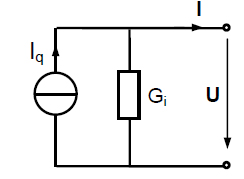
\includegraphics[width=2.8cm]{idiotenseite/images/ersatz_strom.jpg}}&
&
\raisebox{-.8\totalheight}{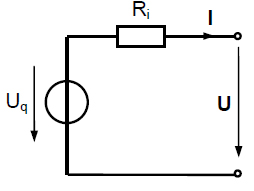
\includegraphics[width=2.8cm]{idiotenseite/images/ersatz_spannung.jpg}}
&
$I_q = \frac{U_q}{R_i} = U_q \cdot G_{i Spannungsquelle}$ \newline
$U_q = \frac{I_q}{G_i} = I_q \cdot R_{i Stromquelle}$ \newline
Der Wiederstand/Leitwert bleibt gleich \newline \\
\end{tabular}
\subsection{Superposition}
\textbf{Vorgehen:}
\begin{multicols}{2}
\begin{enumerate}
  \item Alle Quellen bis auf eine entfernen
  \item Restliche Quellen ersetzen: Stromquelle $\rightarrow$ Unterbruch,
  Spannungsquelle $\rightarrow$ Kurzschluss
  \item Teilströme mit der verbleibenden Quelle berechnen
  \item Für alle anderen Quellen das vorgehen wiederholen
  \item Alle Teilströme/-spannungen zusammenzählen
\end{enumerate}
\end{multicols}
\subsection{Einschaltvorgänge}
\subsubsection{Kondensator}
\input{idiotenseite/elektrotechnik/subsections/einschalt_kondensator}
\subsubsection{Spule}
\input{idiotenseite/elektrotechnik/subsections/einschalt_spule}


\subsection{ohmsche Leistung}
\begin{multicols}{3}
	$P=U \cdot I = I^2 \cdot R = \frac{U^2}{R}$ \\
	$P= I^2 \cdot \omega L = \frac{U^2}{\omega L}$\\
	$P= I^2 \cdot \omega C = \frac{U^2}{\omega C}$
\end{multicols}
\subsection{Strom- Spannungsquellen-Verschiebung}
\input{idiotenseite/tikz/elektrotechnik/UQuellenverschiebung1.tex}
\input{idiotenseite/tikz/elektrotechnik/UQuellenverschiebung2.tex}
\input{idiotenseite/tikz/elektrotechnik/IQuellenverschiebung1.tex}
\input{idiotenseite/tikz/elektrotechnik/IQuellenverschiebung2.tex}      
\subsection{Allgemein zeitabhängige Grössen}
	\begin{tabular}{|ll|ll|}
    \hline
	\multicolumn{2}{|l}{Arithmetischer Mittelwert, Gleichwert, Linearer MW} 
	    	& \multicolumn{2}{l|}{$X_0 = \overline{X} = X_m = \frac {1} {T} \int\limits_{t_0}^{t_0+T}
	    	x(t)dt$} \\
	\hline
	Quadratischer MW, Leistung 
		& $X^2 = \frac {1} {T} \int\limits_{t_0}^{t_0+T} x^2(t)dt$ 
		& MW $n$. Ordnung
		& $X^n = \frac {1} {T} \int\limits_{t_0}^{t_0+T} x^n(t)dt$ \\
	\hline
	Effektivwert (RMS) 
		& $X = \sqrt{X^2} = \sqrt{\frac{1}{T} \int\limits ^{t_0+T}_{t_0}{x^2(t)dt}}$
		& Gleichrichtwert 
		& $X_{|m|} = \bar{|X|} = \frac{1}{T} \int\limits_{t_0}^{t_0+T}{|x(t)| dt}$ \\
	\hline
\end{tabular}
\begin{sidewaystable}
\subsection{Eigenschaften unterschiedlicher Schwingungsformen}
\begin{center}
\begin{tabular}{|l|c|c|c|c|c|c|c|c|}
\hline
	Schwingungsform & Funktion & Gleichrichtwert & Formfaktor &
	Effektivwert & Scheitelfaktor & \textbf{$X_0$} & \textbf{$X^2$} & \textbf{var(X)} \\
\hline
	Formel &
	&
	$\overline{\left|x\right|} = \frac1T\int_{0}^{T}\left| x(t)\right|dt$&
	$\frac{X}{\overline{\left|x\right|}}$&
	$X = \sqrt{X^2} = \sqrt{\frac{1}{T} \int\limits ^{t_0+T}_{t_0}{x^2(t)dt}}$&
	$k_{s}=\frac{X_{\mathrm{max}}}{X_{\mathrm{eff}}}$&
	&
	&
	\\
\hline
	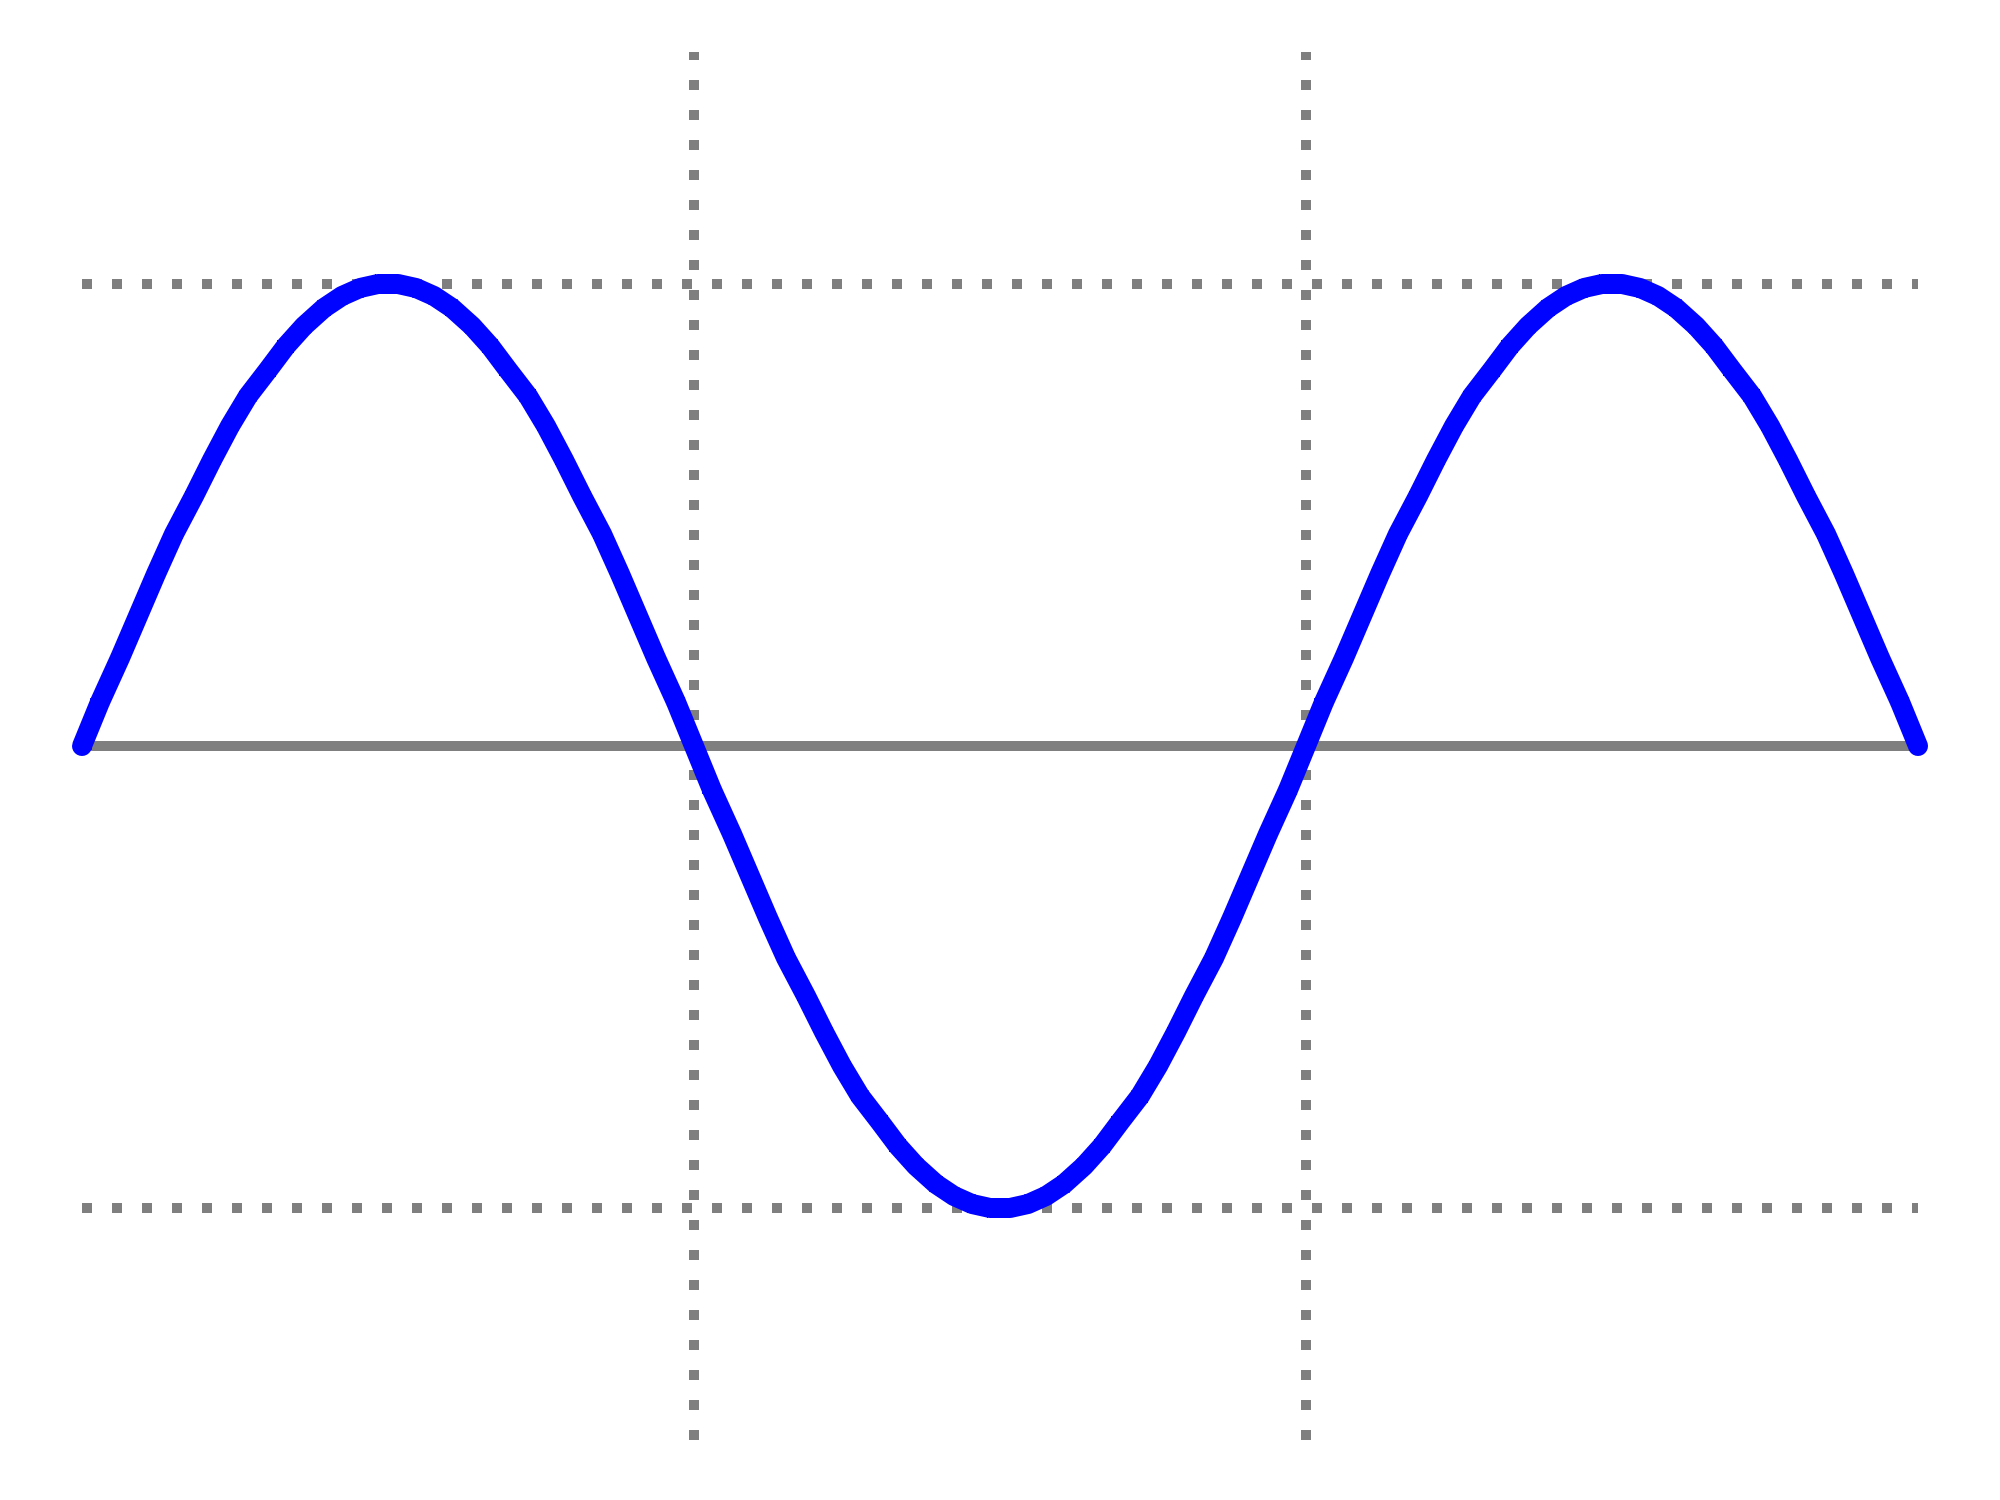
\includegraphics[width=2cm]{idiotenseite/images/table_sine_wave.png} &
	$A\cdot\sin(t)$ &
	$\frac{2}{\pi} \approx 0.637$ &
	$\frac{\pi}{2\sqrt{2}} \approx 1.11$ &
	$\frac{1}{\sqrt{2}}\approx 0.707$ &
	$\sqrt{2}\approx 1.414$ &
	$0$ &
	$\frac{A^2}{2}$ &
	$\frac{A^2}{2}$ \\
\hline	
	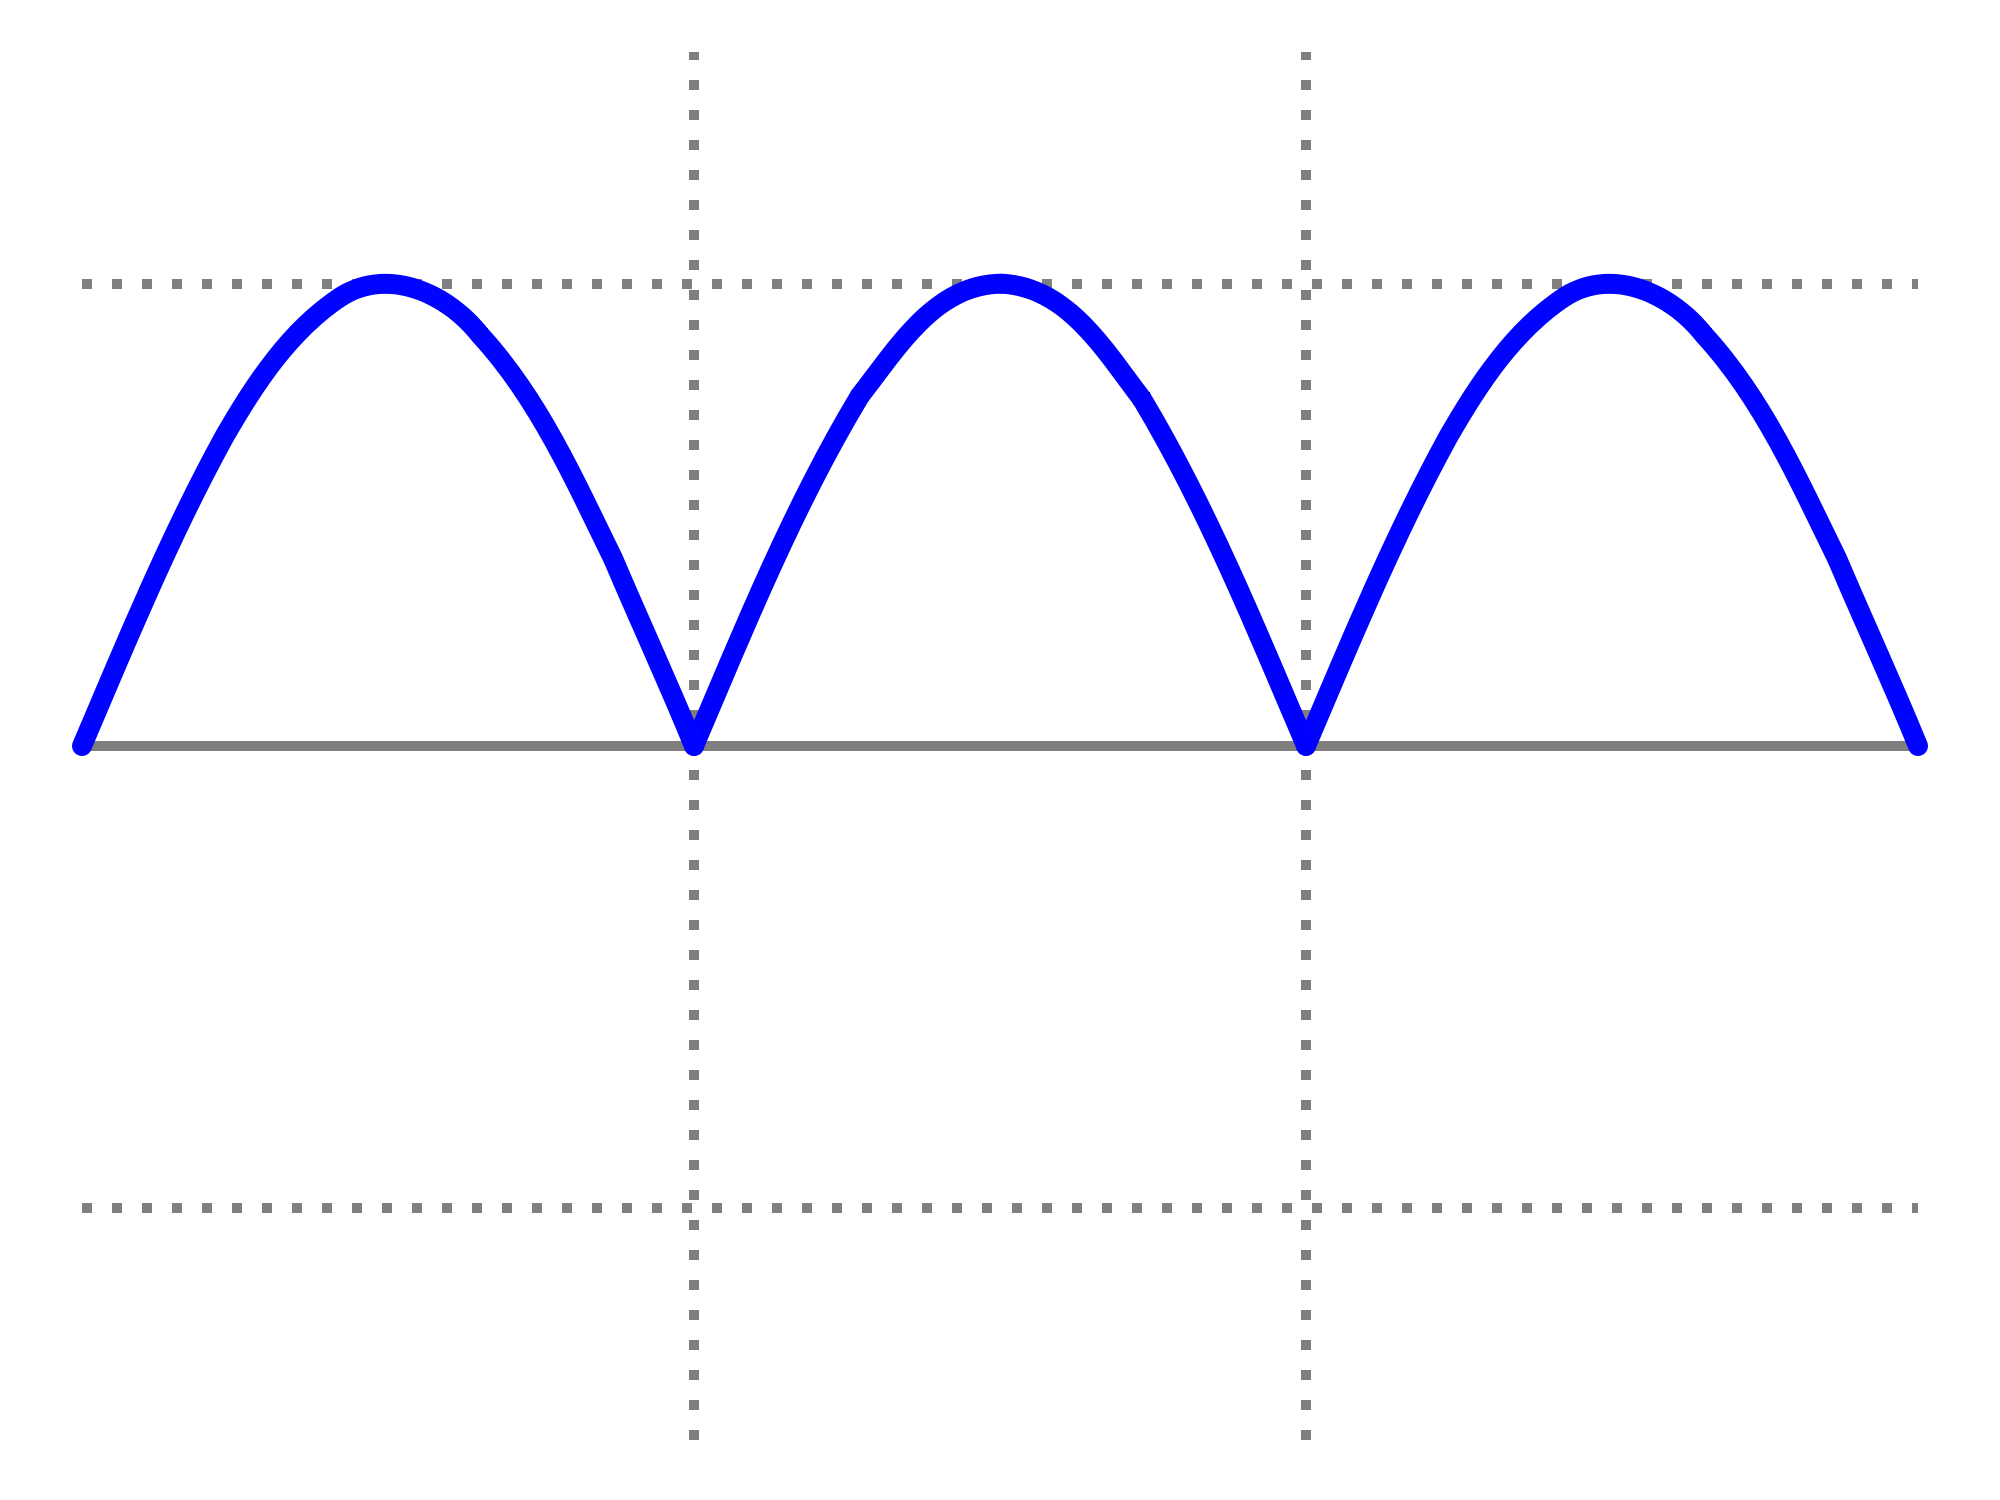
\includegraphics[width=2cm]{idiotenseite/images/table_full-wave_rectified_sine.png} &
	$A\cdot|\sin(t)|$ &
	$\frac{2}{\pi} \approx 0.637$ &
	$\frac{\pi}{2\sqrt{2}} \approx 1.11$ &
	$\frac{1}{\sqrt{2}} \approx 0.707$ &
	$\sqrt{2} \approx 1.414$  &
	$\frac{2A}{\pi}$ & $\frac{A^2}{2}$ & $\frac{A^2}{2}-\frac{4A^2}{\pi^2}$
	\\
\hline
	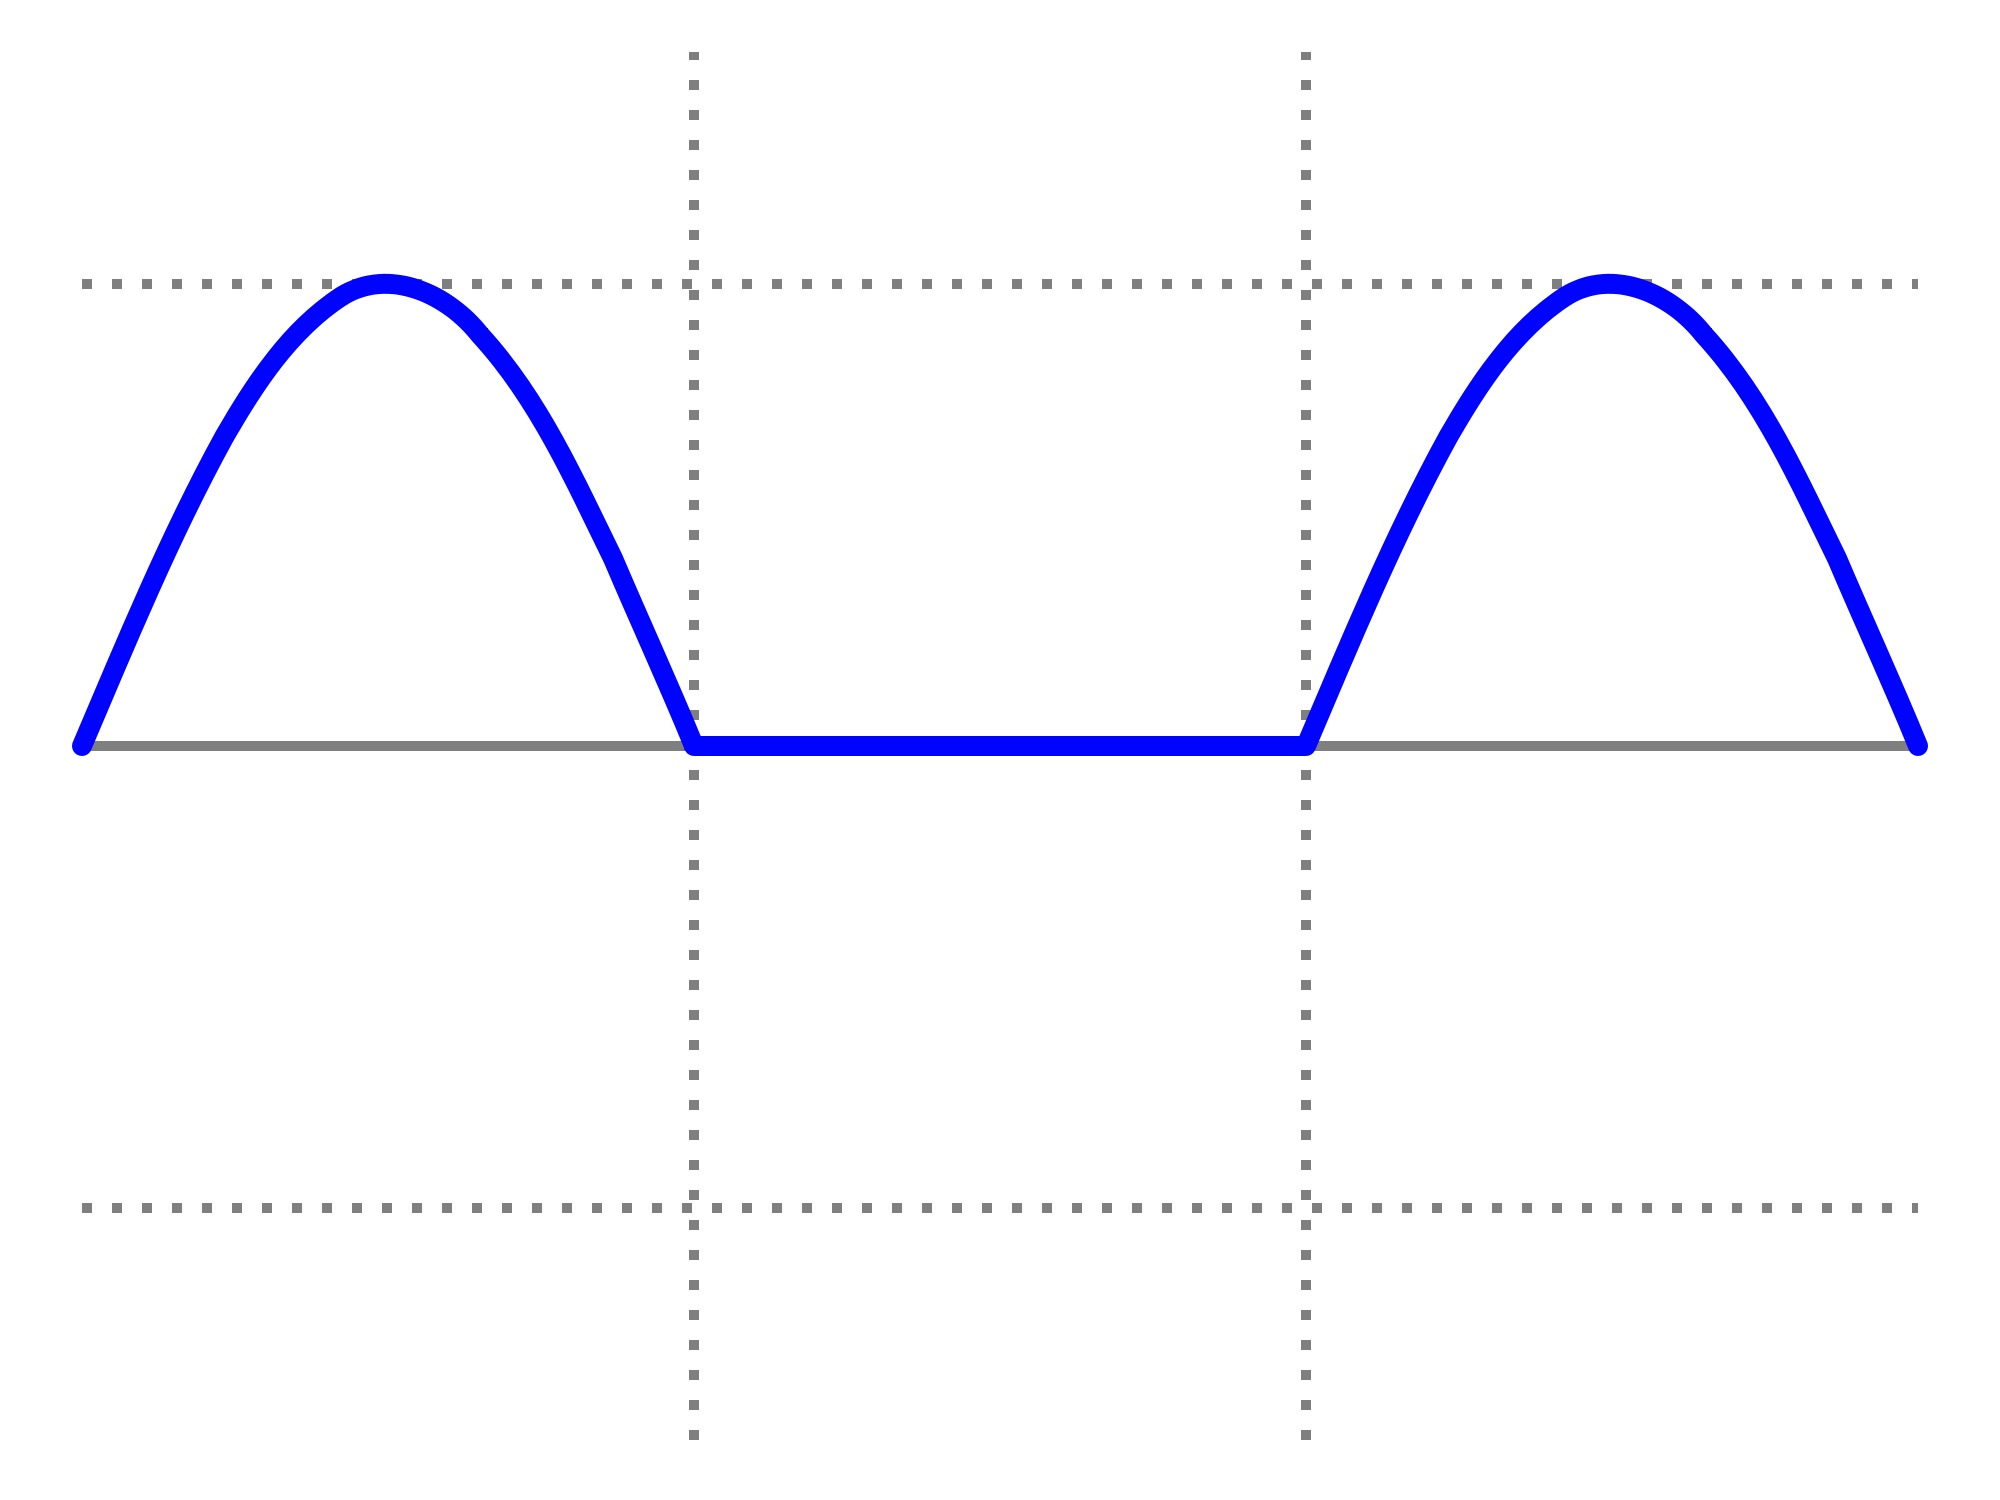
\includegraphics[width=2cm]{idiotenseite/images/table_half-wave_rectified_sine.png} &
	$\begin{cases} A\cdot\sin (t) & 0<t<\pi  \\ 0 & \text{True}\end{cases}$ &
	$\frac{1}{\pi}\approx 0.318$ &
	$\frac{\pi}{2}\approx 1.571$ &
	$\frac{1}{2} = 0.5$	&
	2  &
	$\frac{A}{\pi}$ &
	$\frac{A^2}{4}$ & $\frac{A^2}{4}-\frac{A^2}{\pi^2}$
	\\
\hline
	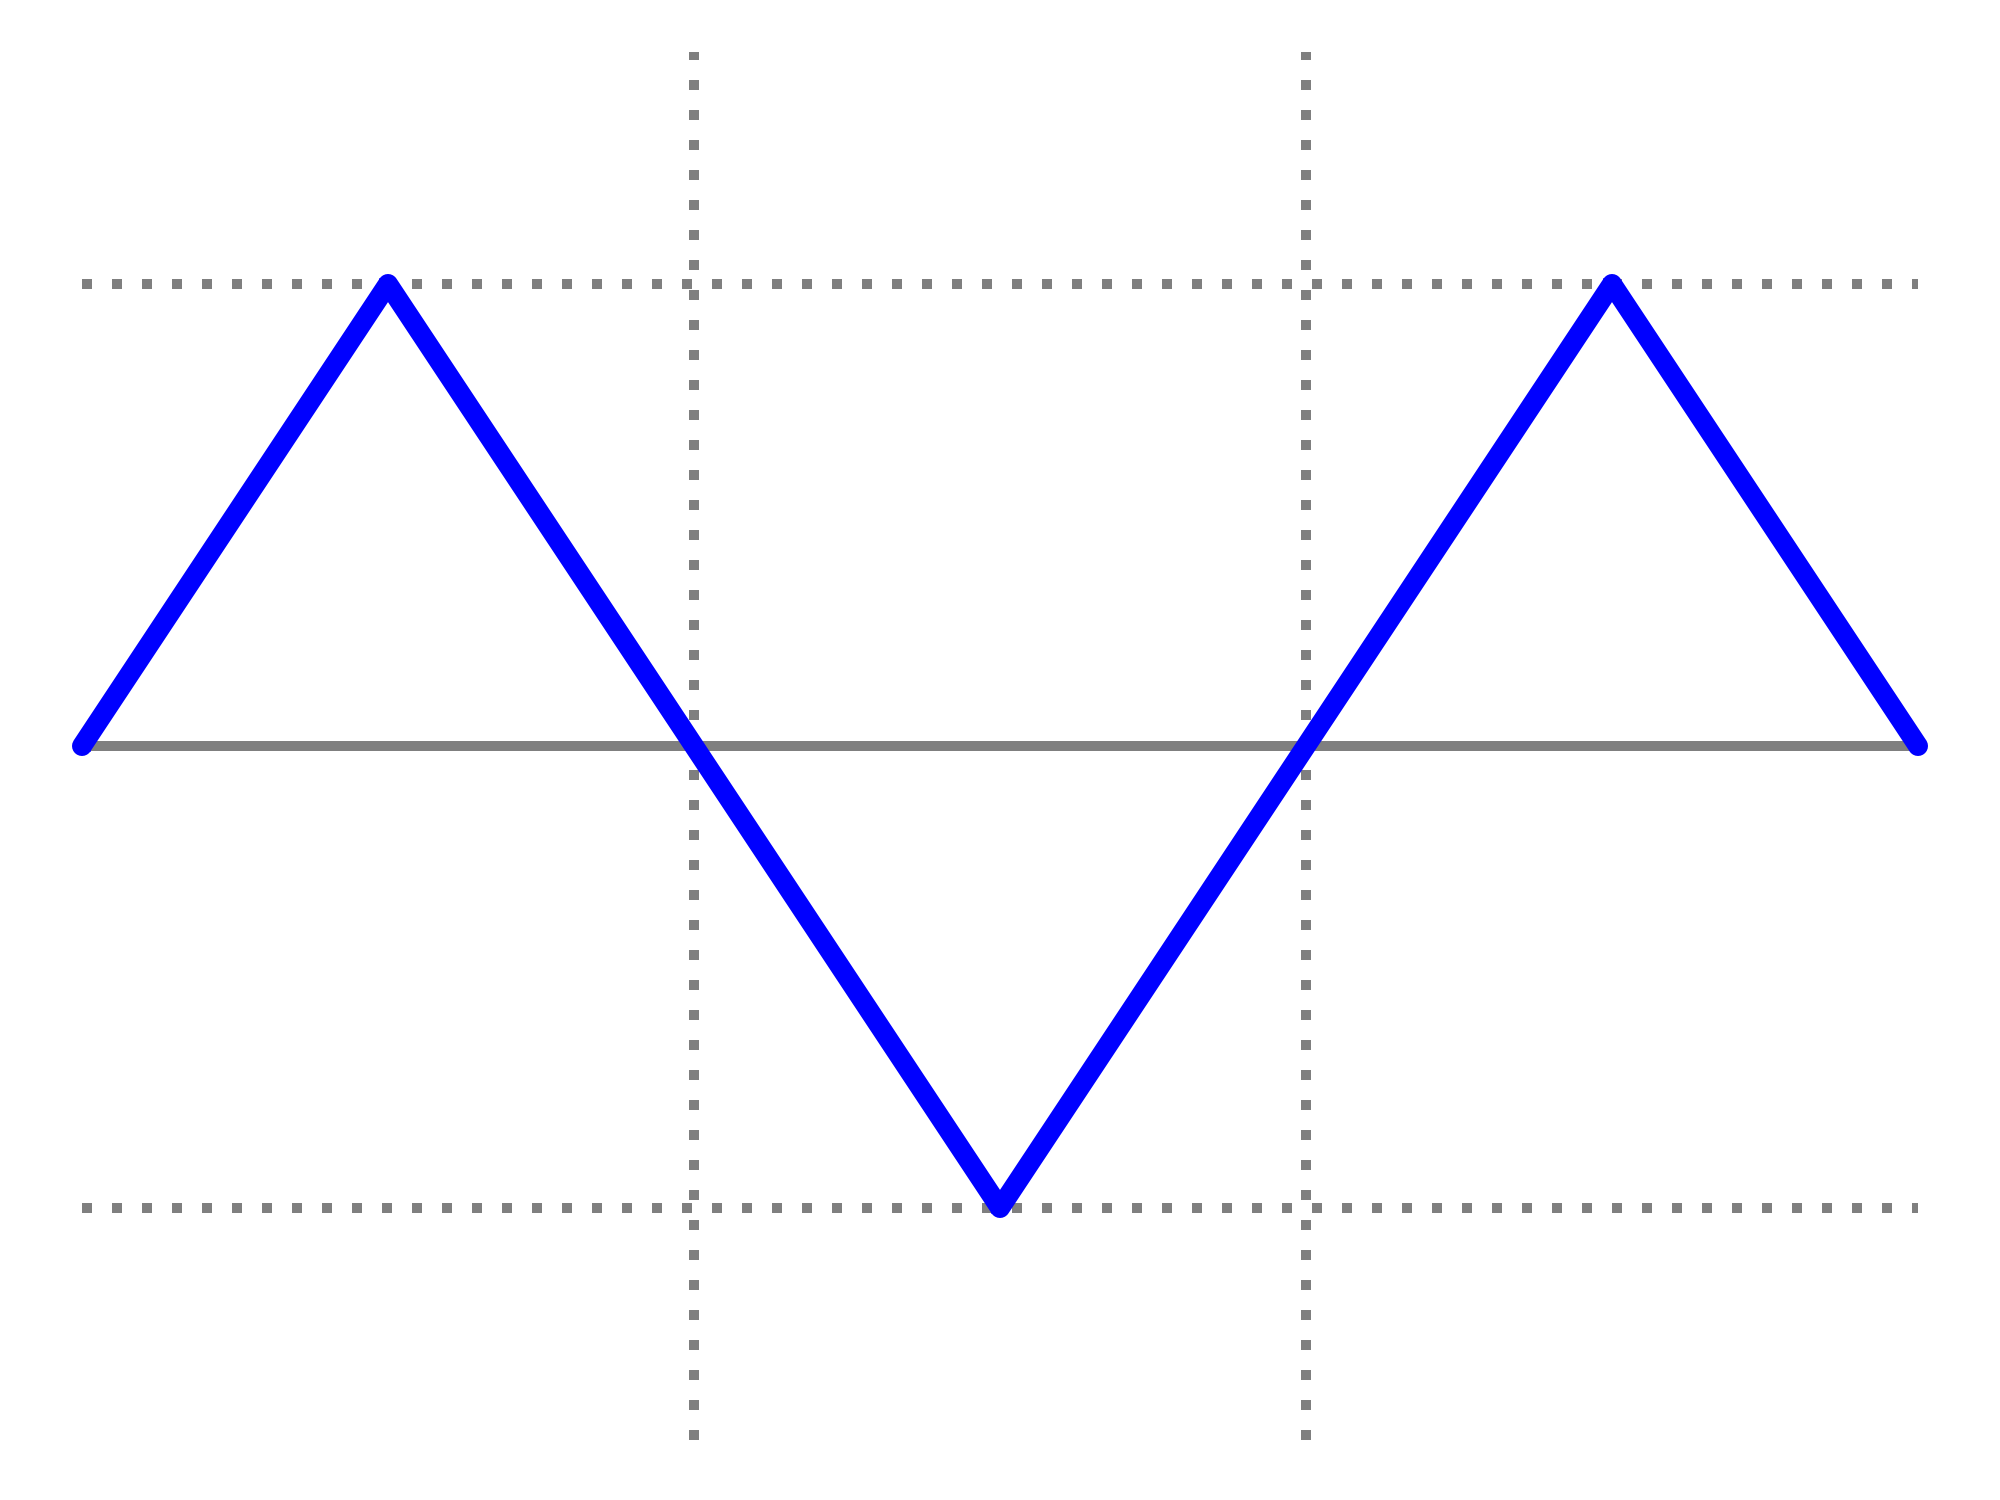
\includegraphics[width=2cm]{idiotenseite/images/table_triangle_wave.png} &
	$A\cdot\Lambda(t)$ &
	$\frac{1}{2}= 0.5$ &
	$\frac{2}{\sqrt{3}}\approx 1.155$ &
	$\frac{1}{\sqrt{3}}
	\approx 0.557$ &
	$\sqrt{3} \approx 1.732$ &
	$0$ &
	$\frac{A^2}{3}$ &
	$\frac{A^2}{3}$ \\
\hline	
	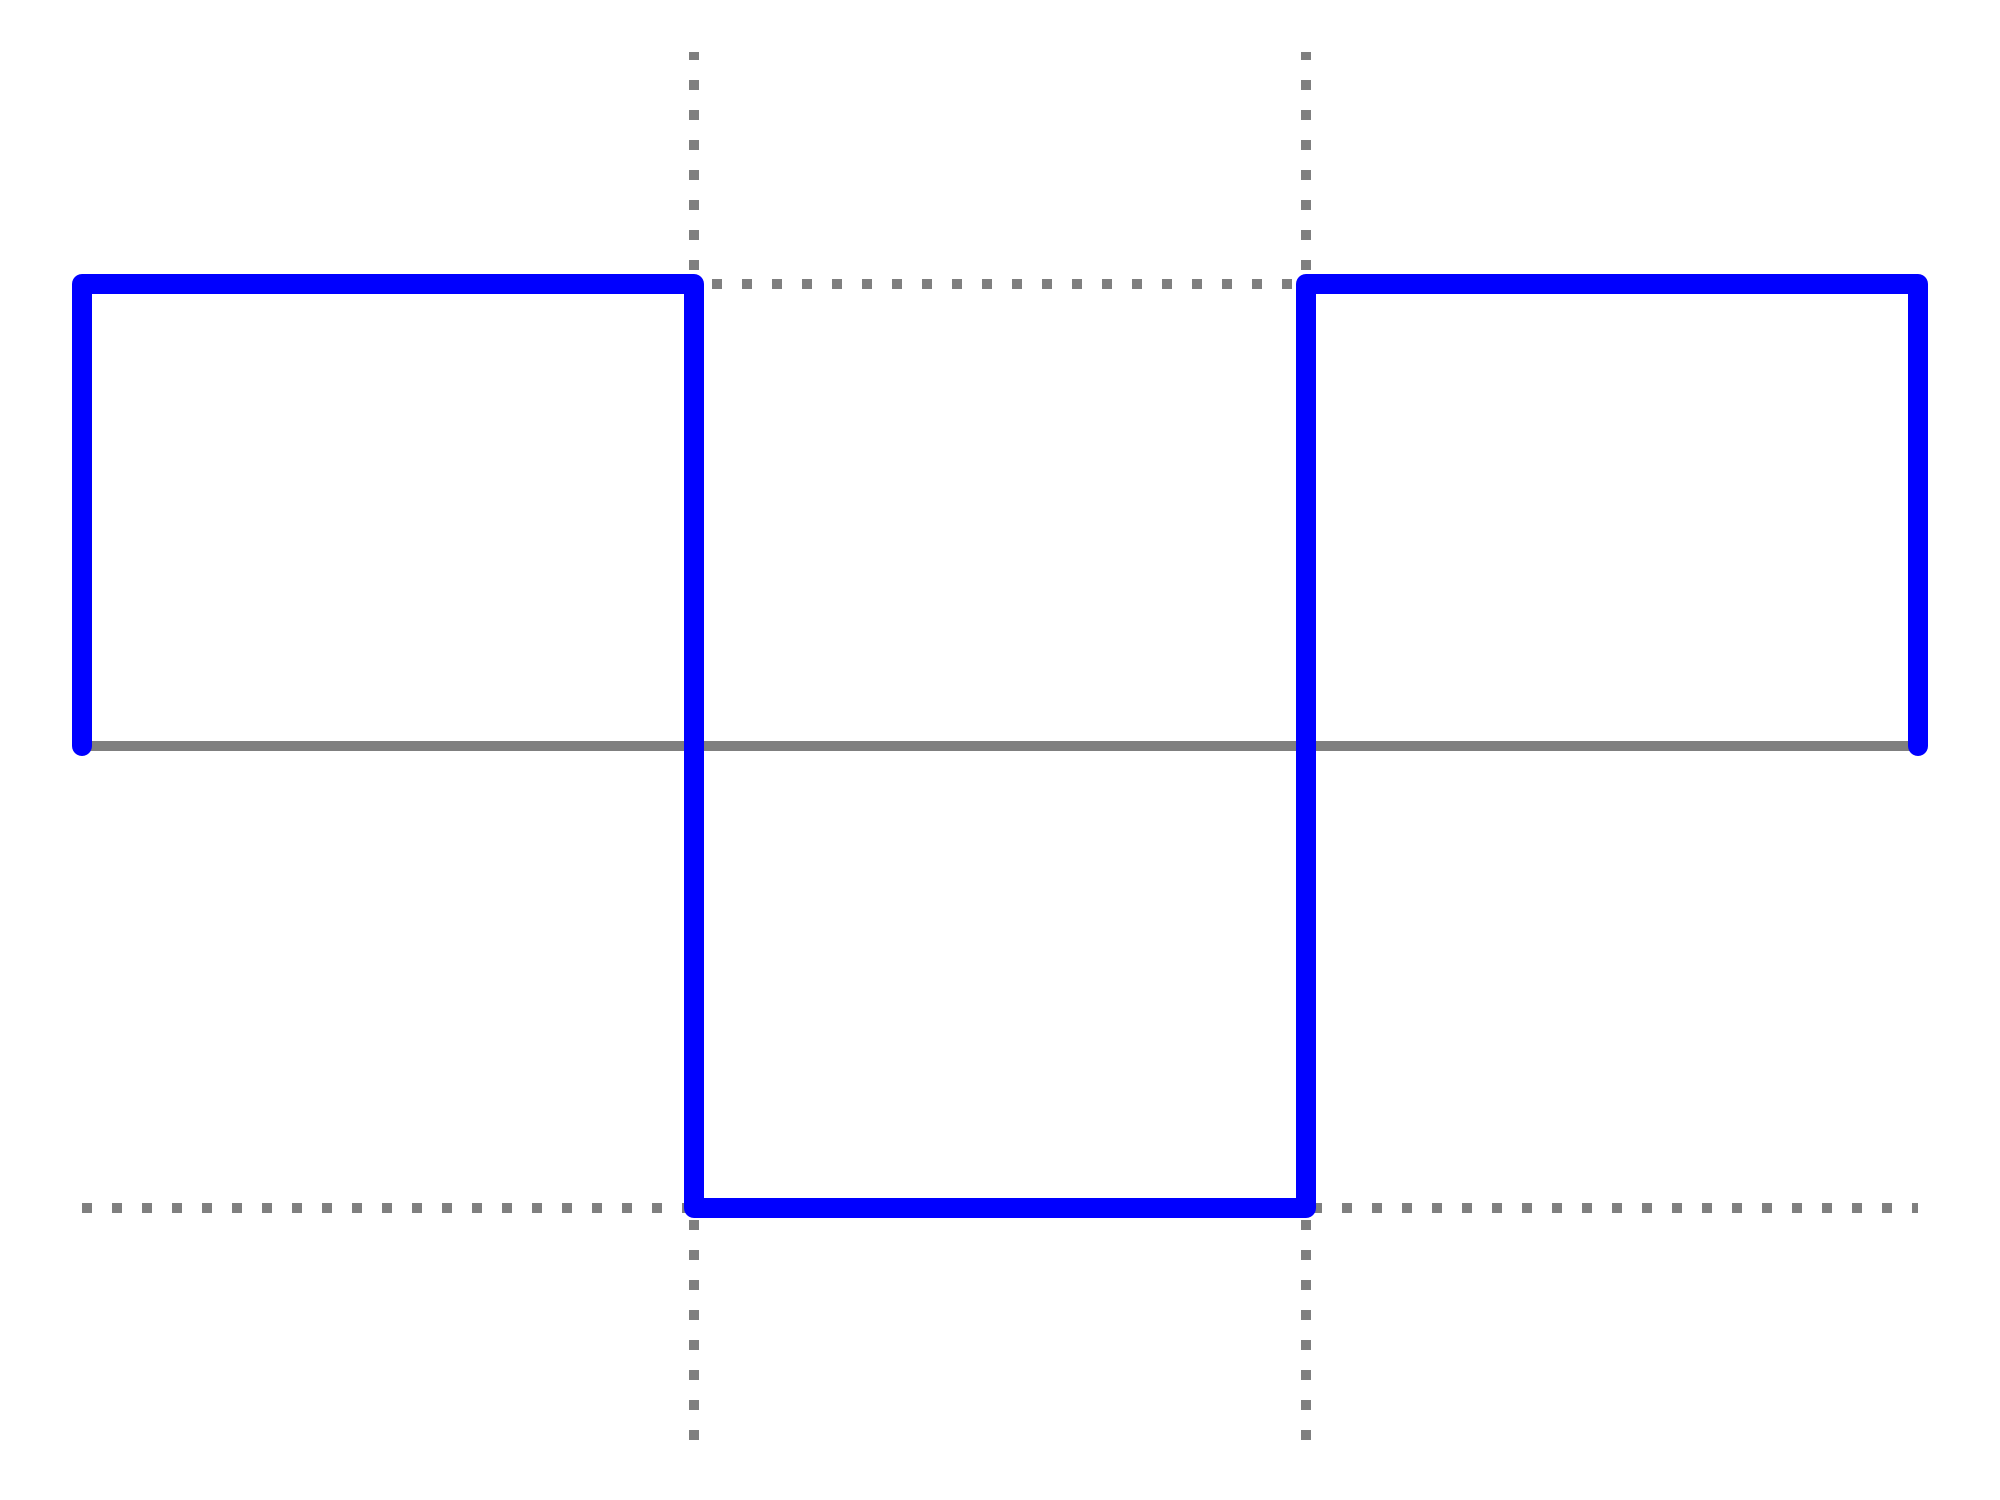
\includegraphics[width=2cm]{idiotenseite/images/table_square_wave.png} &
	$\begin{cases} A & 0<x<t \\ 0 & \text{True}\end{cases}$ &
	$1$ &
	$1$ &
	$1$ &
	$1$ &
	$0$ &
	$A^2$ &
	$A^2$ \\
\hline	
	DC&
	1&
	$1$ &
	$1$ &
	$1$ &
	$1$  &
	-&
	-&
	-\\
\hline	
	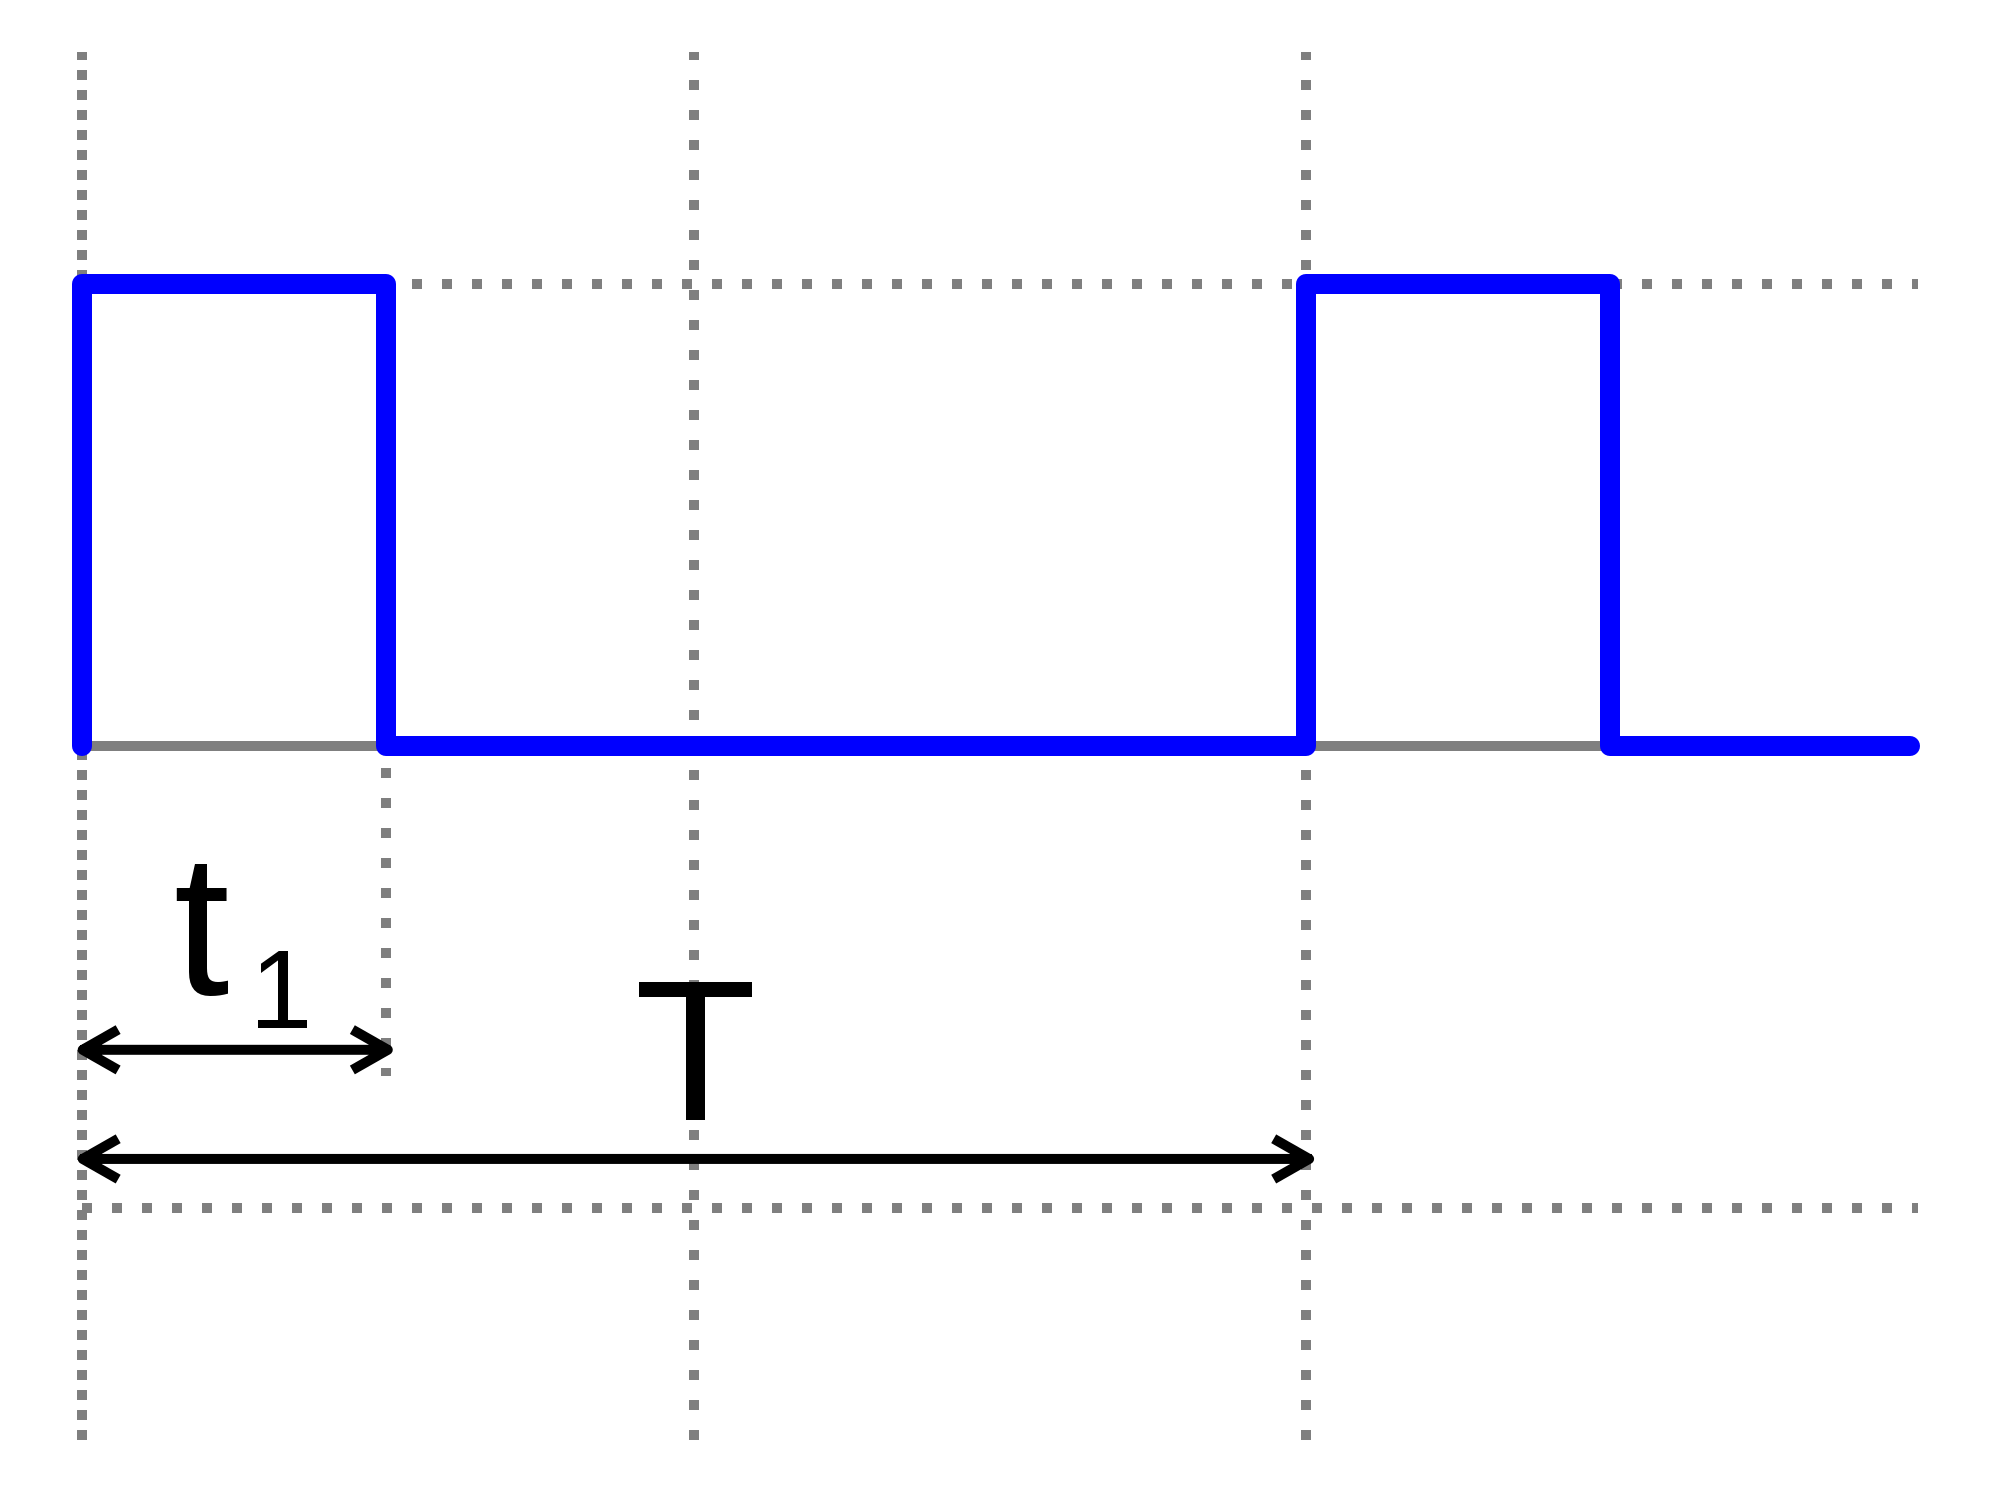
\includegraphics[width=2cm]{idiotenseite/images/table_pulse_wide_wave.png} &
	&
	$\frac{t_1}{T}$ & $\sqrt{\frac{T}{t_1}}$ & $\sqrt{\frac{t_1}{T}}$ & $\sqrt{\frac{T}{t_1}}$ &
	$A\frac{t}{T}$ &
	$A^2\frac{t}{T}$ &
	$\frac{A^2t}{T}-\frac{A^2t^2}{T^2}$\\
\hline
\end{tabular}
\end{center}
\end{sidewaystable}



\subsection{Diverses}
\begin{tabbing}
	xxxxxxxxxxxxxxxxxxxxxxxxxxxx \= xxxxxxxxxxxxxxxxxxxxxxxxxxxxxx \= \kill
 	$f'(z) = \lim \limits_{\Delta z \rightarrow 0} \frac{f(z + \Delta z) -
	f(z)}{\Delta z}$ \> $(a + b)^n = \sum_{k=0}^{n} \binom n k a^{n-k} \cdot b^k$ \>
	$(a \pm b)^3 =a^3 \pm  3 a^{2} b + 3 a b^2 \pm b^3 $\\ \\
	$x_{1,2} = \dfrac{-b \pm \sqrt{b^2 - 4ac}}{2a}$ \> $\binom n k = \dfrac{n!}{k!
	\cdot (n-k)!}$ \> $(a \pm b)^4 =a^4 \pm  4 a^{3} b + 6a^2b^2 \pm 4 a b^3 +
	b^4$\\
\end{tabbing}
\subsection{Reihenentwicklungen}
\begin{tabular}{llll}
\textbf{Geometrische Reihe}
	& $\sum\limits_{n=0}^{\infty} x^n$ 
	& $= \dfrac{1}{1-x}$
	& $|x| < 1$ \\
	
	& $\sum\limits_{k=0}^{\infty} k \, x^k$ & $= x \sum\limits_{k=1}^{\infty} k \,
	x^{k-1} = \dfrac{x}{(1-x)^2} $ 
	& $x \neq 1$ \\
    & $\sum\limits_{k=0}^{n} a_0\cdot q^k$ & $= a_0 \dfrac{1-q^{n+1}}{1-q}$
    & $q \neq 1$\\
\textbf{Binominalreihe} 
	& $\sum\limits_{n=0}^\infty \binom{\alpha}{n} x^n $ &$= (1+x)^\alpha$
	& $x \in (-1,1)$ \\
\textbf{E-Funktion}
	& $\sum\limits_{k = 0}^{\infty} \dfrac{x^k}{k!}$ &$ = e^x$
	& 
\end{tabular}

\subsection{Kurven}
\begin{multicols}{4}
\subsubsection{e-Funktion}
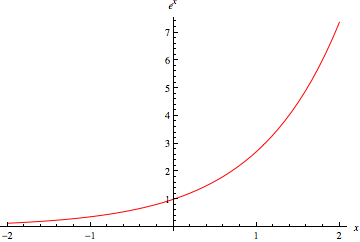
\includegraphics[width=4.5cm]{idiotenseite/images/Exp.png}
\subsubsection{Sinus-Funktion}
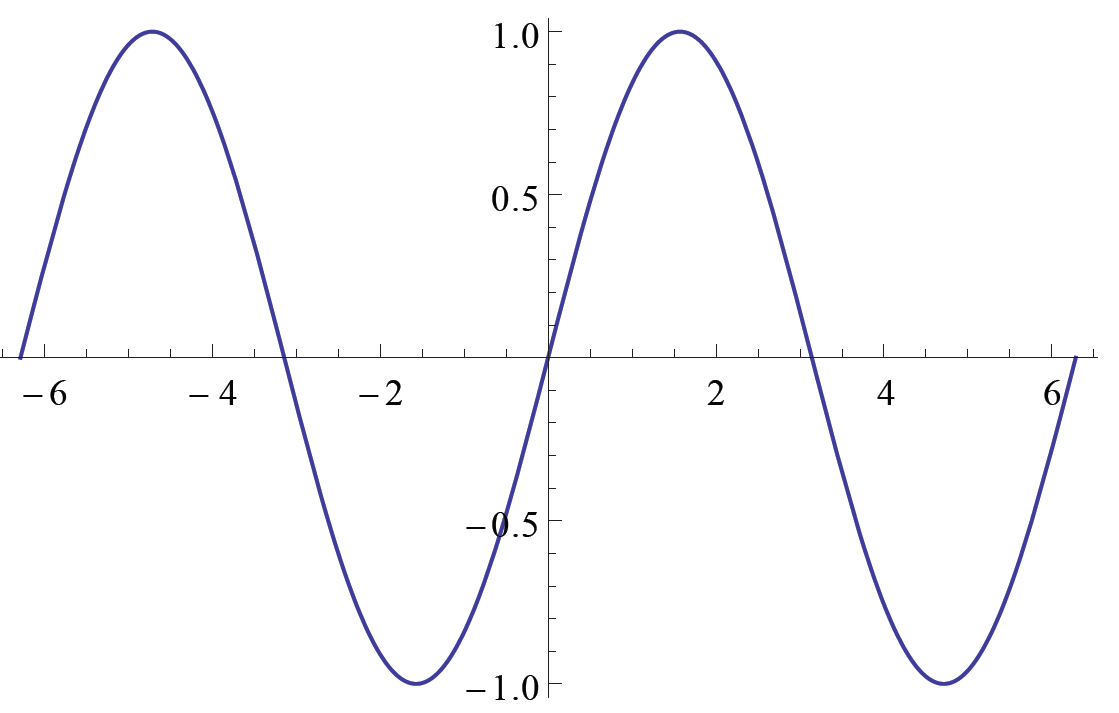
\includegraphics[width=4.5cm]{idiotenseite/images/sin.png}
\subsubsection{Cosinus-Funktion}
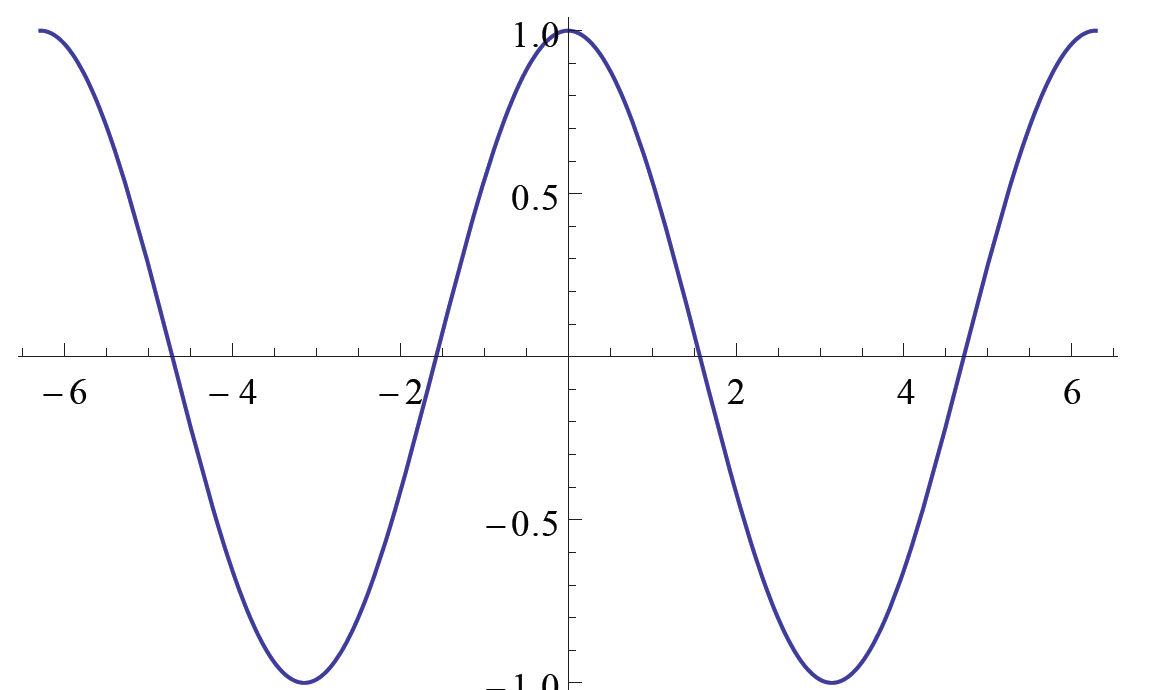
\includegraphics[width=4.5cm]{idiotenseite/images/cos.png}
\subsubsection{Tangens-Funktion}
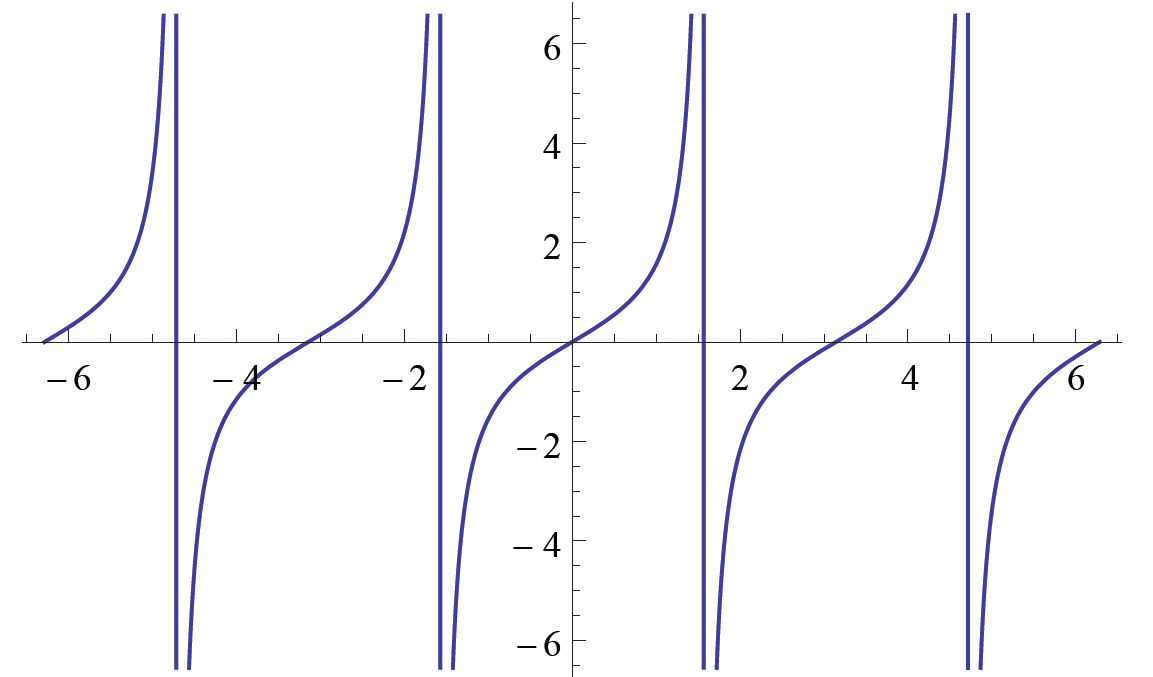
\includegraphics[width=4.5cm]{idiotenseite/images/tan.png}
\end{multicols}
%\subsection{Idiotenformel}
Wenn ihr wissen wollt was die Formel besagt dann kauft euch doch nächstes mal
die Pro Version der Formelsammlung. Arme Schmarotzer und asoziale Personen
dürfen gerne lange darüber Rätseln was das hier soll. Aber wer zu doof ist eine
Formelsammlung ehrlich zu erwerben hat sowieso keine Chance. Haha.\\
$\frac{1}{F_{Siedlungsfl\ddot ache}}\cdot\int\limits_{\vec{x} \in
Siedlungsfl\ddot ache} \frac{1}{\int\limits_{\vec{y}\in Siedlungsfl\ddot ache\ und \left|\vec{x}-\vec{y} \right|<BH}\vec{dy}} \int\limits_{\vec{y}\in Siedlungsfl\ddot ache\ und \left|\vec{x}-\vec{y} \right|<BH} \sqrt{\frac{2\cdot\left|\vec{x}-\vec{y}\right|}{1m}+1}-1\vec{dy}\vec{dx}\frac{DSE}{m^2}$

\subsection{SI-Vorsätze}

\begin{multicols}{2}
\begin{tabular}{|l|l|l|l|}
\hline
\textbf{Symbol}	& \textbf{Name} & \textbf{Wert} & \textbf{Binär} \\
\hline
da	& Deka 	& $10^1$ & \\
\hline
h	& Hekto & $10^2$ & \\ 
\hline
k	& Kilo	& $10^3$ & $2^{10} = 1024$ \\
\hline
M	& Mega	& $10^6$ & $2^{20}$\\
\hline
G	& Giga  & $10^9$ & $2^{30}$\\
\hline
T	& Tera	& $10^{12}$ & $2^{40}$ \\
\hline
P	& Peta	& $10^{15}$ & $2^{50}$\\
\hline
\end{tabular}

\columnbreak

\begin{tabular}{|l|l|l|}
\hline
\textbf{Symbol}	& \textbf{Name} & \textbf{Wert} \\
\hline
d	& Dezi	& $10^{-1}$ \\
\hline
c	& Centi	& $10^{-2}$ \\ 
\hline
m	& Milli	& $10^{-3}$ \\
\hline
y, $\mu$ & Mikro & $10^{-6}$ \\
\hline
n	& Nano	& $10^{-9}$ \\
\hline
p	& Piko	& $10^{-12}$ \\
\hline
f	& Femto & $10^{-15}$ \\
\hline
\end{tabular}
\end{multicols}
\subsection{GrichischesAlphabet}
\begin{multicols}{2}
	\subsubsection{klein}
	\begin{tabular}{ |l|l|l|l|l|l|l|l|}
		\hline
		$\alpha$&Alpha&$\theta$&Theta&o&o&$\tau$&Tau\\
		\hline
		$\beta$&Beta&$\vartheta$&Theta&$\pi$&Pi&$\upsilon$&Ypsilon\\
		\hline
		$\gamma$&Gamma&$\gamma$&Gamma&$\varpi$&Pi&$\phi$&Phi\\
		\hline
		$\delta$&Delta&$\kappa$&Kappa&$\rho$&Roh&$\varphi$&Phi\\
		\hline
		$\epsilon$&Epsilon&$\lambda$&Lambda&$\varrho$&Roh&$\chi$&Chi\\
		\hline
		$\varepsilon$&Epsilon&$\mu$&Mu&$\sigma$&Sigma&$\psi$&Psi\\
		\hline
		$\zeta$&Zeta&$\nu$&Nu&$\varsigma$&Sigma&$\omega$&Omega\\
		\hline
		$\eta$&Eta&$\xi$&Xi&&&&\\
		\hline
	\end{tabular}
	\columnbreak
	
	\subsubsection{gross}
	\begin{tabular}{|l|l|l|l|l|l|l|l|}
		\hline
		$\Gamma$&Gamma&$\Lambda$&Lambda&$\Sigma$&Sigma&$\Psi$&Psi\\
		\hline
		$\Delta$&Delta&$\Xi$&Xi&$\Upsilon$&Ypsilon&$\Omega$&Omega\\
		\hline
		$\Theta$&Theta&$\Pi$&Pi&$\Phi$&Phi&&\\
		\hline
	\end{tabular}
\end{multicols}
\begin{sidewaystable}
\subsection{Einige unbestimmte Integrale\buchSeite{1074}}
\label{unbestimmte_integrale}
\begin{tabular}{|p{12cm}|p{12cm}|}
  \hline
  
    $ \int dx=x+C $ &
     $ \int{x^\alpha}dx=\frac{x^{\alpha+1}}{\alpha+1}+C,\ x \epsilon \mathbb
    R ^+,\ \alpha \epsilon \mathbb R \backslash \{ -1 \} $ \\\hline
     $ \int{\frac{1}{x}}dx=\ln \left| x \right| + C,\ x\neq0 $ &
     $ \int{e^x}dx=e^x+C $ \\\hline
     $ \int{a^x}dx=\frac{a^x}{\ln{a}}+C,\ a \epsilon \mathbb 
    R^+\backslash\{1\} $ &
     $ \int{ \sin{x}} dx = -\cos{x} + C $ \\\hline
     $ \int{\cos{x}} dx = \sin{x} + C $ &
     $ \int{\frac{dx}{\sin^2x}}=-\cot{x}+C,\ x\neq k\pi\ \mathrm{mit}\ k
    \epsilon \mathbb Z $ \\\hline
     $ \int{\frac{dx}{\cos^2x}}=\tan{x}+C,\ x\neq\frac{\pi}{2}+k\pi\
    \mathrm{mit} k \epsilon \mathbb Z $ & 
    
    %10. :
     $ \int{\sinh{x}}dx = \cosh{x}+C $ \\ \hline
     $ \int{\cosh{x}}dx = \sinh{x}+C $ &
     $ \int{\frac{dx}{\sinh^2x}}=-\coth{x}+C,\ x\neq0 $ \\\hline
     $ \int{\frac{dx}{\cosh^2x}}=\tanh{x}+C $ &
     $ \int{\frac{dx}{ax+b}} = \frac{1}{a}\ln \left|ax + b\right| + C,\
    a\neq 0,x\neq-\frac{b}{a} $ \\\hline
     $ \int{\frac{dx}{a^2x^2+b^2}}=\frac{1}{ab}\arctan{\frac{a}{b}x}+C,\
    a\neq0,\ b\neq0 $ &
     $
    \int{\frac{dx}{a^2x^2-b^2}}=\frac{1}{2ab}\ln{\left|\frac{ax-b}{ax+b}\right|}+C,\
    a\neq0,\ b\neq0,\ x\neq\frac{b}{a},\ x\neq-\frac{b}{a} $ \\\hline
     $
    \int{\sqrt{a^2x^2+b^2}}dx=\frac{x}{2}\sqrt{a^2x^2+b^2}+\frac{b^2}{2a}\ln{(ax+\sqrt{a^2x^2+b^2})}+C,\
    a\neq0,\ b\neq0 $ &
     $
    \int{\sqrt{a^2x^2-b^2}}dx=\frac{x}{2}\sqrt{a^2x^2-b^2}-\frac{b^2}{2a}\ln\left|ax+\sqrt{a^2x^2-b^2}\right|+C,\
    a\neq0,\ b\neq0,a^2x^2\geqq b^2$ \\\hline
     $
    \int\sqrt{b^2-a^2x^2}dx=\frac{x}{2}\sqrt{b^2-a^2x^2}+\frac{b^2}{2a}\arcsin\frac{a}{b}x+C,\
    a\neq0,\ b\neq0,\ a^2x^2\leqq b^2 $ &
    %20.:
     $
    \int\frac{dx}{\sqrt{a^2x^2-b^2}}=\frac{1}{a}\ln(ax+\sqrt{a^2x^2+b^2})+C,\
    a\neq0,\ b\neq0 $ \\\hline
     $
    \int\frac{dx}{\sqrt{a^2x^2-b^2}}=\frac{1}{a}\ln\left|ax+\sqrt{a^2x^2-b^2}\right|+C,\
    a\neq0,\ b\neq0,\ a^2x^2>b^2 $ &
     $ \int\frac{dx}{\sqrt{b^2-a^2x^2}}=\frac{1}{a}\arcsin\frac{a}{b}x+C,\
    a\neq0,\ b\neq0,\ a^2x^2<b^2 $ \\\hline
     Die Integrale $\int\frac{dx}{X}, \int\sqrt{X}dx,
    \int\frac{dx}{\sqrt{X}}$ mit $X=ax^2+2bx+c,\ a\neq0 $ werden durch 
    die Umformung $X=a(x+\frac{b}{a})^2+(c-\frac{b^2}{a}) $ und die
    Substitution $ t=x+\frac{b}{a} $ in die oberen 4 Zeilen
    transformiert. & $ \int\frac{xdx}{X}=\frac{1}{2a}\ln\left|X\right|-\frac{b}{a}\int\frac{dx}{X},\
    a\neq0,\ X=ax^2+2bx+c $ \\\hline
     $ \int\sin^2axdx=\frac{x}{2}-\frac{1}{4a}\cdot\sin2ax+C,\ a\neq0 $ &
     $ \int\cos^2axdx=\frac{x}{2}+\frac{1}{4a}\cdot\sin2ax+C,\ a\neq0 $ \\\hline
     $ \int\sin^naxdx=-\frac{sin^{n-1}ax\cdot\cos
    ax}{na}+\frac{n-1}{n}\int\sin^{n-2}axdx,\ n \epsilon \mathbb N,\ a\neq0 $ &
     $ \int\cos^naxdx=\frac{\cos^{n-1}ax\cdot\sin
    ax}{na}+\frac{n-1}{n}\int\cos^{n-2}axdx,\ n\epsilon \mathbb N,\ a\neq0 $
    \\\hline
     $ \int\frac{dx}{\sin ax} =
    \frac{1}{a}\ln\left|\tan\frac{ax}{2}\right|+C,\ a\neq0,\ x\neq
    k\frac{\pi}{a}\ \mathrm{mit}\ k\epsilon\mathbb Z$ &
    %30.:
     $ \int\frac{dx}{\cos
    ax}=\frac{1}{a}\ln\left|\tan(\frac{ax}{2}+\frac{\pi}{4})\right|+C,\ a\neq0,\
    x\neq\frac{\pi}{2a}+k\frac{\pi}{a}\ \mathrm{mit}\ k\epsilon\mathbb Z $
    \\\hline
     $\int\tan axdx=-\frac{1}{a}\ln\left|\cos ax\right|+C,\ a\neq0,\
    x\neq\frac{\pi}{2a}+k\frac{\pi}{a} \mathrm{mit}\ k\epsilon\mathbb Z$ &
     $\int\cot axdx=\frac{1}{a}\ln\left|\sin ax\right|+C,\ a\neq0,\ x\neq
    k\frac{\pi}{a} \mathrm{mit} k\epsilon\mathbb Z $ \\ \hline
     $ \int x^n\sin axdx=-\frac{x^n}{a}\cos ax+\frac{n}{a}\int x^{n-1}\cos
    axdx,\ n\epsilon\mathbb N,\ a\neq0 $ &
    $ \int x^n\cos axdx=\frac{x^n}{a}\sin ax-\frac{n}{a}\int x^{n-1}\sin
    axdx,\ n\epsilon\mathbb N,\ a\neq0 $ \\ \hline
     $ \int x^ne^{ax}dx=\frac{1}{a}x^ne^{ax}-\frac{n}{a}\int
    x^{n-1}e^{ax}dx,\ n\epsilon\mathbb N,\ a\neq0 $ &
     $ \int e^{ax}\sin bxdx=\frac{e^{ax}}{a^2+b^2}(a\sin bx-b\cos bx)+C,\
    a\neq0,\ b\neq0 $  \\ \hline
     $ \int e^{ax}\cos bxdx=\frac{e^{ax}}{a^2+b^2}(a\cos bx + b\sin bx)+C,\
    a\neq0,\ b\neq0 $ &
     $ \int\ln x dx = x(\ln x-1)+C,\ x\epsilon\mathbb R^+ $ \\ \hline
     $ \int x^\alpha \cdot \ln xdx =
    \frac{x^{\alpha+1}}{(\alpha+1)^2}\lbrack(\alpha+1)\ln x-1\rbrack + C,\
    x\epsilon\mathbb R^+,\ \alpha\epsilon\mathbb R\backslash\{-1\} $ & \\ \hline
    %FF1 Seite 496
    
\end{tabular}
\end{sidewaystable}

%\begin{sidewaystable}
\subsection{Ableitungen elementarer Funktionen\formelbuch{436}}
\label{unbestimmte_integrale}
\renewcommand{\arraystretchOriginal}{2.5}
\begin{tabular}{|l|l||l|l|}
  \hline
  \textbf{Funktion} & \textbf{Ableitung} & \textbf{Funktion} &
  \textbf{Ableitung}\\\hline
  $C$ (Konstante) & 0 & $\sec x$ & $\dfrac{\sin x}{\cos^2 x}$ \\
  $x$ & 1 & $\sec^{-1} x$ & $\dfrac{-\cos x}{\sin^2 x}$\\
  $x^n$ ($n\in\mathbb{R}$) & $nx^{n-1}$ & $\arcsin x \quad (|x| < 1)$ &
  $\dfrac{1}{\sqrt{1-x^2}}$\\
  $\dfrac{1}{x}$ & $-\dfrac{1}{x^2}$ & $\arccos x \quad (|x| < 1)$ &
  $-\dfrac{1}{\sqrt{1-x^2}}$\\
  $\dfrac{1}{x^n}$ & $-\dfrac{n}{x^{n+1}}$ & $\arctan x$ & $\dfrac{1}{1+x^2}$\\
  $\sqrt{x}$ & $\dfrac{1}{2\sqrt{x}}$ & arccot $x$ & $-\dfrac{1}{1+x^2}$\\
  $\sqrt[n]{x}\quad (n\in\mathbb{R}, n \neq 0, x > 0)$ &
  $\dfrac{1}{n\sqrt[n]{x^{n-1}}}$ & arcsec $x$ & $\dfrac{1}{x\sqrt{x^2-1}}$\\
  $\mathrm{e}^x$ & $\mathrm{e}^x$ & arcossec $x$ & $-\dfrac{1}{x\sqrt{x^2-1}}$\\
  $\mathrm{e}^{bx}\quad (b\in\mathbb{R})$ & $b\mathrm{e}^{bx}$ & $\sinh x$ &
  $\cosh x$\\
  $a^x\quad (a > 0)$ & $a^x\ln a$ & $\cosh x$ & $\sinh x$\\
  $a^{bx}\quad (b\in\mathbb{R}, a > 0)$ & $ba^{bx}\ln a$ & $\tanh x$ &
  $\dfrac{1}{\cosh^2 x}$\\
  $\ln x$ & $\dfrac{1}{x}$ & $\coth x \quad(x \neq 0)$ & $-\dfrac{1}{\sinh^2 x}$\\
  $\log_a{x} \quad (a > 0, a \neq 1, x > 0)$ &
  $\dfrac{1}{x}\log_a{\mathrm{e}}=\dfrac{1}{x\ln a}$ & Arsinh $x$ &
  $\dfrac{1}{\sqrt{1+x^2}}$\\
  $\lg x \quad (x > 0)$ & $\dfrac{1}{x}\lg \mathrm{e}\approx \dfrac{0.4343}{x}$
  & Arcosh $x \quad (x > 1)$ & $\dfrac{1}{\sqrt{x^2-1}}$\\
  $\sin x$ & $\cos x$ & Artanh $x \quad (|x| < 1)$ & $\dfrac{1}{1-x^2}$\\
  $\cos x$ & $-\sin x$ & Arcoth $x \quad (|x| > 1)$ & $-\dfrac{1}{x^2-1}$\\
  $\tan x \quad (x\neq(2k+1)\dfrac{\pi}{2}, k\in\mathbb{Z})$ & $\dfrac{1}{\cos^2
  x}=\sec^2 x$ & $[f(x)]^n \quad (n\in\mathbb{R})$ & $n[f(x)]^{n-1}f'(x)$\\
  $\cot x \quad (x\neq k\pi, k\in\mathbb{Z})$ & $\dfrac{-1}{\sin^2 x}=-cosec^2x$ & $\ln f(x) \quad (f(x)> 0)$ & $\dfrac{f'(x)}{f(x)}$\\
  \hline
\end{tabular}
\renewcommand{\arraystretchOriginal}{1.5}
%\end{sidewaystable}



\end{document}